\documentclass[a4paper,14pt]{extarticle} %,twoside


%Добавление ангстрема
\newcommand{\angstrom}{\mbox{\normalfont\AA}}



%%% Проверка используемого TeX-движка %%%
\usepackage{iftex}
\newif\ifxetexorluatex   % определяем новый условный оператор (http://tex.stackexchange.com/a/47579/79756)
\ifXeTeX
    \xetexorluatextrue
\else
    \ifLuaTeX
        \xetexorluatextrue
    \else
        \xetexorluatexfalse
    \fi
\fi

%%% Поля и разметка страницы %%%
\usepackage{pdflscape}                              % Для включения альбомных страниц
\usepackage{geometry}                               % Для последующего задания полей

%%% Математические пакеты %%%
\usepackage{amsthm,amsfonts,amsmath,amssymb,amscd}  % Математические дополнения от AMS
\usepackage{mathtools}                              % Добавляет окружение multlined

%%%% Установки для размера шрифта 14 pt %%%%
%% Формирование переменных и констант для сравнения (один раз для всех подключаемых файлов)%%
%% должно располагаться до вызова пакета fontspec или polyglossia, потому что они сбивают его работу
\newlength{\curtextsize}
\newlength{\bigtextsize}
\setlength{\bigtextsize}{13.9pt}

\makeatletter
%\show\f@size                                       % неплохо для отслеживания, но вызывает стопорение процесса, если документ компилируется без команды  -interaction=nonstopmode 
\setlength{\curtextsize}{\f@size pt}
\makeatother

%%% Кодировки и шрифты %%%
\ifxetexorluatex
    \usepackage{polyglossia}                        % Поддержка многоязычности (fontspec подгружается автоматически)
\else
    \RequirePDFTeX                                  % tests for PDFTEX use and throws an error if a different engine is being used
   %%% Решение проблемы копирования текста в буфер кракозябрами
%    \input glyphtounicode.tex
%    \input glyphtounicode-cmr.tex %from pdfx package
%    \pdfgentounicode=1
    \usepackage{cmap}                               % Улучшенный поиск русских слов в полученном pdf-файле
    \defaulthyphenchar=127                          % Если стоит до fontenc, то переносы не впишутся в выделяемый текст при копировании его в буфер обмена
    \usepackage[T2A]{fontenc}                       % Поддержка русских букв
    \usepackage[utf8]{inputenc}                     % Кодировка utf8
    \usepackage[english, russian]{babel}            % Языки: русский, английский
    \IfFileExists{pscyr.sty}{\usepackage{pscyr}}{}  % Красивые русские шрифты
\fi

%%% Оформление абзацев %%%
\usepackage{indentfirst}                            % Красная строка

%%% Цвета %%%
\usepackage[dvipsnames,usenames]{color}
\usepackage{colortbl}
%\usepackage[dvipsnames, table, hyperref, cmyk]{xcolor} % Вероятно, более новый вариант, вместо предыдущих двух строк. Конвертация всех цветов в cmyk заложена как удовлетворение возможного требования типографий. Возможно конвертирование и в rgb.

%%% Таблицы %%%
\usepackage{longtable}                              % Длинные таблицы
\usepackage{multirow,makecell,array}                % Улучшенное форматирование таблиц
\usepackage{booktabs}                               % Возможность оформления таблиц в классическом книжном стиле (при правильном использовании не противоречит ГОСТ)

%%% Общее форматирование
\usepackage{soulutf8}                               % Поддержка переносоустойчивых подчёркиваний и зачёркиваний
\usepackage{icomma}                                 % Запятая в десятичных дробях


%%% Гиперссылки %%%
\usepackage{hyperref}

%%% Изображения %%%
\usepackage{graphicx}                               % Подключаем пакет работы с графикой

%%% Списки %%%
\usepackage{enumitem}

%%% Подписи %%%
\usepackage{caption}                                % Для управления подписями (рисунков и таблиц) % Может управлять номерами рисунков и таблиц с caption %Иногда может управлять заголовками в списках рисунков и таблиц
\usepackage{subcaption}                             % Работа с подрисунками и подобным

%%% Интервалы %%%
\usepackage[onehalfspacing]{setspace}               % Опция запуска пакета правит не только интервалы в обычном тексте, но и формульные

%%% Счётчики %%%
\usepackage[figure,table]{totalcount}               % Счётчик рисунков и таблиц
\usepackage{totcount}                               % Пакет создания счётчиков на основе последнего номера подсчитываемого элемента (может требовать дважды компилировать документ)
\usepackage{totpages}                               % Счётчик страниц, совместимый с hyperref (ссылается на номер последней страницы). Желательно ставить последним пакетом в преамбуле

%%% Продвинутое управление групповыми ссылками (пока только формулами) %%%
\ifxetexorluatex
    \usepackage{cleveref}                           % cleveref корректно считывает язык из настроек polyglossia
\else
    \usepackage[russian]{cleveref}                  % cleveref имеет сложности со считыванием языка из babel. Такое решение русификации вывода выбрано вместо определения в documentclass из опасности что-то лишнее передать во все остальные пакеты, включая библиографию.
\fi
\creflabelformat{equation}{#2#1#3}                  % Формат по умолчанию ставил круглые скобки вокруг каждого номера ссылки, теперь просто номера ссылок без какого-либо дополнительного оформления

                % Пакеты общие для диссертации и автореферата
%%% Опционально %%%
% Следующий пакет может быть полезен, если надо ужать текст, чтобы сам текст не править, но чтобы места он занимал поменьше
%\usepackage{savetrees}

% Этот пакет может быть полезен для печати текста брошюрой
%\usepackage[print]{booklet}         % Пакеты для автореферата
\usepackage{tabularx,tabulary}  %таблицы с автоматически подбирающейся шириной столбцов

% Листинги с исходным кодом программ
\usepackage{fancyvrb}
\usepackage{listings}

% Плавающие окружения. во многом лучше пакета float
\usepackage{floatrow}

% Русская традиция начертания греческих букв
%\usepackage{upgreek} % прямые греческие ради русской традиции        % Пакеты для специфических пользовательских задач 

% Новые переменные, которые могут использоваться во всём проекте
\newcommand{\authorbibtitle}{Публикации автора}
\newcommand{\fullbibtitle}{Список литературы} % (ГОСТ Р 7.0.11-2011, 4)
     % Новые переменные, которые могут использоваться во всём проекте
%%%%%%%%%%%%%%%%%%%%%%%%%%%%%%%%%%%%%%%%%%%%%%%%%%%%%%
%%%% Файл упрощённых настроек шаблона диссертации %%%%
%%%%%%%%%%%%%%%%%%%%%%%%%%%%%%%%%%%%%%%%%%%%%%%%%%%%%%

%%%        Подключение пакетов                 %%%
\usepackage{ifthen}                 % добавляет ifthenelse
%%% Инициализирование переменных, не трогать!  %%%
\newcounter{bibliosel}
\newcounter{tabcap}
\newcounter{tablaba}
\newcounter{tabtita}
%%%%%%%%%%%%%%%%%%%%%%%%%%%%%%%%%%%%%%%%%%%%%%%%%%

%%% Область упрощённого управления оформлением %%%

%% Библиография

%% Внимание! При использовании bibtex8 необходимо удалить все
%% цитирования из  ../common/characteristic.tex 
\setcounter{bibliosel}{1}           % 0 --- встроенная реализация с загрузкой файла через движок bibtex8; 1 --- реализация пакетом biblatex через движок biber

%% Подпись таблиц
\setcounter{tabcap}{0}              % 0 --- по ГОСТ, номер таблицы и название разделены тире, выровнены по левому краю, при необходимости на нескольких строках; 1 --- подпись таблицы не по ГОСТ, на двух и более строках, дальнейшие настройки: 
%Выравнивание первой строки, с подписью и номером
\setcounter{tablaba}{2}             % 0 --- по левому краю; 1 --- по центру; 2 --- по правому краю
%Выравнивание строк с самим названием таблицы
\setcounter{tabtita}{1}             % 0 --- по левому краю; 1 --- по центру; 2 --- по правому краю

%%% Цвета гиперссылок %%%
% Latex color definitions: http://latexcolor.com/
\definecolor{linkcolor}{rgb}{0.9,0,0}
\definecolor{citecolor}{rgb}{0,0.6,0}
\definecolor{urlcolor}{rgb}{0,0,1}
%\definecolor{linkcolor}{rgb}{0,0,0} %black
%\definecolor{citecolor}{rgb}{0,0,0} %black
%\definecolor{urlcolor}{rgb}{0,0,0} %black               % Упрощённые настройки шаблона 

%%% Основные сведения %%%
\newcommand{\thesisAuthor}             % Диссертация, ФИО автора
{%
    \texorpdfstring{% \texorpdfstring takes two arguments and uses the first for (La)TeX and the second for pdf
        {Ярославцев Алексей Алексеевич}% так будет отображаться на титульном листе или в тексте, где будет использоваться переменная
    }{%
        Ярославцев, Алексей Алексеевич% эта запись для свойств pdf-файла. В таком виде, если pdf будет обработан программами для сбора библиографических сведений, будет правильно представлена фамилия.
    }%
}
\newcommand{\thesisUdk}                % Диссертация, УДК
{\todo{xxx.xxx}}
\newcommand{\thesisTitle}              % Диссертация, название
{\texorpdfstring{{\textbf{ВЛИЯНИЕ ЛОКАЛЬНОГО ОКРУЖЕНИЯ МЕДИ НА МАГНИТНЫЕ И ТРАНСПОРТНЫЕ СВОЙСТВА СОЕДИНЕНИЙ ГРУППЫ ТЕТРАЭДРИТА-ТЕННАНТИТА}}}{Название диссертационной работы}}

%ВЛИЯНИЕ ИЗОВАЛЕТНОГО ЗАМЕЩЕНИЯ В СОЕДИНЕНИЯХ Cu\textsubscript{12}V\textsubscript{4}VI\textsubscript{13} (V~=~As,~Sb И VI~=~S,~Se) НА МАГНИТНЫЕ И ТРАНСПОРТНЫЕ СВОЙСТВА

\newcommand{\thesisSpecialtyNumber}    % Диссертация, специальность, номер
{\texorpdfstring{{01.03.08}}{XX.XX.XX}}
\newcommand{\thesisSpecialtyTitle}     % Диссертация, специальность, название
{\texorpdfstring{{Физика конденсированного состояния}}{Название специальности}}
\newcommand{\thesisDegree}             % Диссертация, научная степень
{{кандидата физико-математических наук}}
\newcommand{\thesisCity}               % Диссертация, город защиты
{{Москва}}
\newcommand{\thesisYear}               % Диссертация, год защиты
{{2021}}
\newcommand{\thesisOrganization}       % Диссертация, организация
{{Федеральное государственное бюджетное научное учреждение «Технологический институт сверхтвердых и новых углеродных материалов», (ФГБНУ ТИСНУМ)}}

\newcommand{\thesisInOrganization}       % Диссертация, организация в предложном падеже: Работа выполнена в ...
{{Федеральном государственном бюджетном научном учреждении «Технологический институт сверхтвердых и новых углеродных материалов» (ФГБНУ ТИСНУМ).}}

\newcommand{\supervisorFio}            % Научный руководитель, ФИО
{Буга Сергей Геннадьевич}
\newcommand{\supervisorRegalia}        % Научный руководитель, регалии
{доктор физико-математических наук, доцент}

\newcommand{\opponentOneFio}           % Оппонент 1, ФИО
{\todo{Фамилия Имя Отчество}}
\newcommand{\opponentOneRegalia}       % Оппонент 1, регалии
{\todo{доктор физико-математических наук, профессор}}
\newcommand{\opponentOneJobPlace}      % Оппонент 1, место работы
{\todo{Не очень длинное название для места работы}}
\newcommand{\opponentOneJobPost}       % Оппонент 1, должность
{\todo{старший научный сотрудник}}

\newcommand{\opponentTwoFio}           % Оппонент 2, ФИО
{\todo{Фамилия Имя Отчество}}
\newcommand{\opponentTwoRegalia}       % Оппонент 2, регалии
{\todo{кандидат физико-математических наук}}
\newcommand{\opponentTwoJobPlace}      % Оппонент 2, место работы
{\todo{Основное место работы c длинным длинным длинным длинным названием}}
\newcommand{\opponentTwoJobPost}       % Оппонент 2, должность
{\todo{старший научный сотрудник}}

\newcommand{\leadingOrganizationTitle} % Ведущая организация, дополнительные строки
{\todo{Федеральное государственное бюджетное образовательное учреждение высшего профессионального образования с~длинным длинным длинным длинным названием}}

\newcommand{\defenseDate}              % Защита, дата
{\todo{DD mmmmmmmm YYYY~г.~в~XX часов}}
\newcommand{\defenseCouncilNumber}     % Защита, номер диссертационного совета
{\todo{NN}}
\newcommand{\defenseCouncilTitle}      % Защита, учреждение диссертационного совета
{\todo{Название учреждения}}
\newcommand{\defenseCouncilAddress}    % Защита, адрес учреждение диссертационного совета
{\todo{Адрес}}

\newcommand{\defenseSecretaryFio}      % Секретарь диссертационного совета, ФИО
{\todo{Фамилия Имя Отчество}}
\newcommand{\defenseSecretaryRegalia}  % Секретарь диссертационного совета, регалии
{\todo{д-р~физ.-мат. наук}}            % Для сокращений есть ГОСТы, например: ГОСТ Р 7.0.12-2011 + http://base.garant.ru/179724/#block_30000

\newcommand{\synopsisLibrary}          % Автореферат, название библиотеки
{\todo{Название библиотеки}}
\newcommand{\synopsisDate}             % Автореферат, дата рассылки
{\todo{DD mmmmmmmm YYYY года}}

\newcommand{\keywords}%                 % Ключевые слова для метаданных PDF диссертации и автореферата
{}                     % Основные сведения
%%% Макет страницы %%%
% Выставляем значения полей (ГОСТ 7.0.11-2011, 5.3.7)
\geometry{a4paper,top=2cm,bottom=2cm,left=2.5cm,right=1cm}

%%% Кодировки и шрифты %%%
\ifxetexorluatex
    \setmainlanguage[babelshorthands=true]{russian}  % Язык по-умолчанию русский с поддержкой приятных команд пакета babel
    \setotherlanguage{english}                       % Дополнительный язык = английский (в американской вариации по-умолчанию)
    \ifXeTeX
        \defaultfontfeatures{Ligatures=TeX,Mapping=tex-text}
    \else
        \defaultfontfeatures{Ligatures=TeX}
    \fi
    \setmainfont{Times New Roman}
    \newfontfamily\cyrillicfont{Times New Roman}
    \setsansfont{Arial}
    \newfontfamily\cyrillicfontsf{Arial}
    \setmonofont{Courier New}
    \newfontfamily\cyrillicfonttt{Courier New}
\else
    \IfFileExists{pscyr.sty}{\renewcommand{\rmdefault}{ftm}}{}
\fi

%%% Интервалы %%%
%linespread-реализация ближе к реализации полуторного интервала в ворде.
%setspace реализация заточена под шрифты 10, 11, 12pt, под остальные кегли хуже, но всё же ближе к типографской классике. 
%\linespread{1.3}                    % Полуторный интервал (ГОСТ Р 7.0.11-2011, 5.3.6)

%%% Выравнивание и переносы %%%
\sloppy                             % Избавляемся от переполнений
\clubpenalty=10000                  % Запрещаем разрыв страницы после первой строки абзаца
\widowpenalty=10000                 % Запрещаем разрыв страницы после последней строки абзаца

%%% Подписи %%%
\captionsetup{%
singlelinecheck=off,                % Многострочные подписи, например у таблиц
skip=2pt,                           % Вертикальная отбивка между подписью и содержимым рисунка или таблицы определяется ключом
justification=centering,            % Центрирование подписей, заданных командой \caption
}

%%% Рисунки %%%
\DeclareCaptionLabelSeparator*{emdash}{~--- }             % (ГОСТ 2.105, 4.3.1)
\captionsetup[figure]{labelsep=emdash,font=onehalfspacing,position=bottom}

%%% Таблицы %%%
\ifthenelse{\equal{\thetabcap}{0}}{%
    \newcommand{\tabcapalign}{\raggedright}  % по левому краю страницы или аналога parbox
}

\ifthenelse{\equal{\thetablaba}{0} \AND \equal{\thetabcap}{1}}{%
    \newcommand{\tabcapalign}{\raggedright}  % по левому краю страницы или аналога parbox
}

\ifthenelse{\equal{\thetablaba}{1} \AND \equal{\thetabcap}{1}}{%
    \newcommand{\tabcapalign}{\centering}    % по центру страницы или аналога parbox
}

\ifthenelse{\equal{\thetablaba}{2} \AND \equal{\thetabcap}{1}}{%
    \newcommand{\tabcapalign}{\raggedleft}   % по правому краю страницы или аналога parbox
}

\ifthenelse{\equal{\thetabtita}{0} \AND \equal{\thetabcap}{1}}{%
    \newcommand{\tabtitalign}{\raggedright}  % по левому краю страницы или аналога parbox
}

\ifthenelse{\equal{\thetabtita}{1} \AND \equal{\thetabcap}{1}}{%
    \newcommand{\tabtitalign}{\centering}    % по центру страницы или аналога parbox
}

\ifthenelse{\equal{\thetabtita}{2} \AND \equal{\thetabcap}{1}}{%
    \newcommand{\tabtitalign}{\raggedleft}   % по правому краю страницы или аналога parbox
}

\DeclareCaptionFormat{tablenocaption}{\tabcapalign #1\strut}        % Наименование таблицы отсутствует
\ifthenelse{\equal{\thetabcap}{0}}{%
    \DeclareCaptionFormat{tablecaption}{\tabcapalign #1#2#3}
    \captionsetup[table]{labelsep=emdash}                       % тире как разделитель идентификатора с номером от наименования
}{%
    \DeclareCaptionFormat{tablecaption}{\tabcapalign #1#2\par%  % Идентификатор таблицы на отдельной строке
        \tabtitalign{#3}}                                       % Наименование таблицы строкой ниже
    \captionsetup[table]{labelsep=space}                        % пробельный разделитель идентификатора с номером от наименования
}
\captionsetup[table]{format=tablecaption,singlelinecheck=off,font=onehalfspacing,position=top,skip=0pt}  % многострочные наименования и прочее
\DeclareCaptionLabelFormat{continued}{Продолжение таблицы~#2}

%%% Подписи подрисунков %%%
\renewcommand{\thesubfigure}{\asbuk{subfigure}}           % Буквенные номера подрисунков
\captionsetup[subfigure]{font={normalsize},               % Шрифт подписи названий подрисунков (не отличается от основного)
    labelformat=brace,                                    % Формат обозначения подрисунка
    justification=centering,                              % Выключка подписей (форматирование), один из вариантов            
}
%\DeclareCaptionFont{font12pt}{\fontsize{12pt}{13pt}\selectfont} % объявляем шрифт 12pt для использования в подписях, тут же надо интерлиньяж объявлять, если не наследуется
%\captionsetup[subfigure]{font={font12pt}}                 % Шрифт подписи названий подрисунков (всегда 12pt)

%%% Настройки гиперссылок %%%
\ifLuaTeX
    \hypersetup{
        unicode,                % Unicode encoded PDF strings
    }
\fi

\hypersetup{
    linktocpage=true,           % ссылки с номера страницы в оглавлении, списке таблиц и списке рисунков
%    linktoc=all,                % both the section and page part are links
%    pdfpagelabels=false,        % set PDF page labels (true|false)
    plainpages=false,           % Forces page anchors to be named by the Arabic form  of the page number, rather than the formatted form
    colorlinks,                 % ссылки отображаются раскрашенным текстом, а не раскрашенным прямоугольником, вокруг текста
    linkcolor={linkcolor},      % цвет ссылок типа ref, eqref и подобных
    citecolor={citecolor},      % цвет ссылок-цитат
    urlcolor={urlcolor},        % цвет гиперссылок
%    hidelinks,                  % Hide links (removing color and border)
    pdftitle={\thesisTitle},    % Заголовок
    pdfauthor={\thesisAuthor},  % Автор
    pdfsubject={\thesisSpecialtyNumber\ \thesisSpecialtyTitle},      % Тема
%    pdfcreator={Создатель},     % Создатель, Приложение
%    pdfproducer={Производитель},% Производитель, Производитель PDF
    pdfkeywords={\keywords},    % Ключевые слова
    pdflang={ru},
}

%%% Шаблон %%%
\DeclareRobustCommand{\todo}{\textcolor{red}}       % решаем проблему превращения названия цвета в результате \MakeUppercase, http://tex.stackexchange.com/a/187930/79756 , \DeclareRobustCommand protects \todo from expanding inside \MakeUppercase
\setlength{\parindent}{2.5em}                       % Абзацный отступ. Должен быть одинаковым по всему тексту и равен пяти знакам (ГОСТ Р 7.0.11-2011, 5.3.7).

%%% Списки %%%
% Используем дефис для ненумерованных списков (ГОСТ 2.105-95, 4.1.7)
\renewcommand{\labelitemi}{\normalfont\bfseries{--}} 
\setlist{nosep,%                                    % Единый стиль для всех списков (пакет enumitem), без дополнительных интервалов.
    labelindent=\parindent,leftmargin=*%            % Каждый пункт, подпункт и перечисление записывают с абзацного отступа (ГОСТ 2.105-95, 4.1.8)
}
                  % Стили общие для диссертации и автореферата
%%% Изображения %%%
\graphicspath{{images/}{./images/}}         % Пути к изображениям

%%% Макет страницы %%%
\oddsidemargin=-13pt
\topmargin=-66pt
\headheight=12pt
\headsep=38pt
\textheight=732pt
\textwidth=484pt
\marginparsep=14pt
\marginparwidth=43pt
\footskip=14pt
\marginparpush=7pt
\hoffset=0pt
\voffset=0pt
%\paperwidth=597pt
%\paperheight=845pt
\parindent=1.5cm                  % Размер табуляции (для красной строки) в начале каждого абзаца
\renewcommand{\baselinestretch}{1.25}

\newcommand{\sfs}{\fontsize{14pt}{15pt}\selectfont}
\sfs % размер шрифта и расстояния между строками
           % Стили для автореферата
% для вертикального центрирования ячеек в tabulary
\def\zz{\ifx\[$\else\aftergroup\zzz\fi}
\def\zzz{\setbox0\lastbox
\dimen0\dimexpr\extrarowheight + \ht0-\dp0\relax
\setbox0\hbox{\raise-.5\dimen0\box0}%
\ht0=\dimexpr\ht0+\extrarowheight\relax
\dp0=\dimexpr\dp0+\extrarowheight\relax 
\box0
}



\lstdefinelanguage{Renhanced}%
{keywords={abbreviate,abline,abs,acos,acosh,action,add1,add,%
        aggregate,alias,Alias,alist,all,anova,any,aov,aperm,append,apply,%
        approx,approxfun,apropos,Arg,args,array,arrows,as,asin,asinh,%
        atan,atan2,atanh,attach,attr,attributes,autoload,autoloader,ave,%
        axis,backsolve,barplot,basename,besselI,besselJ,besselK,besselY,%
        beta,binomial,body,box,boxplot,break,browser,bug,builtins,bxp,by,%
        c,C,call,Call,case,cat,category,cbind,ceiling,character,char,%
        charmatch,check,chol,chol2inv,choose,chull,class,close,cm,codes,%
        coef,coefficients,co,col,colnames,colors,colours,commandArgs,%
        comment,complete,complex,conflicts,Conj,contents,contour,%
        contrasts,contr,control,helmert,contrib,convolve,cooks,coords,%
        distance,coplot,cor,cos,cosh,count,fields,cov,covratio,wt,CRAN,%
        create,crossprod,cummax,cummin,cumprod,cumsum,curve,cut,cycle,D,%
        data,dataentry,date,dbeta,dbinom,dcauchy,dchisq,de,debug,%
        debugger,Defunct,default,delay,delete,deltat,demo,de,density,%
        deparse,dependencies,Deprecated,deriv,description,detach,%
        dev2bitmap,dev,cur,deviance,off,prev,,dexp,df,dfbetas,dffits,%
        dgamma,dgeom,dget,dhyper,diag,diff,digamma,dim,dimnames,dir,%
        dirname,dlnorm,dlogis,dnbinom,dnchisq,dnorm,do,dotplot,double,%
        download,dpois,dput,drop,drop1,dsignrank,dt,dummy,dump,dunif,%
        duplicated,dweibull,dwilcox,dyn,edit,eff,effects,eigen,else,%
        emacs,end,environment,env,erase,eval,equal,evalq,example,exists,%
        exit,exp,expand,expression,External,extract,extractAIC,factor,%
        fail,family,fft,file,filled,find,fitted,fivenum,fix,floor,for,%
        For,formals,format,formatC,formula,Fortran,forwardsolve,frame,%
        frequency,ftable,ftable2table,function,gamma,Gamma,gammaCody,%
        gaussian,gc,gcinfo,gctorture,get,getenv,geterrmessage,getOption,%
        getwd,gl,glm,globalenv,gnome,GNOME,graphics,gray,grep,grey,grid,%
        gsub,hasTsp,hat,heat,help,hist,home,hsv,httpclient,I,identify,if,%
        ifelse,Im,image,\%in\%,index,influence,measures,inherits,install,%
        installed,integer,interaction,interactive,Internal,intersect,%
        inverse,invisible,IQR,is,jitter,kappa,kronecker,labels,lapply,%
        layout,lbeta,lchoose,lcm,legend,length,levels,lgamma,library,%
        licence,license,lines,list,lm,load,local,locator,log,log10,log1p,%
        log2,logical,loglin,lower,lowess,ls,lsfit,lsf,ls,machine,Machine,%
        mad,mahalanobis,make,link,margin,match,Math,matlines,mat,matplot,%
        matpoints,matrix,max,mean,median,memory,menu,merge,methods,min,%
        missing,Mod,mode,model,response,mosaicplot,mtext,mvfft,na,nan,%
        names,omit,nargs,nchar,ncol,NCOL,new,next,NextMethod,nextn,%
        nlevels,nlm,noquote,NotYetImplemented,NotYetUsed,nrow,NROW,null,%
        numeric,\%o\%,objects,offset,old,on,Ops,optim,optimise,optimize,%
        options,or,order,ordered,outer,package,packages,page,pairlist,%
        pairs,palette,panel,par,parent,parse,paste,path,pbeta,pbinom,%
        pcauchy,pchisq,pentagamma,persp,pexp,pf,pgamma,pgeom,phyper,pico,%
        pictex,piechart,Platform,plnorm,plogis,plot,pmatch,pmax,pmin,%
        pnbinom,pnchisq,pnorm,points,poisson,poly,polygon,polyroot,pos,%
        postscript,power,ppoints,ppois,predict,preplot,pretty,Primitive,%
        print,prmatrix,proc,prod,profile,proj,prompt,prop,provide,%
        psignrank,ps,pt,ptukey,punif,pweibull,pwilcox,q,qbeta,qbinom,%
        qcauchy,qchisq,qexp,qf,qgamma,qgeom,qhyper,qlnorm,qlogis,qnbinom,%
        qnchisq,qnorm,qpois,qqline,qqnorm,qqplot,qr,Q,qty,qy,qsignrank,%
        qt,qtukey,quantile,quasi,quit,qunif,quote,qweibull,qwilcox,%
        rainbow,range,rank,rbeta,rbind,rbinom,rcauchy,rchisq,Re,read,csv,%
        csv2,fwf,readline,socket,real,Recall,rect,reformulate,regexpr,%
        relevel,remove,rep,repeat,replace,replications,report,require,%
        resid,residuals,restart,return,rev,rexp,rf,rgamma,rgb,rgeom,R,%
        rhyper,rle,rlnorm,rlogis,rm,rnbinom,RNGkind,rnorm,round,row,%
        rownames,rowsum,rpois,rsignrank,rstandard,rstudent,rt,rug,runif,%
        rweibull,rwilcox,sample,sapply,save,scale,scan,scan,screen,sd,se,%
        search,searchpaths,segments,seq,sequence,setdiff,setequal,set,%
        setwd,show,sign,signif,sin,single,sinh,sink,solve,sort,source,%
        spline,splinefun,split,sqrt,stars,start,stat,stem,step,stop,%
        storage,strstrheight,stripplot,strsplit,structure,strwidth,sub,%
        subset,substitute,substr,substring,sum,summary,sunflowerplot,svd,%
        sweep,switch,symbol,symbols,symnum,sys,status,system,t,table,%
        tabulate,tan,tanh,tapply,tempfile,terms,terrain,tetragamma,text,%
        time,title,topo,trace,traceback,transform,tri,trigamma,trunc,try,%
        ts,tsp,typeof,unclass,undebug,undoc,union,unique,uniroot,unix,%
        unlink,unlist,unname,untrace,update,upper,url,UseMethod,var,%
        variable,vector,Version,vi,warning,warnings,weighted,weights,%
        which,while,window,write,\%x\%,x11,X11,xedit,xemacs,xinch,xor,%
        xpdrows,xy,xyinch,yinch,zapsmall,zip},%
    otherkeywords={!,!=,~,$,*,\%,\&,\%/\%,\%*\%,\%\%,<-,<<-},%
    alsoother={._$},%
    sensitive,%
    morecomment=[l]\#,%
    morestring=[d]",%
    morestring=[d]'% 2001 Robert Denham
}%

%решаем проблему с кириллицей в комментариях (в pdflatex) https://tex.stackexchange.com/a/103712/79756
\lstset{extendedchars=true,literate={Ö}{{\"O}}1
    {Ä}{{\"A}}1
    {Ü}{{\"U}}1
    {ß}{{\ss}}1
    {ü}{{\"u}}1
    {ä}{{\"a}}1
    {ö}{{\"o}}1
    {~}{{\textasciitilde}}1
    {а}{{\selectfont\char224}}1
    {б}{{\selectfont\char225}}1
    {в}{{\selectfont\char226}}1
    {г}{{\selectfont\char227}}1
    {д}{{\selectfont\char228}}1
    {е}{{\selectfont\char229}}1
    {ё}{{\"e}}1
    {ж}{{\selectfont\char230}}1
    {з}{{\selectfont\char231}}1
    {и}{{\selectfont\char232}}1
    {й}{{\selectfont\char233}}1
    {к}{{\selectfont\char234}}1
    {л}{{\selectfont\char235}}1
    {м}{{\selectfont\char236}}1
    {н}{{\selectfont\char237}}1
    {о}{{\selectfont\char238}}1
    {п}{{\selectfont\char239}}1
    {р}{{\selectfont\char240}}1
    {с}{{\selectfont\char241}}1
    {т}{{\selectfont\char242}}1
    {у}{{\selectfont\char243}}1
    {ф}{{\selectfont\char244}}1
    {х}{{\selectfont\char245}}1
    {ц}{{\selectfont\char246}}1
    {ч}{{\selectfont\char247}}1
    {ш}{{\selectfont\char248}}1
    {щ}{{\selectfont\char249}}1
    {ъ}{{\selectfont\char250}}1
    {ы}{{\selectfont\char251}}1
    {ь}{{\selectfont\char252}}1
    {э}{{\selectfont\char253}}1
    {ю}{{\selectfont\char254}}1
    {я}{{\selectfont\char255}}1
    {А}{{\selectfont\char192}}1
    {Б}{{\selectfont\char193}}1
    {В}{{\selectfont\char194}}1
    {Г}{{\selectfont\char195}}1
    {Д}{{\selectfont\char196}}1
    {Е}{{\selectfont\char197}}1
    {Ё}{{\"E}}1
    {Ж}{{\selectfont\char198}}1
    {З}{{\selectfont\char199}}1
    {И}{{\selectfont\char200}}1
    {Й}{{\selectfont\char201}}1
    {К}{{\selectfont\char202}}1
    {Л}{{\selectfont\char203}}1
    {М}{{\selectfont\char204}}1
    {Н}{{\selectfont\char205}}1
    {О}{{\selectfont\char206}}1
    {П}{{\selectfont\char207}}1
    {Р}{{\selectfont\char208}}1
    {С}{{\selectfont\char209}}1
    {Т}{{\selectfont\char210}}1
    {У}{{\selectfont\char211}}1
    {Ф}{{\selectfont\char212}}1
    {Х}{{\selectfont\char213}}1
    {Ц}{{\selectfont\char214}}1
    {Ч}{{\selectfont\char215}}1
    {Ш}{{\selectfont\char216}}1
    {Щ}{{\selectfont\char217}}1
    {Ъ}{{\selectfont\char218}}1
    {Ы}{{\selectfont\char219}}1
    {Ь}{{\selectfont\char220}}1
    {Э}{{\selectfont\char221}}1
    {Ю}{{\selectfont\char222}}1
    {Я}{{\selectfont\char223}}1
    {і}{{\selectfont\char105}}1
    {ї}{{\selectfont\char168}}1
    {є}{{\selectfont\char185}}1
    {ґ}{{\selectfont\char160}}1
    {І}{{\selectfont\char73}}1
    {Ї}{{\selectfont\char136}}1
    {Є}{{\selectfont\char153}}1
    {Ґ}{{\selectfont\char128}}1
}

% Ширина текста минус ширина надписи 999
\newlength{\twless}
\newlength{\lmarg}
\setlength{\lmarg}{\widthof{999}}   % ширина надписи 999
\setlength{\twless}{\textwidth-\lmarg}


\lstset{ %
%    language=R,                     %  Язык указать здесь, если во всех листингах преимущественно один язык, в результате часть настроек может пойти только для этого языка
    numbers=left,                   % where to put the line-numbers
    numberstyle=\fontsize{12pt}{14pt}\selectfont\color{Gray},  % the style that is used for the line-numbers
    firstnumber=2,                  % в этой и следующей строках задаётся поведение нумерации 5, 10, 15...
    stepnumber=5,                   % the step between two line-numbers. If it's 1, each line will be numbered
    numbersep=5pt,                  % how far the line-numbers are from the code
    backgroundcolor=\color{white},  % choose the background color. You must add \usepackage{color}
    showspaces=false,               % show spaces adding particular underscores
    showstringspaces=false,         % underline spaces within strings
    showtabs=false,                 % show tabs within strings adding particular underscores
    frame=leftline,                 % adds a frame of different types around the code
    rulecolor=\color{black},        % if not set, the frame-color may be changed on line-breaks within not-black text (e.g. commens (green here))
    tabsize=2,                      % sets default tabsize to 2 spaces
    captionpos=t,                   % sets the caption-position to top
    breaklines=true,                % sets automatic line breaking
    breakatwhitespace=false,        % sets if automatic breaks should only happen at whitespace
%    title=\lstname,                 % show the filename of files included with \lstinputlisting;
    % also try caption instead of title
    basicstyle=\fontsize{12pt}{14pt}\selectfont\ttfamily,% the size of the fonts that are used for the code
%    keywordstyle=\color{blue},      % keyword style
    commentstyle=\color{ForestGreen}\emph,% comment style
    stringstyle=\color{Mahogany},   % string literal style
    escapeinside={\%*}{*)},         % if you want to add a comment within your code
    morekeywords={*,...},           % if you want to add more keywords to the set
    inputencoding=utf8,             % кодировка кода
    xleftmargin={\lmarg},           % Чтобы весь код и полоска с номерами строк была смещена влево, так чтобы цифры не вылезали за пределы текста слева
} 

%http://tex.stackexchange.com/questions/26872/smaller-frame-with-listings
% Окружение, чтобы листинг был компактнее обведен рамкой, если она задается, а не на всю ширину текста
\makeatletter
\newenvironment{SmallListing}[1][]
{\lstset{#1}\VerbatimEnvironment\begin{VerbatimOut}{VerbEnv.tmp}}
{\end{VerbatimOut}\settowidth\@tempdima{%
        \lstinputlisting{VerbEnv.tmp}}
    \minipage{\@tempdima}\lstinputlisting{VerbEnv.tmp}\endminipage}    
\makeatother


\DefineVerbatimEnvironment% с шрифтом 12 пт
{Verb}{Verbatim}
{fontsize=\fontsize{12pt}{14pt}\selectfont}

\RawFloats[figure,table]            % Отмена установок пакета floatrow для всех флотов (плавающих окружений) выбранных типов или подтипов. А то будто мы зря задавали настройки подписей рисунков и таблиц. 

\DeclareNewFloatType{ListingEnv}{
    placement=htb,
    within=chapter,
    fileext=lol,
    name=Листинг,
}

\captionsetup[ListingEnv]{
    format=tablecaption,
    labelsep=space,                 % Точка после номера листинга задается значением period
    singlelinecheck=off,
    font=onehalfspacing,
    position=top,
}


\floatsetup[ListingEnv]{
    style=plaintop,
    captionskip=4pt,
}

\captionsetup[lstlisting]{
    format=tablecaption,
    labelsep=space,                 % Точка после номера листинга задается значением period
    singlelinecheck=off,
    font=onehalfspacing,
    position=top,
}

\renewcommand{\lstlistingname}{Листинг}

%Общие счётчики окружений листингов
%http://tex.stackexchange.com/questions/145546/how-to-make-figure-and-listing-share-their-counter
% Если смешивать плавающие и не плавающие окружения, то могут быть проблемы с нумерацией
\makeatletter
\AtBeginDocument{%
    \let\c@ListingEnv\c@lstlisting
    \let\theListingEnv\thelstlisting
    \let\ftype@lstlisting\ftype@ListingEnv % give the floats the same precedence
}
\makeatother

% значок С++ — используйте команду \cpp
\newcommand{\cpp}{%
    C\nolinebreak\hspace{-.05em}%
    \raisebox{.2ex}{+}\nolinebreak\hspace{-.10em}%
    \raisebox{.2ex}{+}%
}


%%% Русская традиция начертания математических знаков
%\renewcommand{\le}{\ensuremath{\leqslant}}
%\renewcommand{\leq}{\ensuremath{\leqslant}}
%\renewcommand{\ge}{\ensuremath{\geqslant}}
%\renewcommand{\geq}{\ensuremath{\geqslant}}
%\renewcommand{\emptyset}{\varnothing}

%%% Русская традиция начертания греческих букв (греческие буквы вертикальные, через пакет upgreek)
%\renewcommand{\epsilon}{\ensuremath{\upvarepsilon}}   %  русская традиция записи
%\renewcommand{\phi}{\ensuremath{\upvarphi}}
%%\renewcommand{\kappa}{\ensuremath{\varkappa}}
%\renewcommand{\alpha}{\upalpha}
%\renewcommand{\beta}{\upbeta}
%\renewcommand{\gamma}{\upgamma}
%\renewcommand{\delta}{\updelta}
%\renewcommand{\varepsilon}{\upvarepsilon}
%\renewcommand{\zeta}{\upzeta}
%\renewcommand{\eta}{\upeta}
%\renewcommand{\theta}{\uptheta}
%\renewcommand{\vartheta}{\upvartheta}
%\renewcommand{\iota}{\upiota}
%\renewcommand{\kappa}{\upkappa}
%\renewcommand{\lambda}{\uplambda}
%\renewcommand{\mu}{\upmu}
%\renewcommand{\nu}{\upnu}
%\renewcommand{\xi}{\upxi}
%\renewcommand{\pi}{\uppi}
%\renewcommand{\varpi}{\upvarpi}
%\renewcommand{\rho}{\uprho}
%%\renewcommand{\varrho}{\upvarrho}
%\renewcommand{\sigma}{\upsigma}
%%\renewcommand{\varsigma}{\upvarsigma}
%\renewcommand{\tau}{\uptau}
%\renewcommand{\upsilon}{\upupsilon}
%\renewcommand{\varphi}{\upvarphi}
%\renewcommand{\chi}{\upchi}
%\renewcommand{\psi}{\uppsi}
%\renewcommand{\omega}{\upomega}
          % Стили для специфических пользовательских задач
%%% Библиография. Общие настройки для двух способов её подключения %%%


%%% Выбор реализации %%%
\ifthenelse{\equal{\thebibliosel}{0}}{%
    %%% Реализация библиографии встроенными средствами посредством движка bibtex8 %%%

%%% Пакеты %%%
\usepackage{cite}                                   % Красивые ссылки на литературу


%%% Стили %%%
\bibliographystyle{BibTeX-Styles/utf8gost71u}    % Оформляем библиографию по ГОСТ 7.1 (ГОСТ Р 7.0.11-2011, 5.6.7)

\makeatletter
\renewcommand{\@biblabel}[1]{#1.}   % Заменяем библиографию с квадратных скобок на точку
\makeatother
%% Управление отступами между записями
%% требует etoolbox 
%% http://tex.stackexchange.com/a/105642
% \patchcmd\thebibliography
% {\labelsep}
% {\labelsep\itemsep=5pt\parsep=0pt\relax}
% {}
% {\typeout{Couldn't patch the command}}

%%% Список литературы с красной строки (без висячего отступа) %%%
%\patchcmd{\thebibliography} %может потребовать включения пакета etoolbox
%  {\advance\leftmargin\labelsep}
%  {\leftmargin=0pt%
%   \setlength{\labelsep}{\widthof{\ }}% Управляет длиной отступа после точки
%   \itemindent=\parindent%
%   \addtolength{\itemindent}{\labelwidth}% Сдвигаем правее на величину номера с точкой
%   \advance\itemindent\labelsep%
%  }
%  {}{}

%%% Цитирование %%%
\renewcommand\citepunct{;\penalty\citepunctpenalty%
    \hskip.13emplus.1emminus.1em\relax}                % Разделение ; при перечислении ссылок (ГОСТ Р 7.0.5-2008)


%%% Создание команд для вывода списка литературы %%%
\newcommand*{\insertbibliofull}{
\bibliography{biblio/othercites,biblio/authorpapersVAK,biblio/authorpapers,biblio/authorconferences}         % Подключаем BibTeX-базы % После запятых не должно быть лишних пробелов — он "думает", что это тоже имя пути
}

\newcommand*{\insertbiblioauthor}{
\bibliography{biblio/authorpapersVAK,biblio/authorpapers,biblio/authorconferences}         % Подключаем BibTeX-базы % После запятых не должно быть лишних пробелов — он "думает", что это тоже имя пути
}

\newcommand*{\insertbiblioother}{
\bibliography{biblio/othercites}         % Подключаем BibTeX-базы
}


%% Счётчик использованных ссылок на литературу, обрабатывающий с учётом неоднократных ссылок
%% Требуется дважды компилировать, поскольку ему нужно считать актуальный внешний файл со списком литературы
\newtotcounter{citenum}
\def\oldcite{}
\let\oldcite=\bibcite
\def\bibcite{\stepcounter{citenum}\oldcite}
  % Встроенная реализация с загрузкой файла через движок bibtex8
}{
    %%% Реализация библиографии пакетами biblatex и biblatex-gost с использованием движка biber %%%

\usepackage{csquotes} % biblatex рекомендует его подключать. Пакет для оформления сложных блоков цитирования.

%%% Загрузка пакета с основными настройками %%%
\usepackage[%
backend=biber,% движок
bibencoding=utf8,% кодировка bib файла
sorting=none,% настройка сортировки списка литературы
style=gost-numeric,% стиль цитирования и библиографии (по ГОСТ)
minnames=1,
maxnames=10,
movenames=false,
language=autobib,% получение языка из babel/polyglossia, default: autobib % если ставить autocite или auto, то цитаты в тексте с указанием страницы, получат указание страницы на языке оригинала
autolang=other,% многоязычная библиография
clearlang=true,% внутренний сброс поля language, если он совпадает с языком из babel/polyglossia
defernumbers=true,% нумерация проставляется после двух компиляций, зато позволяет выцеплять библиографию по ключевым словам и нумеровать не из большего списка
sortcites=true,% сортировать номера затекстовых ссылок при цитировании (если в квадратных скобках несколько ссылок, то отображаться будут отсортированно, а не абы как)
%doi=false,% Показывать или нет ссылки на DOI
%isbn=false,% Показывать или нет ISBN
]{biblatex}

% 
% \bibliographystyle{BibTeX-Styles/ugost2008mod}
% 
% \makeatletter
% \renewcommand{\@biblabel}[1]{#1.}   % Заменяем библиографию с квадратных скобок на точку
% \makeatother


%http://tex.stackexchange.com/a/141831/79756
%There is a way to automatically map the language field to the langid field. The following lines in the preamble should be enough to do that.
%This command will copy the language field into the langid field and will then delete the contents of the language field. The language field will only be deleted if it was successfully copied into the langid field.
\DeclareSourcemap{ %модификация bib файла перед тем, как им займётся biblatex 
    \maps{
        \map{% перекидываем значения полей language в поля langid, которыми пользуется biblatex
            \step[fieldsource=language, fieldset=langid, origfieldval, final]
            \step[fieldset=language, null]
        }
        \map{% перекидываем значения полей numpages в поля pagetotal, которыми пользуется biblatex
            \step[fieldsource=numpages, fieldset=pagetotal, origfieldval, final]
            \step[fieldset=pagestotal, null]
        }
        \map{% если в поле medium написано "Электронный ресурс", то устанавливаем поле media. которым пользуется biblatex в значение eresource
            \step[fieldsource=medium,
            match=\regexp{Электронный\s+ресурс},
            final]
            \step[fieldset=media, fieldvalue=eresource]
        }
        \map[overwrite]{% стираем значения всех полей issn
            \step[fieldset=issn, null]
        }
        \map[overwrite]{% стираем значения всех полей abstract, поскольку ими не пользуемся, а там бывают "неприятные" латеху символы
            \step[fieldsource=abstract]
            \step[fieldset=abstract,null]
        }
        \map[overwrite]{ % переделка формата записи даты
            \step[fieldsource=urldate,
            match=\regexp{([0-9]{2})\.([0-9]{2})\.([0-9]{4})},
            replace={$3-$2-$1$4}, % $4 вставлен исключительно ради нормальной работы программ подсветки синтаксиса, которые некорректно обрабатывают $ в таких конструкциях
            final]
        }
        \map[overwrite]{ % добавляем ключевые слова, чтобы различать источники
            \perdatasource{biblio/othercites.bib}
            \step[fieldset=keywords, fieldvalue={biblioother,bibliofull}]
        }
        \map[overwrite]{ % добавляем ключевые слова, чтобы различать источники
            \perdatasource{biblio/authorpapersVAK.bib}
            \step[fieldset=keywords, fieldvalue={biblioauthorvak,biblioauthor,bibliofull}]
        }
        \map[overwrite]{ % добавляем ключевые слова, чтобы различать источники
            \perdatasource{biblio/authorpapers.bib}
            \step[fieldset=keywords, fieldvalue={biblioauthornotvak,biblioauthor,bibliofull}]
        }
        \map[overwrite]{ % добавляем ключевые слова, чтобы различать источники
            \perdatasource{biblio/authorconferences.bib}
            \step[fieldset=keywords, fieldvalue={biblioauthorconf,biblioauthor,bibliofull}]
        }
%        \map[overwrite]{% стираем значения всех полей series
%            \step[fieldset=series, null]
%        }
        \map[overwrite]{% перекидываем значения полей howpublished в поля organization для типа online
            \step[typesource=online, fieldsource=howpublished, fieldset=organization, origfieldval, final]
            \step[fieldset=howpublished, null]
        }
        % Так отключаем [Электронный ресурс]
%        \map[overwrite]{% стираем значения всех полей media=eresource
%            \step[fieldsource=media,
%            match={eresource},
%            final]
%            \step[fieldset=media, null]
%        }
    }
}

%%% Правка записей типа thesis, чтобы дважды не писался автор
%\DeclareBibliographyDriver{thesis}{%
%  \usebibmacro{bibindex}%
%  \usebibmacro{begentry}%
%  \usebibmacro{heading}%
%  \newunit
%  \usebibmacro{author}%
%  \setunit*{\labelnamepunct}%
%  \usebibmacro{thesistitle}%
%  \setunit{\respdelim}%
%  %\printnames[last-first:full]{author}%Вот эту строчку нужно убрать, чтобы автор диссертации не дублировался
%  \newunit\newblock
%  \printlist[semicolondelim]{specdata}%
%  \newunit
%  \usebibmacro{institution+location+date}%
%  \newunit\newblock
%  \usebibmacro{chapter+pages}%
%  \newunit
%  \printfield{pagetotal}%
%  \newunit\newblock
%  \usebibmacro{doi+eprint+url+note}%
%  \newunit\newblock
%  \usebibmacro{addendum+pubstate}%
%  \setunit{\bibpagerefpunct}\newblock
%  \usebibmacro{pageref}%
%  \newunit\newblock
%  \usebibmacro{related:init}%
%  \usebibmacro{related}%
%  \usebibmacro{finentry}}


%\newbibmacro{string+doi}[1]{% новая макрокоманда на простановку ссылки на doi
%    \iffieldundef{doi}{#1}{\href{http://dx.doi.org/\thefield{doi}}{#1}}}
%
%\renewcommand*{\mkgostheading}[1]{\usebibmacro{string+doi}{#1}} % ссылка на doi с авторов. стоящих впереди записи
%\renewcommand*{\mkgostheading}[1]{#1} % только лишь убираем курсив с авторов
%\DeclareFieldFormat{title}{\usebibmacro{string+doi}{#1}} % ссылка на doi с названия работы
%\DeclareFieldFormat{journaltitle}{\usebibmacro{string+doi}{#1}} % ссылка на doi с названия журнала
% Убрать тире из разделителей элементов в библиографии:
%\renewcommand*{\newblockpunct}{%
%    \addperiod\space\bibsentence}%block punct.,\bibsentence is for vol,etc.

%%% Возвращаем запись «Режим доступа» %%%
%\DefineBibliographyStrings{english}{%
%    urlfrom = {Mode of access}
%}
%\DeclareFieldFormat{url}{\bibstring{urlfrom}\addcolon\space\url{#1}}

%%% Set low penalties for breaks at uppercase letters and lowercase letters
%\setcounter{biburllcpenalty}{500} %управляет разрывами ссылок после маленьких букв RTFM biburllcpenalty
%\setcounter{biburlucpenalty}{3000} %управляет разрывами ссылок после больших букв, RTFM biburlucpenalty

%%% Список литературы с красной строки (без висячего отступа) %%%
%\defbibenvironment{bibliography} % переопределяем окружение библиографии из gost-numeric.bbx пакета biblatex-gost
%  {\list
%     {\printtext[labelnumberwidth]{%
%	\printfield{prefixnumber}%
%	\printfield{labelnumber}}}
%     {%
%      \setlength{\labelwidth}{\labelnumberwidth}%
%      \setlength{\leftmargin}{0pt}% default is \labelwidth
%      \setlength{\labelsep}{\widthof{\ }}% Управляет длиной отступа после точки % default is \biblabelsep
%      \setlength{\itemsep}{\bibitemsep}% Управление дополнительным вертикальным разрывом между записями. \bibitemsep по умолчанию соответствует \itemsep списков в документе.
%      \setlength{\itemindent}{\bibhang}% Пользуемся тем, что \bibhang по умолчанию принимает значение \parindent (абзацного отступа), который переназначен в styles.tex
%      \addtolength{\itemindent}{\labelwidth}% Сдвигаем правее на величину номера с точкой
%      \addtolength{\itemindent}{\labelsep}% Сдвигаем ещё правее на отступ после точки
%      \setlength{\parsep}{\bibparsep}%
%     }%
%      \renewcommand*{\makelabel}[1]{\hss##1}%
%  }
%  {\endlist}
%  {\item}

%%% Подключение файлов bib %%%
\addbibresource{biblio/othercites.bib}
\addbibresource{biblio/authorpapersVAK.bib}
\addbibresource{biblio/authorpapers.bib}
\addbibresource{biblio/authorconferences.bib}


%% Счётчик использованных ссылок на литературу, обрабатывающий с учётом неоднократных ссылок
%http://tex.stackexchange.com/a/66851/79756
%\newcounter{citenum}
\newtotcounter{citenum}
\makeatletter
\defbibenvironment{counter} %Env of bibliography
  {\setcounter{citenum}{0}%
  \renewcommand{\blx@driver}[1]{}%
  } %what is doing at the beginining of bibliography. In your case it's : a. Reset counter b. Say to print nothing when a entry is tested.
  {} %Здесь то, что будет выводиться командой \printbibliography. \thecitenum сюда писать не надо
  {\stepcounter{citenum}} %What is printing / executed at each entry.
\makeatother
\defbibheading{counter}{}



\newtotcounter{citeauthorvak}
\makeatletter
\defbibenvironment{countauthorvak} %Env of bibliography
{\setcounter{citeauthorvak}{0}%
    \renewcommand{\blx@driver}[1]{}%
} %what is doing at the beginining of bibliography. In your case it's : a. Reset counter b. Say to print nothing when a entry is tested.
{} %Здесь то, что будет выводиться командой \printbibliography. Обойдёмся без \theciteauthorvak в нашей реализации
{\stepcounter{citeauthorvak}} %What is printing / executed at each entry.
\makeatother
\defbibheading{countauthorvak}{}

\newtotcounter{citeauthornotvak}
\makeatletter
\defbibenvironment{countauthornotvak} %Env of bibliography
{\setcounter{citeauthornotvak}{0}%
    \renewcommand{\blx@driver}[1]{}%
} %what is doing at the beginining of bibliography. In your case it's : a. Reset counter b. Say to print nothing when a entry is tested.
{} %Здесь то, что будет выводиться командой \printbibliography. Обойдёмся без \theciteauthornotvak в нашей реализации
{\stepcounter{citeauthornotvak}} %What is printing / executed at each entry.
\makeatother
\defbibheading{countauthornotvak}{}

\newtotcounter{citeauthorconf}
\makeatletter
\defbibenvironment{countauthorconf} %Env of bibliography
{\setcounter{citeauthorconf}{0}%
    \renewcommand{\blx@driver}[1]{}%
} %what is doing at the beginining of bibliography. In your case it's : a. Reset counter b. Say to print nothing when a entry is tested.
{} %Здесь то, что будет выводиться командой \printbibliography. Обойдёмся без \theciteauthorconf в нашей реализации
{\stepcounter{citeauthorconf}} %What is printing / executed at each entry.
\makeatother
\defbibheading{countauthorconf}{}

\newtotcounter{citeauthor}
\makeatletter
\defbibenvironment{countauthor} %Env of bibliography
{\setcounter{citeauthor}{0}%
    \renewcommand{\blx@driver}[1]{}%
} %what is doing at the beginining of bibliography. In your case it's : a. Reset counter b. Say to print nothing when a entry is tested.
{} %Здесь то, что будет выводиться командой \printbibliography. Обойдёмся без \theciteauthor в нашей реализации
{\stepcounter{citeauthor}} %What is printing / executed at each entry.
\makeatother
\defbibheading{countauthor}{}





%%% Создание команд для вывода списка литературы %%%
\newcommand*{\insertbibliofull}{
\printbibliography[keyword=bibliofull,section=0]
\printbibliography[heading=counter,env=counter,keyword=bibliofull,section=0]
}

\newcommand*{\insertbiblioauthor}{
\printbibliography[keyword=biblioauthor,section=1,title=\authorbibtitle]
\printbibliography[heading=counter,env=counter,keyword=biblioauthor,section=1]
}

\newcommand*{\insertbiblioother}{
\printbibliography[keyword=biblioother]
\printbibliography[heading=counter,env=counter,keyword=biblioother]
}

    % Реализация пакетом biblatex через движок biber
}
        % Настройки библиографии из внешнего файла (там же выбор: встроенная или на основе biblatex)

\begin{document}

\thispagestyle{empty}

\vspace{0pt plus1fill} %число перед fill = кратность относительно некоторого расстояния fill, кусками которого заполнены пустые места

\begin{center}
\thesisOrganization
\end{center}

\vspace{0pt plus3fill} %число перед fill = кратность относительно некоторого расстояния fill, кусками которого заполнены пустые места
\begin{center}
\textbf {\large \thesisAuthor}
\end{center}

\vspace{0pt plus3fill} %число перед fill = кратность относительно некоторого расстояния fill, кусками которого заполнены пустые места
\begin{center}
\textbf {\Large \thesisTitle}

\vspace{0pt plus3fill} %число перед fill = кратность относительно некоторого расстояния fill, кусками которого заполнены пустые места
{\large Специальность \thesisSpecialtyNumber\ "---\par <<\thesisSpecialtyTitle>>}

\vspace{0pt plus1.5fill} %число перед fill = кратность относительно некоторого расстояния fill, кусками которого заполнены пустые места
\Large{Автореферат}\par
\large{диссертации на соискание учёной степени\par \thesisDegree}
\end{center}

\vspace{0pt plus1.5fill} %число перед fill = кратность относительно некоторого расстояния fill, кусками которого заполнены пустые места

%\begin{flushright}
% Научный руководитель:\par \supervisorRegalia \par
%                              \textbf{\supervisorFio}
% \end{flushright}
                           
\vspace{0pt plus4fill} %число перед fill = кратность относительно некоторого расстояния fill, кусками которого заполнены пустые места
\begin{center}
{\large{\thesisCity\ "--- \thesisYear}}
\end{center}

%\newpage
%\thispagestyle{empty}
%\vspace{0pt plus1fill}
%Уважаемые коллеги!
%\vspace{0pt plus1fill}
%
%Мне приятно представить вам автореферат моей диссертационной работы, которая была подготовлена в ФГБНУ ТИСНУМ. Цель работы заключается в исследовании и анализе особенностей связей в кристаллической структуре некоторых соединений из группы теннантита-тетраэдрита и их влияния на транспортные и магнитные свойства.
%
%\vspace{0pt plus1fill}
%
%Выражаю глубокую благодарность соавторам — сотрудникам Химического факультета МГУ, Института Кристаллографии им. А.В.Шубникова, УрФУ и ТИСНУМ.
%
%
%
% \vspace{0pt plus1fill}
%
%
%
%
%моб.: 8-961-800-59-16
%
%e-mail: yaroslavzevalex@gmail.com
%
%\vspace{0pt plus1fill}
%\begin{flushright}
%
%
%Алексей Ярославцев  
% \end{flushright}
%\vspace{0pt plus8	fill}
%
%
%\begin{center}
%{Версия автореферата 19  от 19 сентября 2021 года}
%\end{center}

\newpage
% оборотная сторона обложки
\thispagestyle{empty}
\noindent Работа выполнена в \thesisInOrganization

\par\bigskip
%\begin{table}[h] % считается не очень правильным использовать окружение table, не задавая caption
    \noindent%
    \begin{tabular}{@{}lp{11cm}}
        \sfs Научный руководитель: & \sfs \supervisorRegalia \par
                                      \textbf{\supervisorFio}
        \vspace{4mm} \\
        {\sfs Официальные оппоненты:} &
        {\sfs \textbf{\opponentOneFio,}\par
                  \opponentOneRegalia,\par
                  \opponentOneJobPlace,\par
                  \opponentOneJobPost\par \vspace{3mm}
                  \textbf{\opponentTwoFio,}\par \vspace{1mm}
                  \opponentTwoRegalia,\par
                  \opponentTwoJobPlace,\par
                  \opponentTwoJobPost
        }
        \vspace{4mm} \\
        {\sfs Ведущая организация:} & {\sfs \leadingOrganizationTitle }
    \end{tabular}  
%\end{table}
\par\bigskip

\noindent Защита состоится \defenseDate~на~заседании диссертационного совета \defenseCouncilNumber~на базе \defenseCouncilTitle~по адресу: \defenseCouncilAddress.

\vspace{5mm}
\noindent С диссертацией можно ознакомиться в библиотеке \synopsisLibrary.

\vspace{5mm}
\noindent{Автореферат разослан \synopsisDate.}

\vspace{5mm}
%\begin{table} [h] % считается не очень правильным использовать окружение table, не задавая caption
\par\bigskip
    \noindent%
    \begin{tabular}{p{8cm}cr}
        \begin{tabular}{p{8cm}}
            \sfs Ученый секретарь  \\
            \sfs диссертационного совета  \\
            \sfs \defenseCouncilNumber, \defenseSecretaryRegalia
        \end{tabular} 
    &
        \begin{tabular}{c}
            \includegraphics[height=1cm]{secretary-signature} 
        \end{tabular} 
    &
        \begin{tabular}{r}
            \\
            \\
            \sfs \defenseSecretaryFio
        \end{tabular} 
    \end{tabular}
%\end{table}
\newpage

\newpage                  % Титульный лист
 \subsection*{Общая характеристика работы}

\newcommand{\actuality}{\underline{\textbf{Актуальность темы.}}}
\newcommand{\aim}{\underline{\textbf{Целью}}}
\newcommand{\tasks}{\underline{\textbf{задачи}}}
\newcommand{\defpositions}{\underline{\textbf{Основные положения, выносимые на~защиту:}}}
\newcommand{\novelty}{\underline{\textbf{Научная новизна:}}}
\newcommand{\influence}{\underline{\textbf{Научная и практическая значимость}}}
\newcommand{\reliability}{\underline{\textbf{Достоверность}}}
\newcommand{\probation}{\underline{\textbf{Апробация работы.}}}
\newcommand{\contribution}{\underline{\textbf{Личный вклад.}}}
\newcommand{\publications}{\underline{\textbf{Публикации.}}}



{\actuality} В настоящее время известно большое количество исследований магнетизма и сверхпроводимости соединений с атомами переходных металлов\cite{Slocombe_2015}.
Неорганические соединения, включающие в себя атомы с 3d\textsuperscript{9} электронной оболочкой и обладающие несимметричной поверхностью Ферми, такие как  керамические соединения купратов, тонкопленочные структуры  и монокристаллы с атомами интерметаллидов, представляют интерес для исследований и обладают практической ценностью как функциональные материалы.

Одним из актуальных исследований является работа \cite{Blandy_2018}, в которой экспериментально показано возникновение антиферромагнитного упорядочения в слоистой структуре Sr\textsubscript{2}CuO\textsubscript{2}Cu\textsubscript{2}S\textsubscript{2} на атомах меди Cu\textsuperscript{+} и Cu\textsuperscript{2+}.
Так, например, в работе, посвященной сверхпроводящим купратам\cite{Comin_2015}, отмечается высокая вероятность возникновения спин-флуктуационного механизма, который приводит к искажению поверхности Ферми и возникновению d\textsubscript{x\textsubscript{2}-y\textsubscript{2}}-симметрии параметра порядка вблизи атомов меди.
Наблюдаемые искажения приводят к возникновению переменной валентности на атомах меди и обусловлены особенностями кристаллической структуры: переходный металл находится в слоях между полиэдрами разной конфигурации, а образованные полиэдрами пустоты заполняются стабилизирующими структуру катионами.
Таким образом, создаются структурные комбинации, которые приводят к возникновению сложной электронной структуры.


Другими перспективными для исследования неорганическими материалами, в которых наблюдается переменная валентность на атомах одного сорта, являются соединения солей из группы тетраэдрита-теннантита.
В основе этих соединений лежит лавесовский полиэдр: усеченный тетраэдр (Рис.~\ref{img:figure1}).
Полиэдр сформирован 6 атомами меди, которые располагаются  в центре рёбер не усеченного тетраэдра.
Сформированный лавесовский полиэдр окружен тетраэдрическими комплексами, направленными в одну сторону.
  В такой структуре тетраэдритов и теннантитов, ввиду ян-тейллоровского искажения,   наблюдается сдвиг атомов меди из идеального положения, который приводит к  перекрытию электронных орбиталей атомов меди и формирует особенную электронную структуру.
Высокая чувствительность электронной структуры к расстоянию между атомами меди и чувствительность к окружению лавесовского полиэдра  делает соединения из группы тетраэдрита--теннантита  интересными для исследований и прикладных применений.

В современной литературе эти соединения рассматриваются как функциональные материалы для термоэлектриков ввиду их низкой теплопроводности, вызванной наличием изолированных комплексов в структуре.
Некоторые соединения из этой группы обладают магнитными свойствами, которые возникают благодаря сложным ионно--ковалентным связям. В некоторых работах отмечается возможное магнитное упорядочение в соединениях теннантита и тетраэдрита.
Также преимущественно сульфосоли являются индикаторами золотосодержащих руд, потребность в которых высока.

В данной работе представлено исследование влияния изовалентного замещения в соединениях Cu\textsubscript{12}As\textsubscript{4}S\textsubscript{13}, Cu\textsubscript{12}Sb\textsubscript{4}S\textsubscript{13}, Cu\textsubscript{3}AsSe\textsubscript{3} и Cu\textsubscript{3}SbSe\textsubscript{3} на транспортные и магнитные свойства этих соединений.
Также в работе приведено рентгеноструктурное исследование соединения  Cu\textsubscript{12}As\textsubscript{4}S\textsubscript{13} в диапазоне температур от 85 до 293~К.  Помимо полученных фундаментальных результатов данная работа вносит вклад в развитие современного материаловедения и дополняет существующие представления о механизмах формирования физических свойств.

 \aim\ данного исследования является определение положения атомов меди в синтетическом теннантите
 Cu\textsubscript{12}As\textsubscript{4}S\textsubscript{13}, изучение на его примере особенностей формирования лавесовского полиэдра и влияния изовалентного замещения на магнитные и транспортные свойства соединений из группы тетраэдрита--теннантита на примере соединений  Cu\textsubscript{12}As\textsubscript{4}S\textsubscript{13}, Cu\textsubscript{12}Sb\textsubscript{4}S\textsubscript{13}, Cu\textsubscript{3}AsSe\textsubscript{3} и Cu\textsubscript{3}SbSe\textsubscript{3}.

Для~достижения поставленной цели необходимо было решить следующие основные {\tasks}:
\begin{enumerate}
  \item Исследование положения атомов меди методами монокристальной	 рентгеновской дифрактометрии, высокоразрешающей микроскопии и комбинационного рассеяния света в монокристаллическом образце синтетического теннантита Cu\textsubscript{12}As\textsubscript{4}S\textsubscript{13} в диапазоне температур от 85 до 300~К.
  \item Измерение зависимостей теплоёмкости образцов Cu\textsubscript{12}As\textsubscript{4}S\textsubscript{13} и Cu\textsubscript{3}AsSe\textsubscript{3} и магнитной восприимчивости  образцов Cu\textsubscript{12}As\textsubscript{4}S\textsubscript{13}, Cu\textsubscript{12}Sb\textsubscript{4}S\textsubscript{13}, Cu\textsubscript{3}AsSe\textsubscript{3} и Cu\textsubscript{3}SbSe\textsubscript{3} в диапазонах температур от 2  до 350~К методами сканирующей дифференциальной калориметрии и магнитометрии.

\end{enumerate}

\defpositions
\begin{enumerate}
\item Показано, что синтетический теннантит Сu\textsubscript{12}As\textsubscript{4}S\textsubscript{13} обладает неэквивалентным  окружением атомов меди в позициях Cu21 и Cu2 и в элементарной ячейке содержится 12 атомов меди.
\item Неэквивалентные позиции атомов меди Cu21 и Cu2 в синтетическом теннантите приводят к разным химическим потенциалам структуры, которые, возможно, являются движущей силой для возникновения позиции Cu21.
\item В синтетическом теннантите Сu\textsubscript{12}As\textsubscript{4}S\textsubscript{13} обнаружен фазовый переход второго рода при температуре 124~К методами рентгеноструктурного анализа, сканирующей дифференциальной калориметрии и магнитометрии.
\item В соединениях синтетических теннантита Сu\textsubscript{12}As\textsubscript{4}S\textsubscript{13} и мгриита Cu\textsubscript{3}AsSe\textsubscript{3} экспериментально выявлены низкоэнергетических фононных моды, наличие которых обусловлено  ассиметричной связью As(CuS\textsubscript{3})As.
\item Показано, что изовалентное замещение Cu--(As,Sb)--S приводит к изменению локального окружения атомов меди и приводит к понижению температуры Нееля с $\approx$124 К до $\approx$84 К.

\end{enumerate}

\novelty
\begin{enumerate}
\item Уточнена структурная формула синтетического теннантита Сu\textsubscript{12}As\textsubscript{4}S\textsubscript{13}.
\item По результатам рентгеноструктурного анализа, анализа спектра комбинационного рассеяния света и квантовомеханических расчётов синтетического теннантита Сu\textsubscript{12}As\textsubscript{4}S\textsubscript{13} обнаружено влияние ассиметричной связи As(CuS\textsubscript{3})As на размягчение фононных мод в структуре синтетического теннантита Сu\textsubscript{12}As\textsubscript{4}S\textsubscript{13}.
\item В соединении  синтетического теннантита Сu\textsubscript{12}As\textsubscript{4}S\textsubscript{13} обнаружен фазовый переход второго рода
 при 124~К методами рентгеноструктурного анализа, сканирующей дифференциальной калориметрии и магнитометрии.
\item Методами сканирующей дифференциальной калориметрии и спектроскопии комбинационного рассеяния света обнаружены низкоэнергетические фононные моды для соединений из группы тетраэдритов-теннантитов в диапазоне от 5 до 40~мэВ.
\item Обнаружено влияние изовалентного замещения в Cu--(As,Sb)--S и  Cu--(As,Sb)--Se на значения температурных диапазонов  особых магнитных состояний.
\end{enumerate}

\influence\ заключается в уникальных научных данных, которые выявляют связь наблюдаемых физических характеристик с особенностями кристаллической структуры.
Результаты структурных и спектроскопических исследований показывают причины возникновения низкой теплопроводности и позволяют осознанно производить поиск новых функциональных соединений с характерными тетраэдритами в структуре. Результаты квантовомеханических расчётов показывают причины возникновения переменной валентности в структуре синтетического теннантита и делают соединения группы тетраэдрита--теннантита интересными с точки зрения изучения магнитных свойств.
Температурные зависимости магнитной восприимчивости изовалентных аналогов синтетического теннантита и температурные исследования структуры синтетического теннантита могут быть использованы для планирования дальнейших исследований магнитных фазовых превращений в соединениях группы тетраэдрита--теннантита.

\reliability\ полученных результатов обеспечивается комплексными
исследованиями материалов  методами рентгеновской монокристальной дифрактометрии, электронной просвечивающей микроскопии, калориметрии, исследованием намагниченности и транспортных свойств и применением современного оборудования
сертифицированного в соответствии с российскими и международными стандартами.
Достоверность и высокое качество полученных результатов
подтверждается публикациями материалов работы в рецензируемых научных журналах из перечня ВАК, а также докладами на российских и международных
конференциях.
Часть полученных результатов воспроизводит результаты, ранее полученные другими авторами.

\probation\
Основные результаты работы докладывались~на российских и международных конференциях:
\begin{itemize}
\item  XXV Российская молодежная научная конференция, посвященная 95"~летию основания Уральского университета, <<Проблемы теоретической и экспериментальной химии>>, 22"--~24 апреля 2015, г. Екатеринбург;
\item Вторая Всероссийская молодежная научно-техническая конференция с международным участием <<Инновации в материаловедении>>, 1"--~4 июня 2015, г. Москва;
\item Международная Конференция, посвященная 80"~летию чл."~кор. РАН И.К. Камилова, <<Фазовые переходы, критические и нелинейные явления в конденсированных средах>>,  20"--~28 августа 2015, г. Челябинск;
\item ХII Российская ежегодная конференция молодых научных сотрудников и аспирантов <<Физико-химия и технология неорганических материалов>>, 13"--~16 октября 2015, г. Москва;
\item III Всероссийская научная молодежная конференция
<<Актуальные проблемы нано- и микроэлектроники>>, с 30 октября по 4 декабря 2015, г.~Уфа;
\item III Международная молодёжная научная конференция: Физика. Технологии. Инновации ФТИ"--~2016, 16"--~20 мая 2016, г. Екатеринбург;
\item Международная конференция молодых ученых, работающих в области углеродных материалов, с 30 мая по 1 июня 2017, г. Троицк, г. Москва;
\item Cедьмая международная конференция <<Кристаллофизика и деформационное поведение перспективных материалов>>, посвященная памяти профессора С.С. Горелика, c 2"--~5 октября 2017, г. Москва.
\end{itemize}


%и самостоятельно сформулировал \textcolor{red}{научную проблему --- проблему чего}
\contribution\ В диссертации представлены результаты, полученные лично соискателем, либо при его личном участии. Автор диссертации принимал непосредственное участие в выборе используемых методик. В работах по теме диссертации, выполненных с соавторами, автору диссертации принадлежит постановка целей и задач, анализ, обработка и обобщение полученных результатов экспериментов. Автором использованы алгоритмы обработки данных, на основе которых получены два свидетельства о государственной регистрации программ для электронно-вычислительных машин №~2018664257 от 14.11.2018 и №~2018664530 от 19.11.2018.

%\publications\ Основные результаты по теме диссертации изложены в ХХ печатных изданиях~\cite{Sokolov,Gaidaenko,Lermontov,Management},
%Х из которых изданы в журналах, рекомендованных ВАК~\cite{Sokolov,Gaidaenko},
%ХХ --- в тезисах докладов~\cite{Lermontov,Management}.

\ifthenelse{\equal{\thebibliosel}{0}}{% Встроенная реализация с загрузкой файла через движок bibtex8
    \publications\ Основные результаты по теме диссертации изложены в XX печатных изданиях,
    X из которых изданы в журналах, рекомендованных ВАК,
    X "--- в тезисах докладов.%
}{% Реализация пакетом biblatex через движок biber
%Сделана отдельная секция, чтобы не отображались в списке цитированных материалов
    \begin{refsection}%
        \printbibliography[heading=countauthornotvak, env=countauthornotvak, keyword=biblioauthornotvak, section=1]%
        \printbibliography[heading=countauthorvak, env=countauthorvak, keyword=biblioauthorvak, section=1]%
        \printbibliography[heading=countauthorconf, env=countauthorconf, keyword=biblioauthorconf, section=1]%
        \printbibliography[heading=countauthor, env=countauthor, keyword=biblioauthor, section=1]%
        \publications\ Опубликовано 16 работ в печатных изданиях, в том числе 8 работ в журналах, рекомендованных ВАК. Основные результаты по теме диссертации изложены в 12 %\arabic{citeauthor}
 печатных изданиях\nocite{vakbibl9,vakbibl8,vakbibl2,vakbibl1,vakbibl7,vakbibl5,vakbibl6,vakbibl4}, %,,conf8,conf7,conf6,conf5,conf4,conf3,conf2,conf1
       4 %\arabic{citeauthorvak}
из которых изданы в журналах, рекомендованных ВАК,
%\nocite{vakbibl2,vakbibl1,vakbibl7}, %,vakbibl5,vakbibl4,\arabic{citeauthorconf}
8 "--- в тезисах докладов.
%\nocite{conf8,conf7,conf6,conf5,conf4,conf3,conf2,conf1}.
    \end{refsection}
}
%При использовании пакета \verb!biblatex! для автоматического подсчёта
%количества публикаций автора по теме диссертации, необходимо
%их здесь перечислить с использованием команды \verb!\nocite!.
 % Характеристика работы по структуре во введении и в автореферате не отличается (ГОСТ Р 7.0.11, пункты 5.3.1 и 9.2.1), потому её загружаем из одного и того же внешнего файла, предварительно задав форму выделения некоторым параметрам

%Диссертационная работа была выполнена при поддержке грантов ...

%\underline{\textbf{Объем и структура работы.}} Диссертация состоит из~введения, четырех глав, заключения и~приложения. Полный объем диссертации \textbf{ХХХ}~страниц текста с~\textbf{ХХ}~рисунками и~5~таблицами. Список литературы содержит \textbf{ХХX}~наименование.

%\newpage
\subsection*{Содержание работы}
Во \underline{\textbf{введении}} обосновывается актуальность исследований, проводимых в рамках данной диссертационной работы, приводится обзор научной литературы по изучаемой теме, формулируется цель, ставятся задачи работы. Также сформулированы научная новизна и практическая значимость представляемой работы.

В \underline{\textbf{первой главе}} проведен обзор литературных данных по структурным, транспортным и магнитным свойствам соединений из группы тетраэдрита-теннантита. Проанализированы особенности строения теннантита и тетраэдрита. Особое внимание уделено особенностям влияния локального окружения меди на формирование термоэлектрических и магнитных свойств.

В современной литературе рассмотрены основные механизмы и условия образования структуры трёхкомпонентных халькогенидов меди (ТХМ).
В опубликованных данных\cite{Pfitzner1998a} отмечается, что соединения обладают изоморфизмом и необходимо ответственно подходить к синтезу соединений: точно соблюдать режимы синтеза и стехиометрическое соотношение.

Физические свойства ТХМ связываются с особенностями их структуры. Структура ТХМ представляют собой тетраэдрические комплексы  CuVI\textsubscript{4}, где VI = S, Se, ориентированные в пространстве в одну сторону (Рис. \ref{img:figure1}а).
Такое упорядочение тетраэдрических комплексов создает пустоты таким образом, что между  комплексами образуются лавесовские полиэдры (в форме усеченных тетраэдров), которые изображены на рисунке~\ref{img:figure1}б). В~полученных усеченных тэтраэдрах помещается по шесть атомов меди (Рис.~\ref{img:figure1}в), к каждому из которых относится три атома серы\cite{Makovicky_2006}.
Термоэлектрические и магнитные свойства в данных соединениях связываются с особенностью распределения меди в лавесовских полиэдрах  и разориентировкой тетраэдрических комплексов в структуре. Так, например, аномально низкая теплопроводность связывается с ангармоническими тепловыми колебаниями в~позиции атомов меди\cite{Mishra2017} и ассиметричными связями\cite{Lai_2015}. Такие ассиметричные связи приводят к появлению мягкой моды, которая квазилокализована и обладает низкой фононной частотой и большой амплитудой. Подобные связи объясняют природу низкой теплопроводности в тетраэдритах и высоких значений термоэлектрической эффективности\cite{Lu2013}. В литературе отмечается\cite{Lai_2015}, что энергия таких мод составляет $\approx$~5 мэВ. А изменение электронной структуры и, как следствие, изменение магнитных свойств связываются с трансформацией комплексов  Cu\textsubscript{6}(S,Se)\textsubscript{12} при понижении температуры\cite{Gainov2008}. В то же время, опубликованные данные о фазовых превращениях различны и в них не прослеживается общих трендов.

\begin{figure}[ht]
  \begin{minipage}[ht]{0.3\linewidth}\centering
    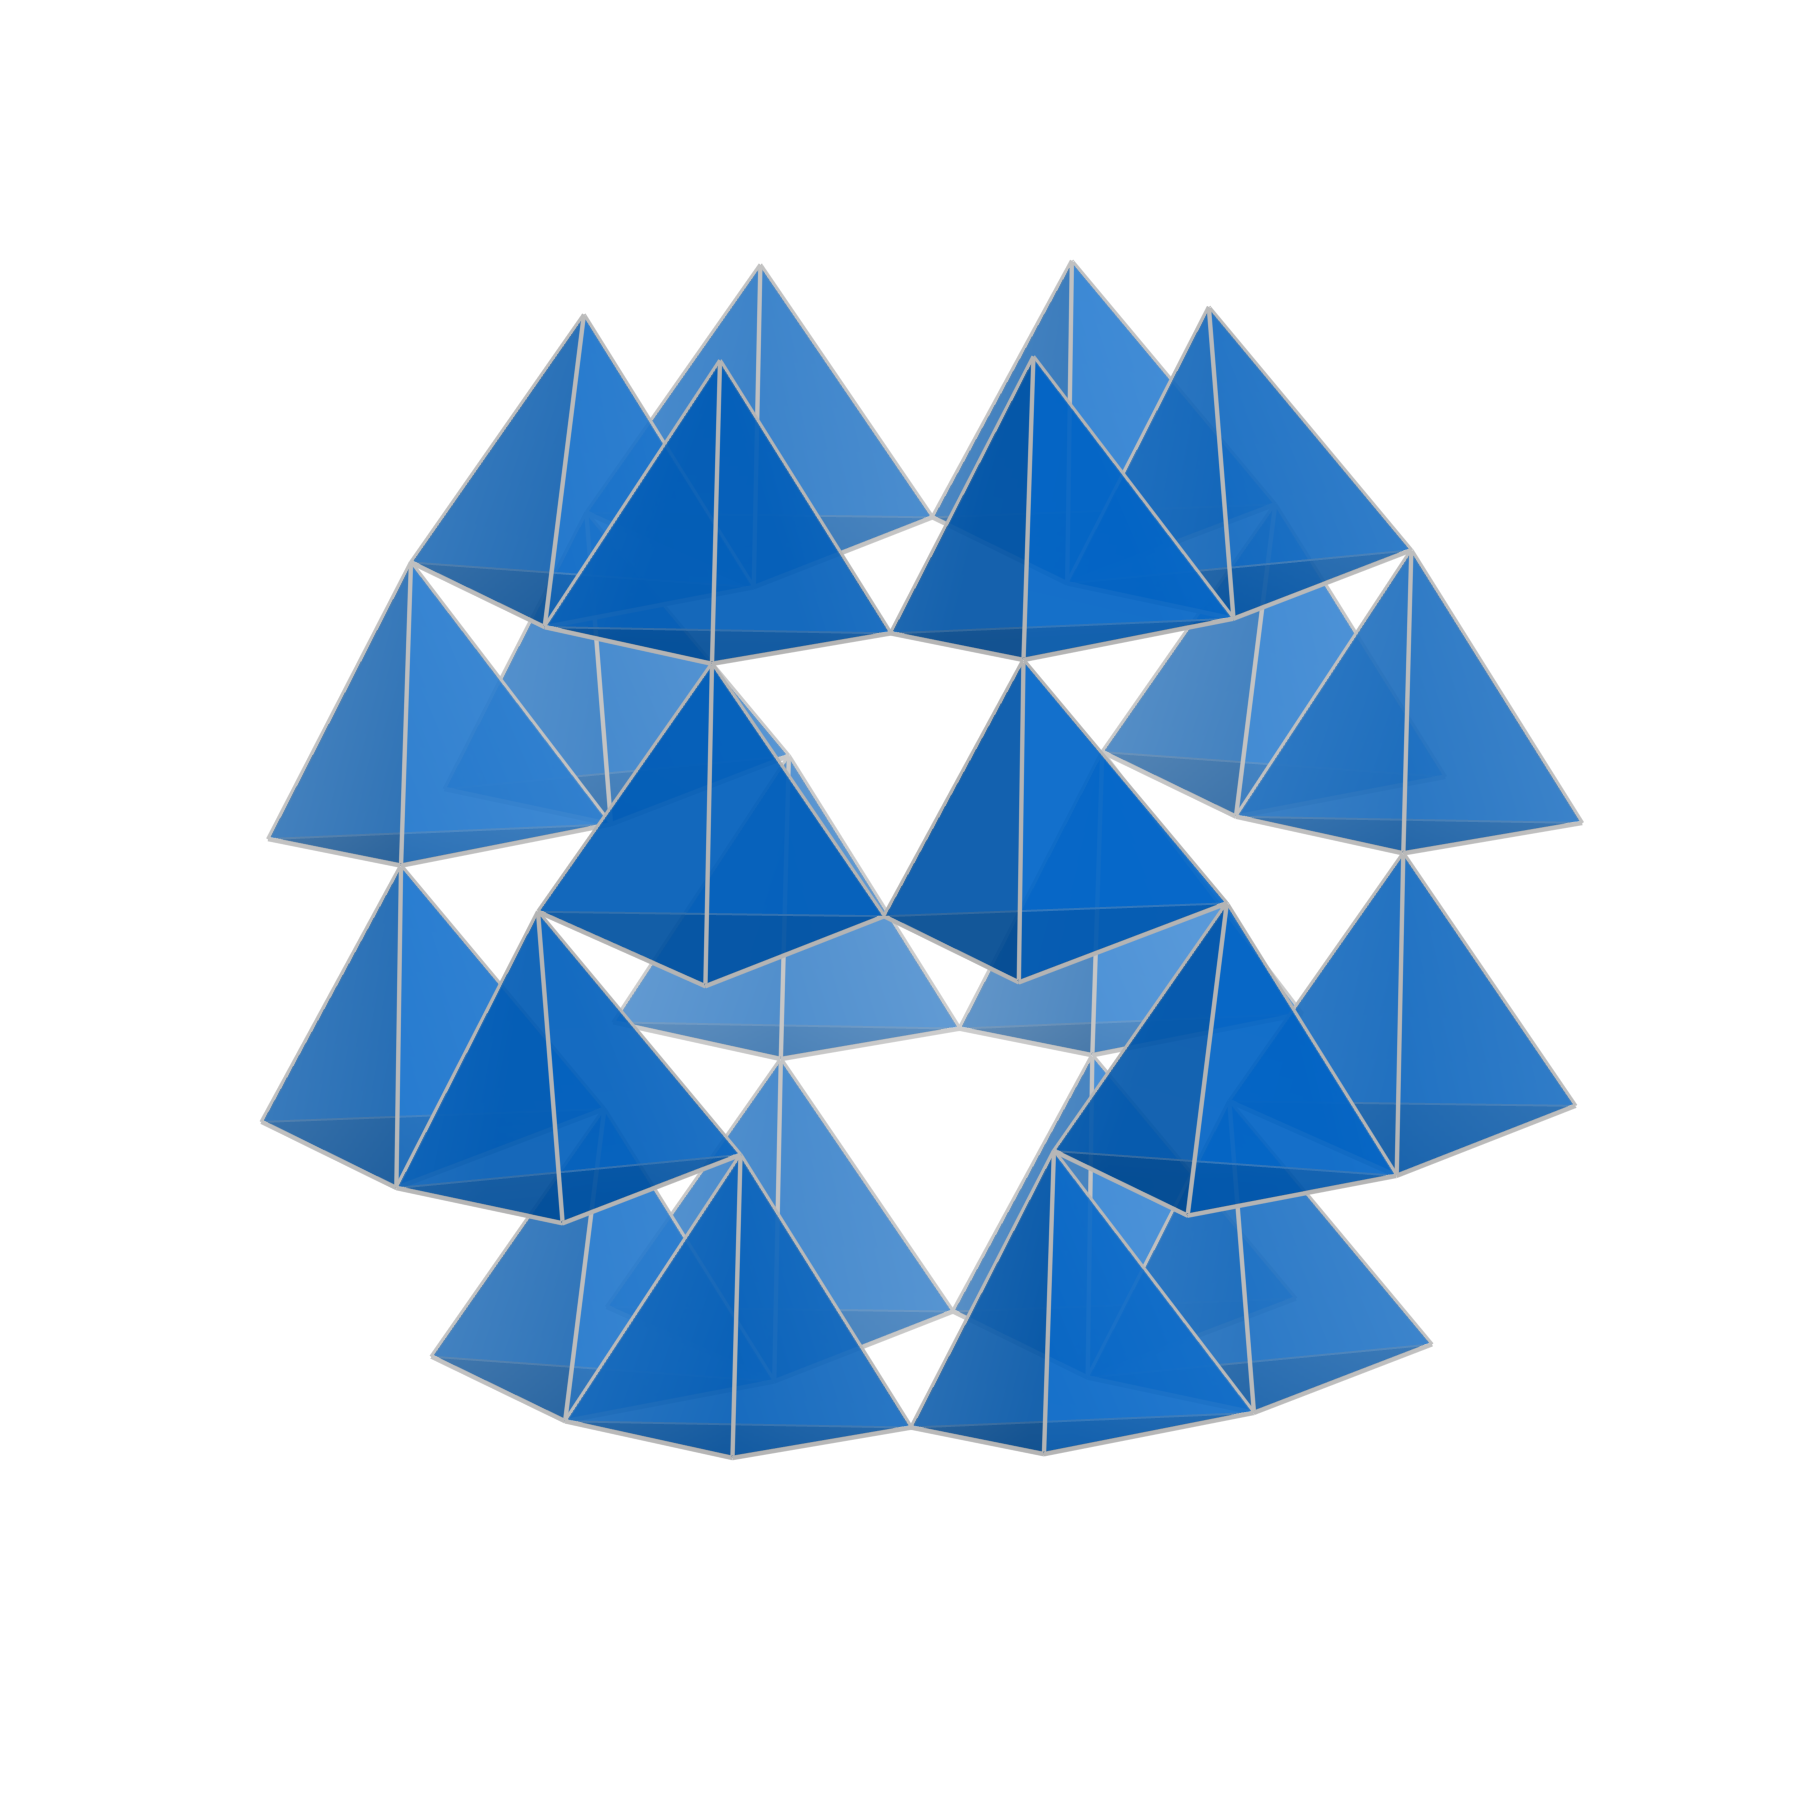
\includegraphics[width=0.9\linewidth]{1_cu12as4s13_crys_st_a} \\ а)
  \end{minipage}
  \hfill
  \begin{minipage}[ht]{0.3\linewidth}\centering
    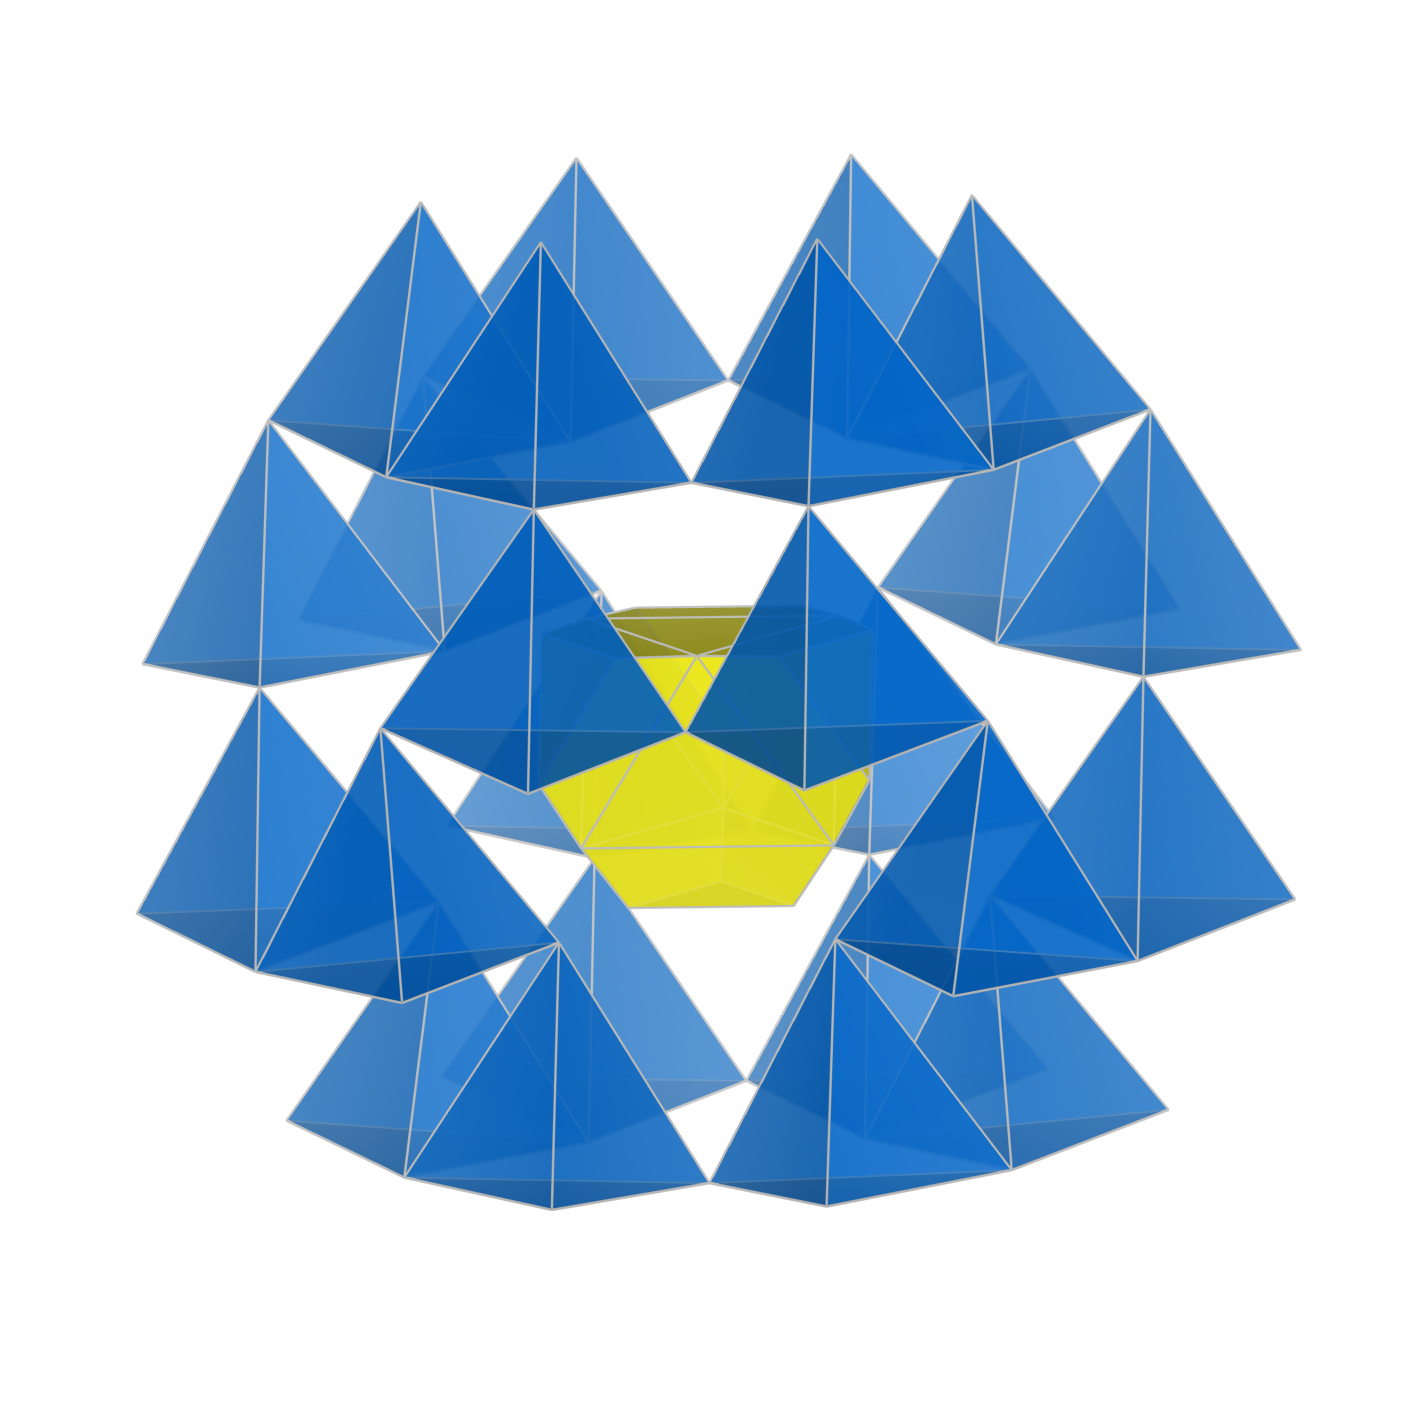
\includegraphics[width=0.9\linewidth]{2_cu12as4s13_crys_st_b} \\ б)
  \end{minipage}
\hfill
 \begin{minipage}[ht]{0.3\linewidth}\centering
    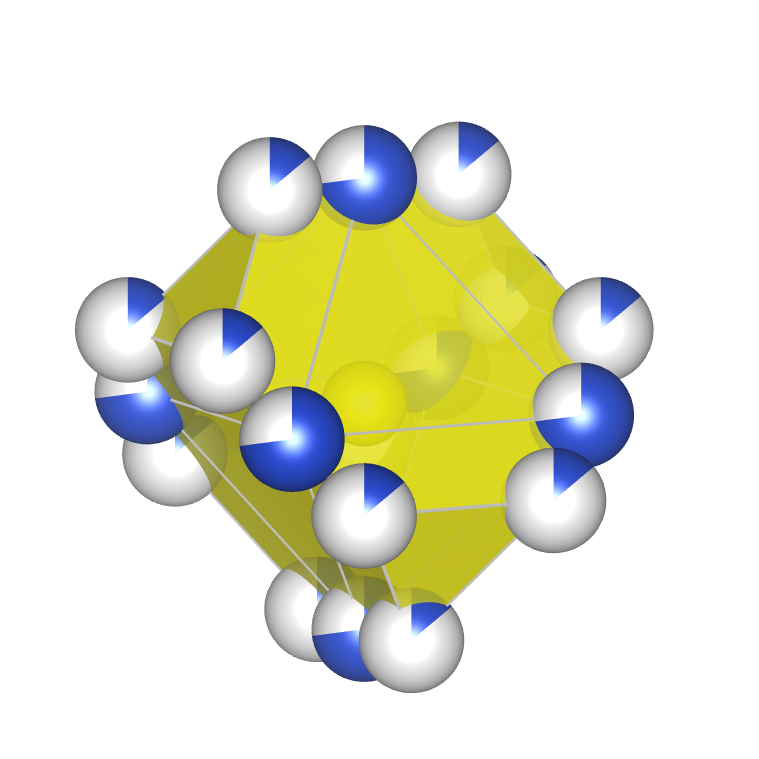
\includegraphics[width=0.9\linewidth]{3_cu12as4s13_crys_st_c} \\ в)
  \end{minipage}
      \caption[Кристаллическая структура халькогенида на примере синтетического теннантита Cu\textsubscript{12}As\textsubscript{4}S\textsubscript{13}]{Кристаллическая структура халькогенида на примере синтетического теннантита Cu\textsubscript{12}As\textsubscript{4}S\textsubscript{13}}
    \label{img:figure1}
\end{figure}

Также в главе дан обзор основных литературных данных о физических свойствах халькогенидов, в частности,  магнитных и транспортных\cite{bab_81}.
По данным \cite{bab_1982,DiBenedetto2002, Bernardini2000,Gainov2008} в структуре возможно возникновение антиферромагнитного упорядочения при понижении температуры. В работах \cite{Lu2013,Lara-Curzio2014,Tablero2014,Lu2016,Nasonova2016} проведены исследования стабильности полиморфных фаз и проанализированы возможности использования соединений в качестве функциональных материалов для термоэлектрических устройств.



Во \underline{\textbf{второй главе}} описаны методики исследования и методы синтеза соединений для систем Cu--As--S, Cu--Sb--S, Cu--As--Se и Cu--Sb--Se в~стехиометрическом соотношении.
А именно: методы порошковой и монокристальной дифрактометрии, измерения и моделирования теплоёмкости, просвечивающей электронной микроскопии, комбинационного рассеяния света и измерения магнитной восприимчивости. Также описаны условия проведения квантовомеханических расчётов.

Соединения Cu\textsubscript{12}V\textsubscript{4}VI\textsubscript{13}, где V = As, Sb и VI = S, Se синтезированы в~кварцевых ампулах с инертной средой. В~качестве исходных материалов использованы реактивы высокой чистоты не ниже марки <<особо чистый>>. Исходная шихта составлена в соотношении 3Cu:1V:3VI
(избыток по~сере или селену составлял не~более 3"--~5~\%). Точность определения температуры в~рабочей камере печи соответствовала 0,5~К при 600~К и 1~К при 1100~К (термопара платина/платина "--- 10~\% родий использовалась для контроля температуры). Синтез проведен в~четыре этапа. Первый~"--- медленное нагревание в~печи (10"--~15~часов) до~температуры, превышающей температуру плавления легколетучего компонента (серы или селена) на~10"--~30~К; второй~"--- поддержание данной температуры 20"--~30~часов. После этого увеличение температуры до~полного плавления образовавшегося в~ампуле вещества в течении 40"--~50~ч. и поддержание этой температуры постоянной 20"--~30 ч. Последний этап"--- понижение температуры до 2/3 от температуры плавления и отжиг соединения 30"--~40~ч. Образец Cu\textsubscript{12}As\textsubscript{4}S\textsubscript{13} после спекания дополнительно был подвергнут направленной перекристаллизации в~двухзонной печи по~методу Стокбаргера"--~Бриджмена. Часть образцов дополнительно была отожженна при~температуре 673 и 773~К в~течении 24~часов.

Исследования образцов проведены методами рентгенофазового и энергодисперсионного анализов.
Рентгенофазовый анализ осуществлен методом порошка на образцах, которые  получены дроблением исходных спеченных образцов до гомогенного состояния в ступке. Дифрактограммы  обрабатывались в~программном комплексе Jade~6 с использованием реферативной базы pdf2. Полученные образцы аттестованы на порошковом дифрактометре D8 Advance (Bruker, Германия) на Cu K$\alpha$ излучении. Три соединения из синтезированных  идентифицированы в кубической сингонии, одно --- в~тетрагональной cингонии.

Прецизионное исследование структуры монокристалла теннантита проведено на четырехкружном автоматическом дифрактометре Xcalibur c 2d детектором  CCD~EOS~S2 и с~системой охлаждения Cobra Plus при температурах 85, 115, 180, 250 и 293~K.
В работе исследовались сколы от монокристаллического образца с линейными размерами от 100 до 300~мкм.
Температурные эксперименты проведены с использованием характеристического Mo K\textsubscript{$\alpha$} изучения с длиной волны 0.71073~$\angstrom$. Дополнительно было проведено исследование структуры образца сферической формы синтетического теннантита при комнатной температуре.

Изображения атомных структур получены на электронном микроскопе FEI Titan 80--300 в режиме HAADF-STEM  при ускоряющем напряжении 300 кВ.
HAADF режим дает контраст по атомному номеру (зависимость Z\textsuperscript{2}).
Образец приготовлен с помощью системы фокусированного ионного пучка (FIB) на двухлучевом сканирующем микроскопе "--- FEI Helios 600.
Изображения получены при комнатной температуре на ламельке толщиной менее 100~нм и плоскости синтетического теннантита (011) Cu\textsubscript{12}As\textsubscript{4}S\textsubscript{13}.
Обработка изображений произведена в программном обеспечении atomap\cite{Nord2017}. С помощью программного обеспечения было проведено определение колонок атомов меди и их эллиптичности. Дополнительно был учтен дрейф и получены изображения, показывающие величину эллиптичности для рядов атомов меди в плоскости (011).

Теплоёмкость измерена при помощи измерительного комплекса PPMS (Quantum Design,
США) в диапазоне температур от 2 до 350 К. Измерения проводились методом релаксации теплового импульса\cite{Hwang_1997}. Измерительный комплекс представляет собой автономный комплекс с гелиевым криостатом замкнутого цикла. Расчётная кривая теплоёмкости получена вычислением функции Дебая с тремя дополнительными осцилляторами Эйнштейна. Выбор характеристических температур осцилляторов Эйнштейна описан в тексте диссертации. Добавление осцилляторов Эйнштейна рассматривается в описании экспериментальных данных и обуславливается смягчением фононных мод в соединениях.

Квантовомеханические вычисления проводились в рамках теории функционала плотности с использованием программы VASP (Vienna Ab initio Simulation Package) \cite{Kresse1993,Kresse1994,Kresse1996}, основанной на методе присоединённых плоских волн. Равновесная атомная геометрия зоны Бриллюэна была разбита  на 7~k"~точек с помощью метода Монкхоста--Пака (Monkhorst--Pack) \cite{Monkhorst_1976}. Величина энергии обрезания в расчёте равнялась 300~эВ. Оптимизация атомной структуры проводилась до тех пор, пока межатомные силы не становились меньше 0.005~эВ/${\angstrom}$.

Спектры комбинационного рассеяния получены на спектрометре TRIAX-552, оборудованном охлаждаемым детектором Peltier TE CCD SPEC 10 (Princeton Instruments).
Была использована решетка 600 штрихов на мм и 50-кратная линза Mitutoyo M Plan Apo SL50 (числовая апертура 0.42).
Для возбуждения спектров комбинационного рассеяния применен аргон-ионный лазер с длиной волны 514.5~нм Spectra-Physics Stabilite 2017 с выходной мощностью от 0.3 до 1~мВт на образце. Калибровка проведена с использованием линии спектра комбинационного рассеяния света 520.5~см\textsuperscript{-1} полированной кремниевой пластины и/или линий спектра комбинационного рассеяния неона.
Для получения спектра комбинационного рассеяния вблизи возбуждающей линии в оптической схеме были использованы 3  брэгговских фильтра.

Магнитные свойства образцов измерены с
помощью магнитоизмерительного комплекса
MPMS--XL7~EC (Quantum Design, США) с первичным преобразователем на основе СКВИДа в~диапазоне температур от 2 до 350 К и в постоянных магнитных полях напряженностью до 70 кЭ. Шаг измерения в диапазоне от $-$5 до 5~кЭ составляет 0.1~Э, при больших полях "--- 1~Э.

В \underline{\textbf{третьей главе}} представлены результаты исследования монокристаллического образца синтетического теннантита Cu\textsubscript{12}As\textsubscript{4}S\textsubscript{13} методами монокристальной дифрактометрии в диапазоне температур от 85 до 293~К, просвечивающей микроскопии монокристаллического образца в плоскости (011) и моделирования структур теннантита с разным расположением атомов в лавесовском полиэдре методом первопринципных расчётов.



Исследование монокристаллического образца  Cu\textsubscript{12}As\textsubscript{4}S\textsubscript{13} проведено при температурах 85, 115, 180, 250 и 293~К. Образцы получены сколом от монокристаллического образца с линейными размерами от 100 до 300~мкм.  Результаты дифракционных экспериментов при разных температурах представлены в таблице~\ref{xray1}. С понижением температуры объем элементарной ячейки ожидаемо уменьшается и возрастает значение R-фактора, a  заселенность позиции Cu2 (pис.~\ref{img:figure1}в) возрастает и  наблюдается аномальное изменение значения коэффициента атомарного смещения для позиции S2 (pис.~\ref{img:figure1}в), которое показывает наличие фазового перехода второго рода в диапазоне от 115 до 180 К.



\begin{landscape}
\begin{table} [htbp]
\centering
\caption{Сводная таблица данных рентгеноструктурных исследований для синтетического теннантита Cu\textsubscript{12}As\textsubscript{4}S\textsubscript{13} при температурах 85, 115, 180, 250 и 293~К}%
	\label{xray1}% label всегда желательно идти после caption
    \renewcommand{\arraystretch}{1.5}
	\begin{tabular}{@{}@{\extracolsep{20pt}}llllll@{}}
 \toprule     %%% верхняя линейка
T, K                       & 85          & 115         & 180         & 250         & 293         \\
   \midrule
a, $\angstrom$                       & 10.1439(2)  & 10.1446(2)  & 10.1463(2)  & 10.1523(2)  & 10.1572(2)  \\ \hline
V, $\angstrom^3$                      & 1043.79(4)      & 1044.01(4)      & 1044.54(4)      & 1046.39(4)      & 1047.91(4)      \\ \hline
Группа симметрии                     &\multicolumn{5}{c}{ I–43m  }                                         \\ \hline
Длина волны, ($\angstrom$) & \multicolumn{5}{c}{Mo K\textsubscript{$\alpha$}, 0.71069 } \\ \hline
Дифрактометр             & \multicolumn{5}{c}{Xcalibur}                                       \\ \hline
Коррекция абсорбции      & \multicolumn{5}{c}{аналитическая(по форме кристалла)} \\ \hline
$\theta_{max}$,\textsuperscript{ $\circ$ }                 &  \multicolumn{5}{c}{42.08 } \\ \hline
R\textsubscript{int}                       & 0.052       & 0.054       & 0.049       & 0.050       & 0.049       \\ \hline
N\textsubscript{ref} , регистрированный           & 11028       & 11029       & 11036       & 11010       & 11026       \\ \hline
I $\geq \sigma$(I)                  & 693         & 691         & 686         & 677         & 667         \\ \hline
N\textsubscript{paf}                       & 36          & 42          & 47          & 47          & 44          \\ \hline
GOF                        & 1.06        & 1.15        & 1.03        & 1.01        & 1.00        \\ \hline
R/R\textsubscript{w}                     & 0.034/0.052 & 0.037/0.056 & 0.031/0.045 & 0.032/0.045 & 0.029/0.038 \\ \hline
$\pm\Delta\rho   $                     & +2.9/–1.8   & +3.5/–1.7   & +2.3/–1.1   & +1.8/–1.1   & +1.7/–1.2   \\ \hline
R\textsubscript{MEM}                     & 0.017/0.021 & 0.016/0.021 & 0.018/0.022 & 0.018/0.022 & 0.019/0.021\\ \hline
 \bottomrule
\end{tabular}
\end{table}
\end{landscape}


Анализ изображения структуры показывает наличие распределенной электронной плотности в форме эллипса у некоторых рядов и косвенно подтверждает наличие сдвинутых атомов меди в структуре теннантита. На рисунке \ref{img:figure5}в) представлены атомарные ряды меди, которые имеют форму эллипса, с учётом дрейфа для плоскости (011) синтетического теннантита Cu\textsubscript{12}As\textsubscript{4}S\textsubscript{13}.


\begin{figure}[ht]
  \begin{minipage}[ht]{0.3\linewidth}\centering
    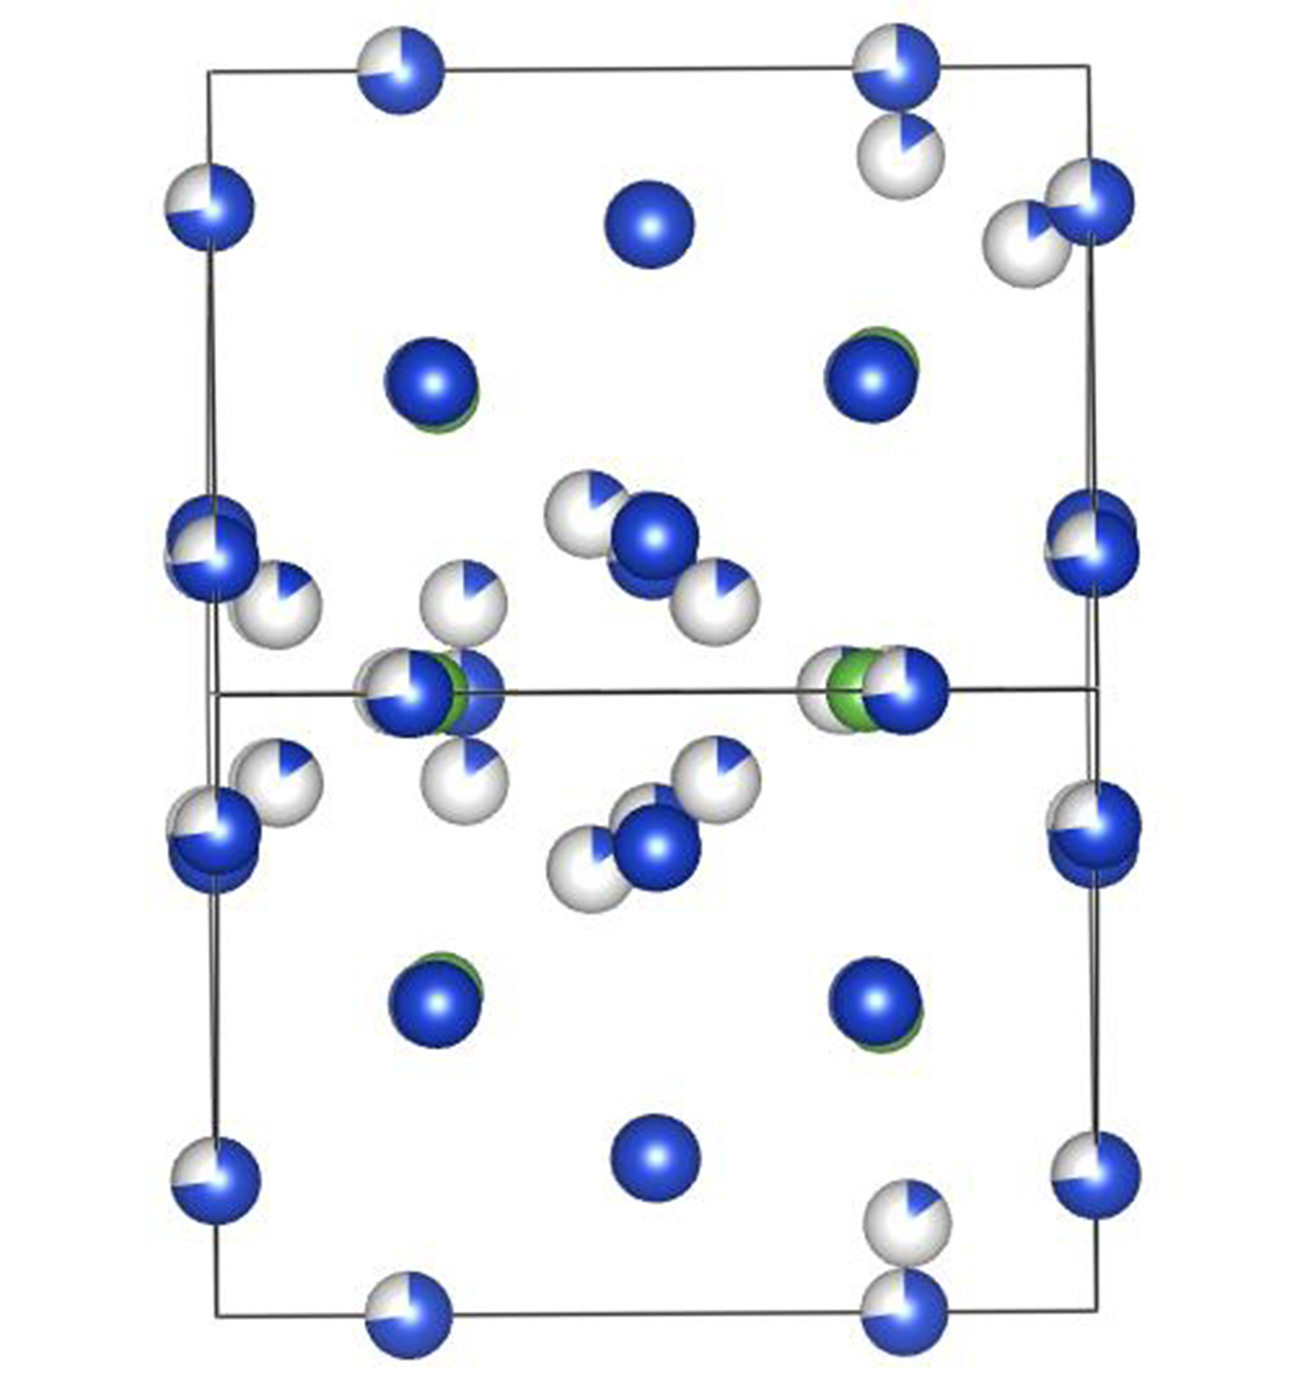
\includegraphics[width=0.9\linewidth]{mic_cu12as4s13_110_a} \\ а)
  \end{minipage}
  \hfill
  \begin{minipage}[ht]{0.3\linewidth}\centering
    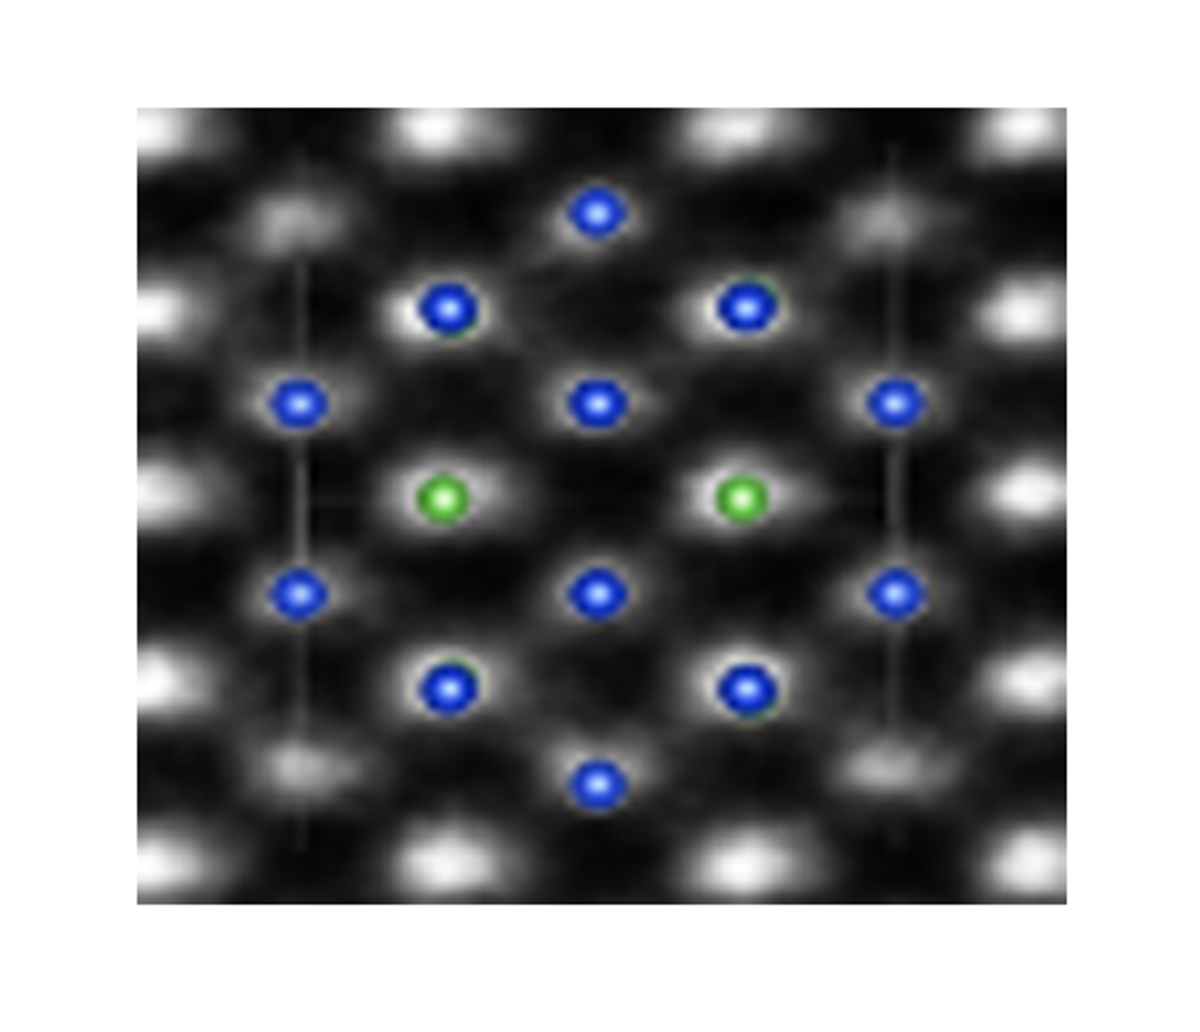
\includegraphics[width=0.9\linewidth]{mic_cu12as4s13_110_b} \\ б)
  \end{minipage}
  \hfill
  \begin{minipage}[ht]{0.3\linewidth}\centering
    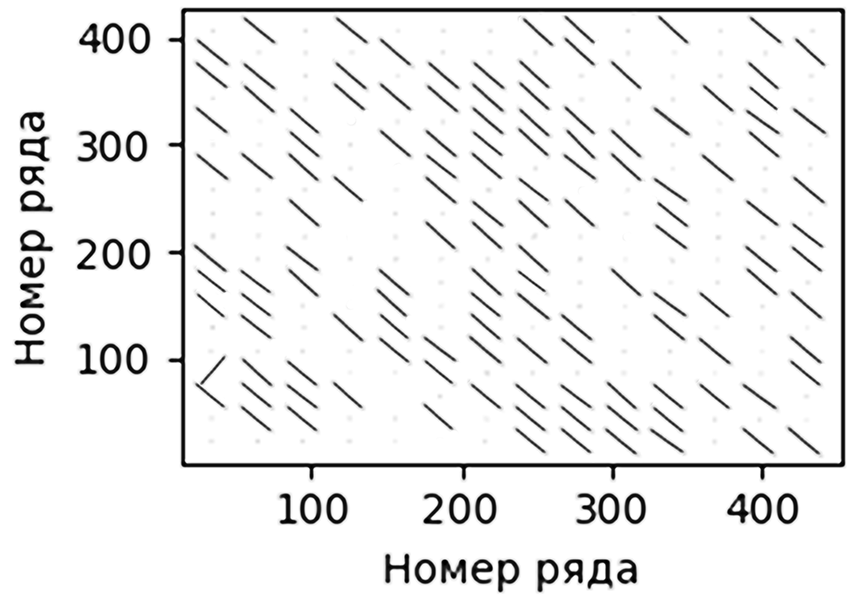
\includegraphics[width=0.9\linewidth]{mic_cupper_raw} \\ в)
  \end{minipage}
      \caption[Изображение расположения атомных рядов (синим обозначен атом меди, зеленым --- мышьяка) для синтетического теннантита Cu\textsubscript{12}As\textsubscript{4}S\textsubscript{13} в плоскости (011) (а), совмещенное изображение экспериментального изображения и атомарных рядов для синтетического теннантита Cu\textsubscript{12}As\textsubscript{4}S\textsubscript{13} в плоскости (011) (б),  изображение  рядов для атомов меди, в которых электронная плотность имеет форму эллипса и полученная после анализа атомарного изображения эллиптичность для рядов меди синтетического теннантита Cu\textsubscript{12}As\textsubscript{4}S\textsubscript{13} (в)]{Изображение расположения атомных рядов (синим обозначен атом меди, зеленым --- мышьяка) для синтетического теннантита Cu\textsubscript{12}As\textsubscript{4}S\textsubscript{13} в плоскости (011) (а), совмещенное изображение экспериментального изображения и атомарных рядов для синтетического теннантита Cu\textsubscript{12}As\textsubscript{4}S\textsubscript{13} в плоскости (011) (б),  изображение  рядов для атомов меди, в которых электронная плотность имеет форму эллипса и полученная после анализа атомарного изображения эллиптичность для рядов меди синтетического теннантита Cu\textsubscript{12}As\textsubscript{4}S\textsubscript{13} (в)}
    \label{img:figure5}
\end{figure}


Для исследования наиболее выгодного положения атомов меди были рассчитаны энергии 20 структур с разным положением атомов меди.
Структуры разделены на две группы: первая --- в лавесовском полиэдре сдвинуты 6 атомов меди (структуры с 1 по 10), вторая --- сдвинуты 3 атома меди в лавесовском полиэдре (структуры с 10 по 19).
На рисунке \ref{img:th} представлен график со значениями энергий элементарных ячеек для рассчитанных структур. Красной пунктирной линией обозначена энергия исходной структуры.
Экспериментальные структуры, полученные после анализа рентгеноструктурных данных  экспериментов при разных температурах, были рассчитаны с учетом ферромагнитного (ФМ), антиферромагнитного (АФМ), парамагнитного (ПМ) и диамагнитного состояний в структурах. 
Антиферромагнитное упорядочение в экспериментальной структуре при 85~К энергетически более выгодно, чем ферро-, пара- или диамагнитное состояния. При этом для 293~К ФМ, АФМ, ПМ конфигурации имеют одинаковую до (4 знака) энергию, что указывает на их одинаковую вероятность.

\begin{figure}[ht]
  \begin{minipage}[ht]{0.9\linewidth}\centering
    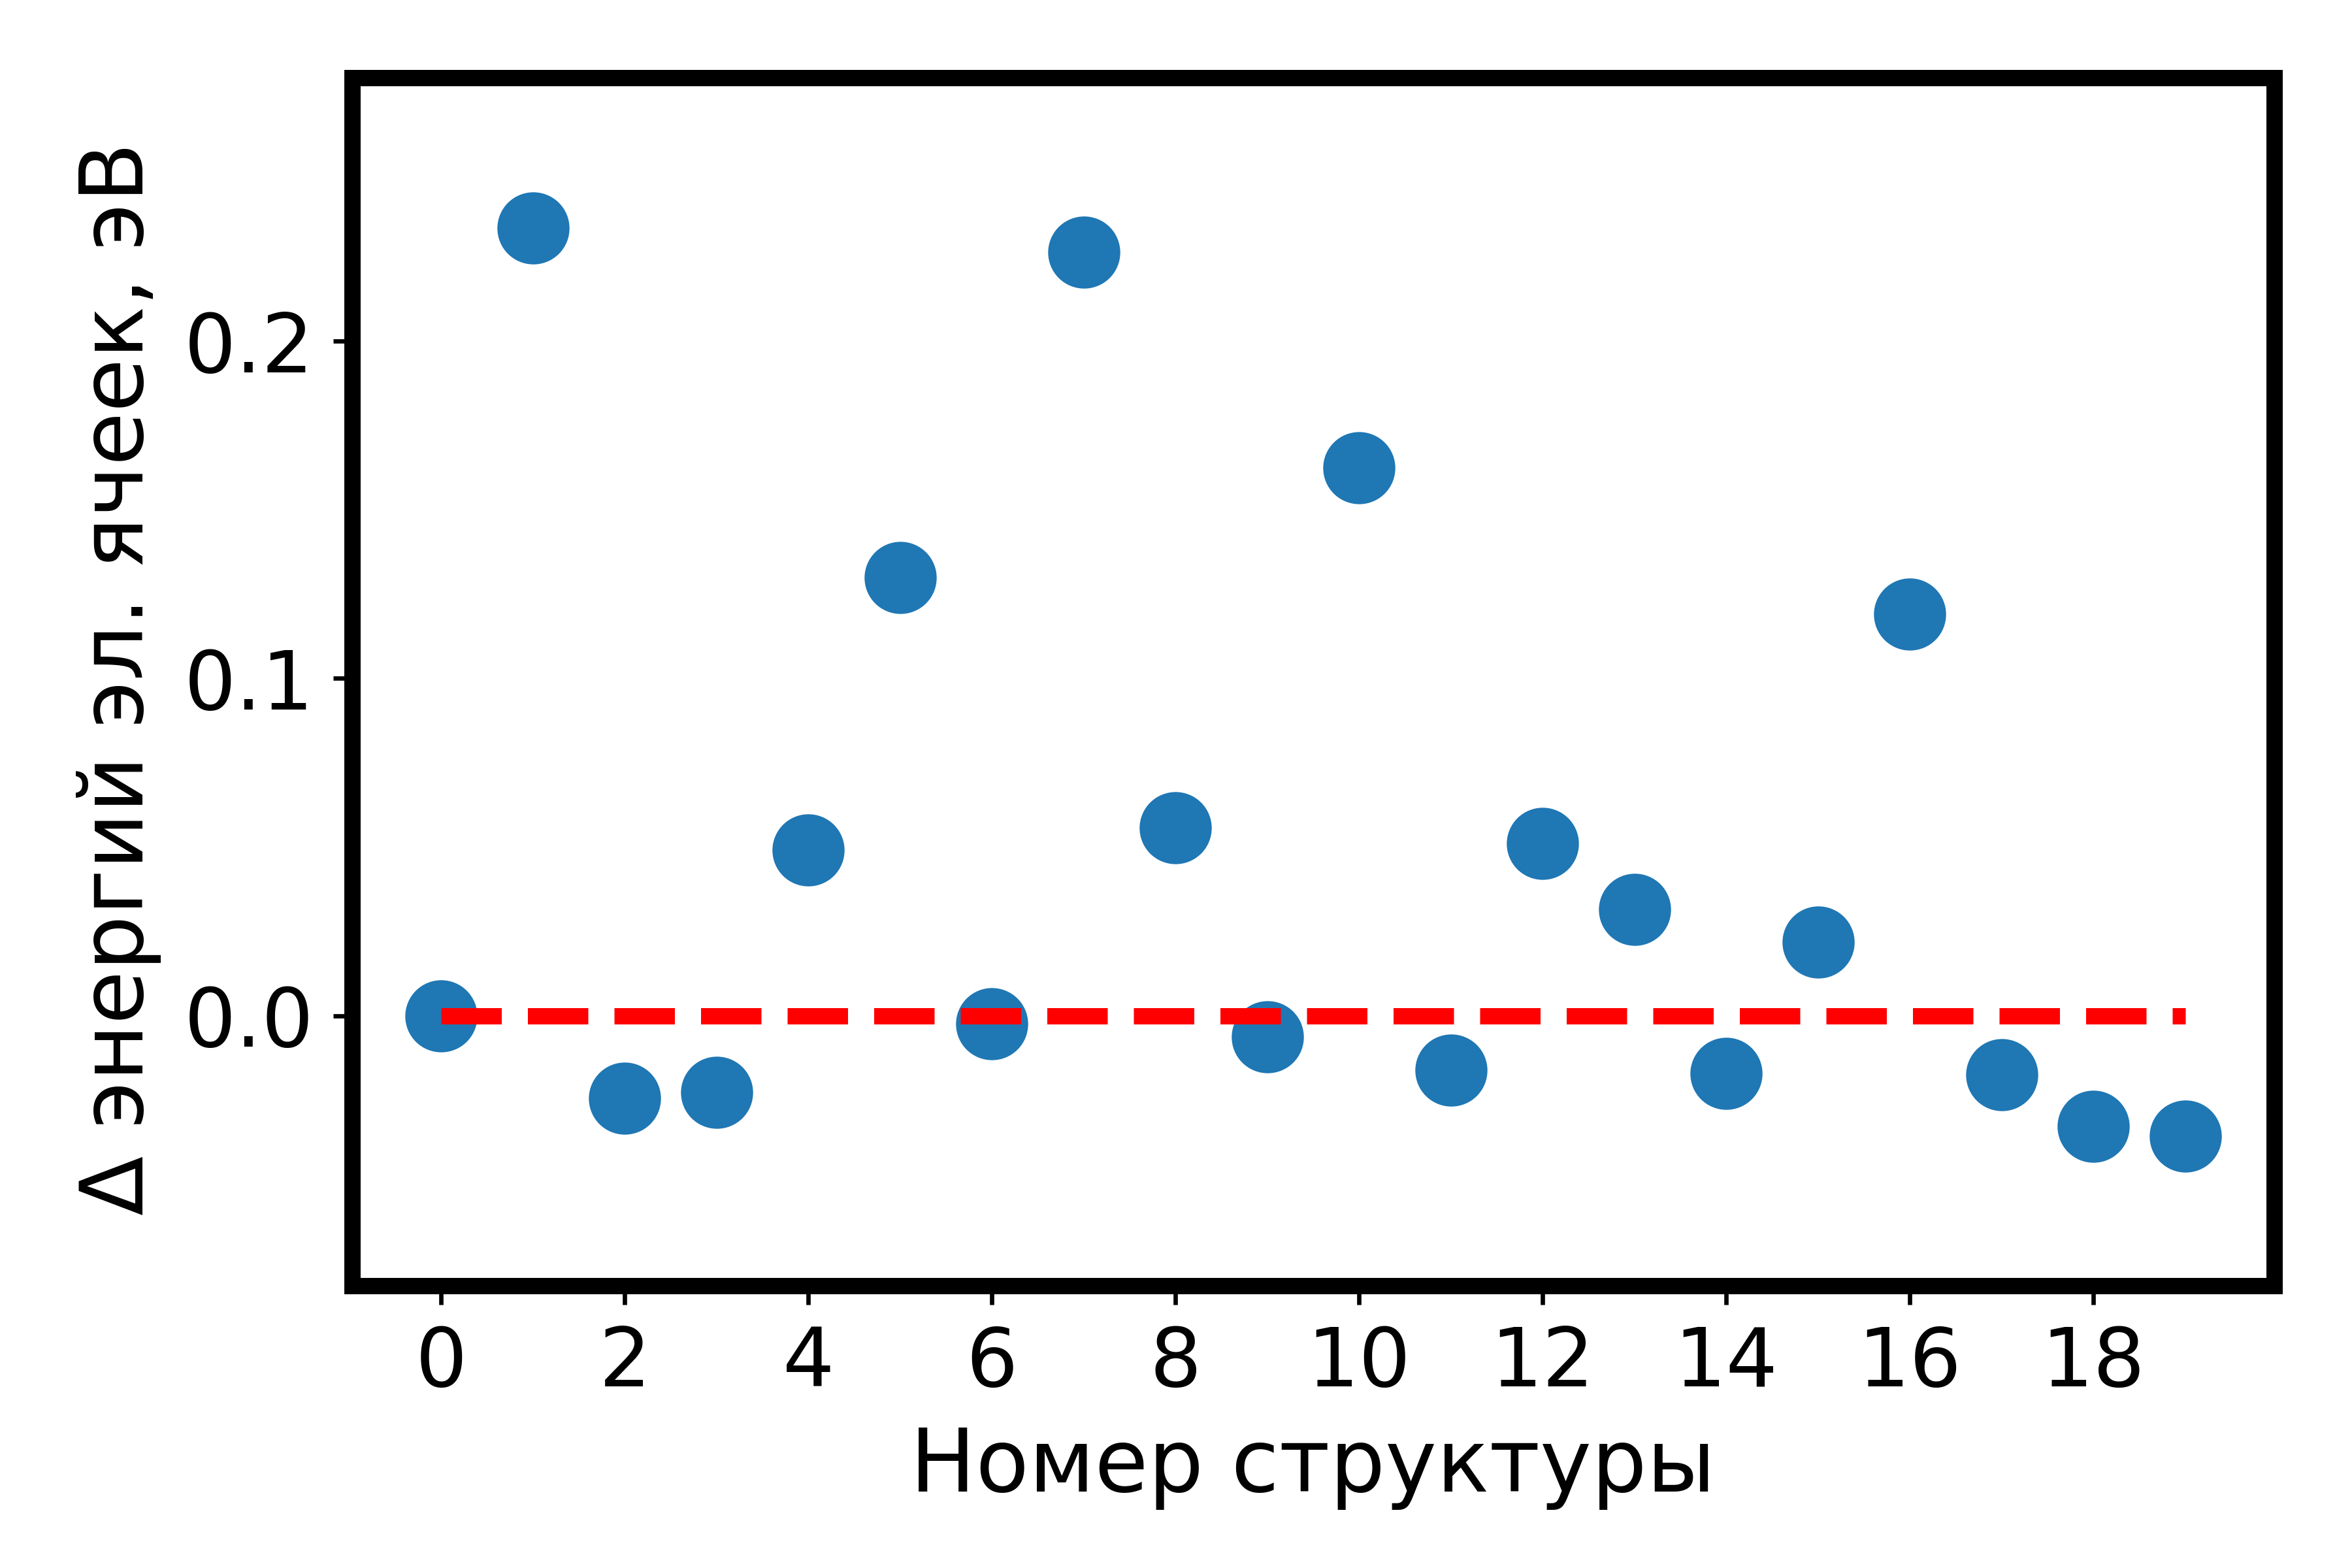
\includegraphics[width=0.7\linewidth]{energy_structure}
  \end{minipage}

      \caption[Сводный график энергий рассчитанных структур относительно энергии исходной структуры с разным расположением атомов в лавесовском полиэдре]{Сводный график энергий рассчитанных структур относительно энергии исходной структуры с разным расположением атомов в лавесовском полиэдре}
    \label{img:th}
\end{figure}

По результатам рентгеноструктурного анализа монокристаллического образца синтетического теннантита Cu\textsubscript{12}As\textsubscript{4}S\textsubscript{13} при комнатной температуре обнаружено, что значение суммы заселенностей позиций атомов Cu2 и Cu21 составляет 1, а не 1.04 как опубликовано ранее\cite{Makovicky_2006}.
Полученные результаты показывают, что на структурную формулу синтетического теннантита приходится 12 атомов меди, а не 12.5.
Таким образом, лавесовский полиэдр состоит из 6 атомов меди.
Наличие рядов меди с электронной плотностью в форме эллипса, определенное после анализа плоскости (011) атомарного изображения монокристаллического образца синтетического теннантита Cu\textsubscript{12}As\textsubscript{4}S\textsubscript{13} (Рис.~\ref{img:figure5}), показывает существование позиции атома меди Cu21 и согласуется с результатами рентгеноструктурного анализа, описанного выше.

По данным первопринципных расчётов энергий элементарных ячеек для синтетического теннантита Cu\textsubscript{12}As\textsubscript{4}S\textsubscript{13} следует,  что смещение атома меди в лавесовском полиэдре может приводить как к увеличению энергии ячейки, так и к уменьшению.
Результаты показывают, что существующее неэквивалентное  окружение атомов меди в позициях Cu21 и Cu2 ведет к отличию химического потенциала для структур с разным расположением атомов меди (анализировались позиции Cu21 и Cu2) и, вероятно, является движущей силой для возникновения позиции Cu21. Расстояние между сдвинутым атомом и его идеальным положением в лавесовском полиэдре составляет для наиболее энергетически выгодной элементарной ячейки 0.6~$\angstrom$, по экспериментальным данным --- 1.027(6)~$\angstrom$.
Анализ распределения электрических зарядов показывает, что для более выгодных с энергетической точки зрения структур не возникает разной валентности на атомах меди Cu1,
но появляется разность зарядов для позиций атомов Cu2 (Cu21) (варианты структур с 11 по 15). Также следует отметить, что структуры, где сдвинуты все 6 атомов меди, обладают большей энергией элементарной ячейки в сравнении с энергией идеального полиэдра и имеют не самые энергетически выгодные конфигурации  (варианты 5--10).

На рисунке \ref{img:xray2} показаны изображения распределений электронной плотности синтетического теннантита Cu\textsubscript{12}As\textsubscript{4}S\textsubscript{13} при температуре 293~(а) и 85~(б)~К в плоскости (011).
По форме сечений линий электронной плотности видно, что происходит полное разделение позиций Cu2 и Cu21.
При комнатной температуре расстояние между Cu2 и Cu21 составляет 1.027(6)~$\angstrom$, при 85~К --- 1.108(5)~$\angstrom$.
Расчёт энергий ФМ, АФМ, ПМ и диамагнитного состояний для экспериментально полученных структур показывает, что АФМ упорядочение в экспериментальной структуре при 85~К энергетически более выгодно, чем ферро-, пара- или диамагнитное состояния при этой же температуре.
Для экспериментальной структуры при 293~К ФМ, АФМ, ПМ конфигурации имеют одинаковую до (4 знака) энергию, что указывает на их одинаковую вероятность.

\begin{figure}[hb]
  \begin{minipage}[ht]{0.5\linewidth}\centering
    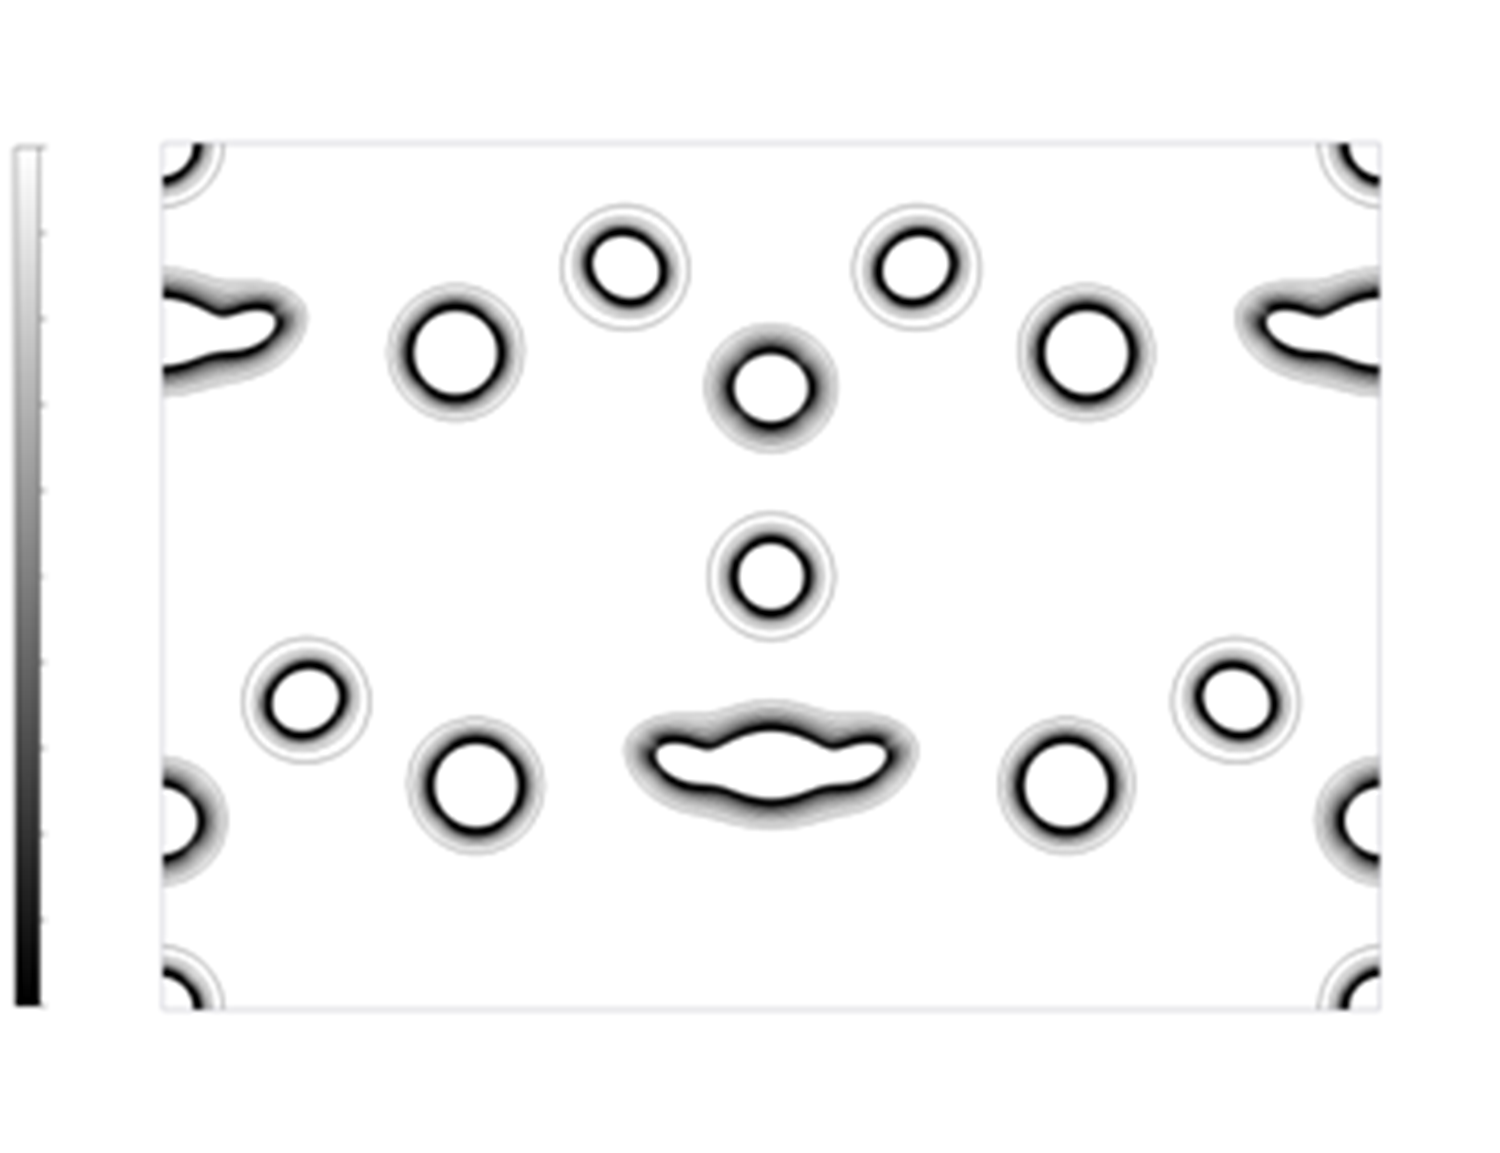
\includegraphics[width=0.9\linewidth]{Electron_density_293.png} \\ а)
  \end{minipage}
  \hfill
  \begin{minipage}[ht]{0.5\linewidth}\centering
    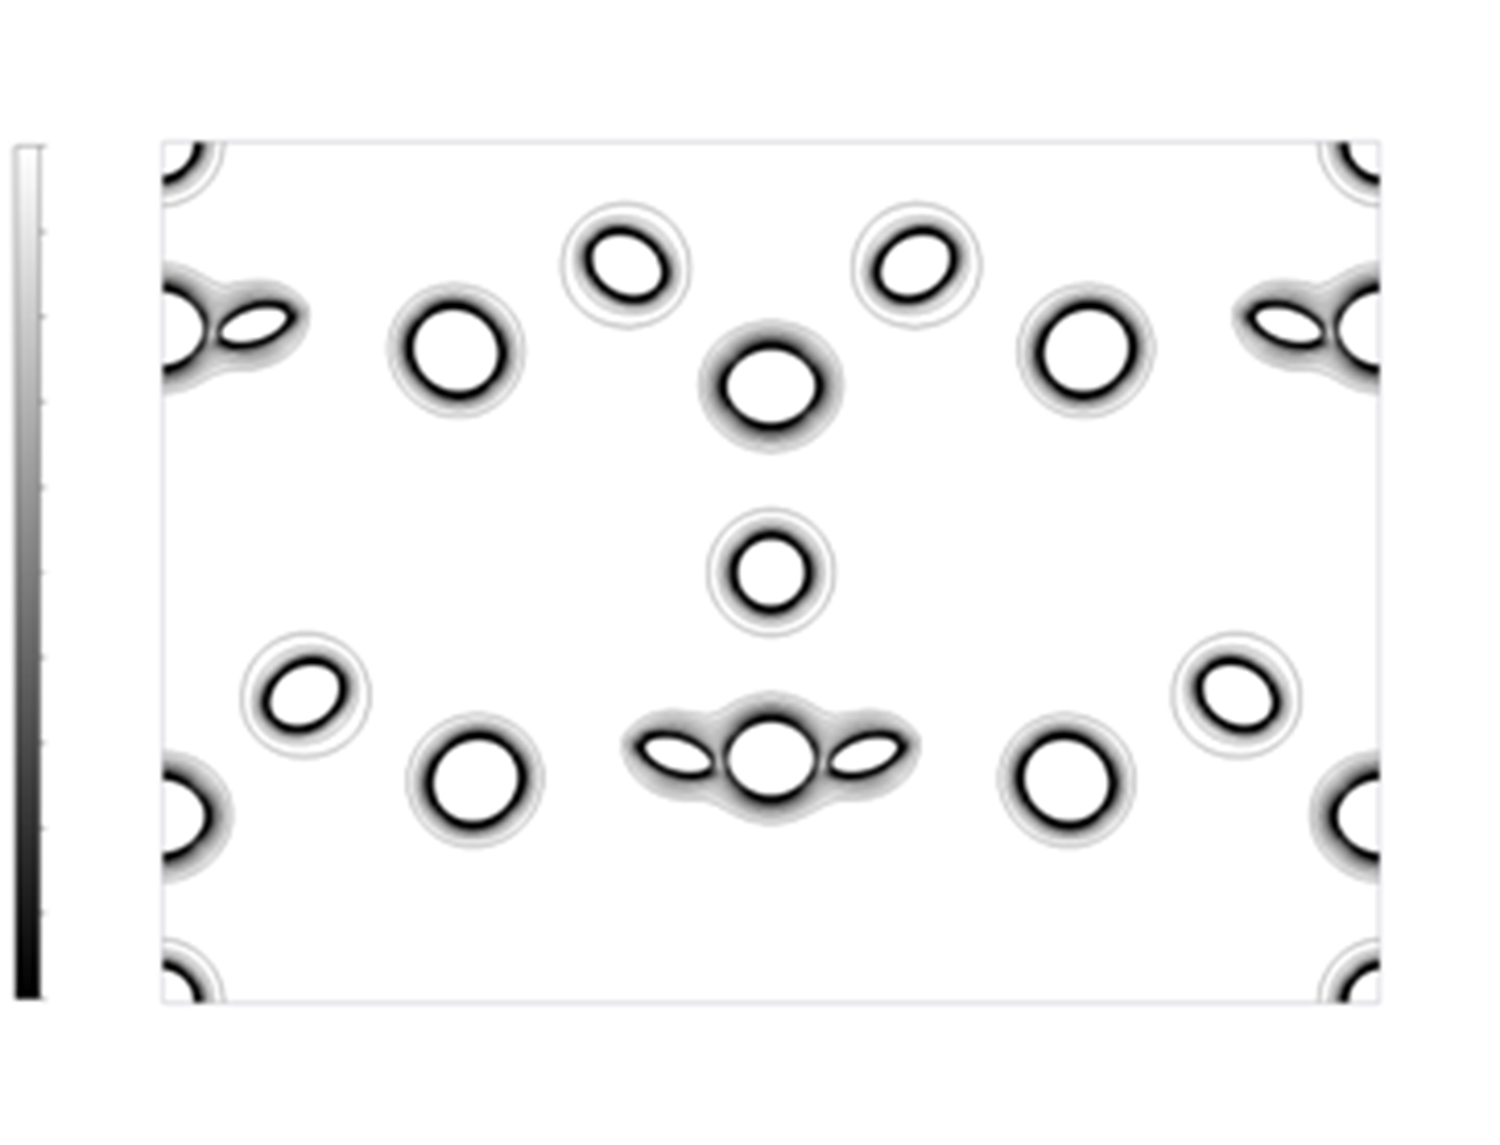
\includegraphics[width=0.9\linewidth]{Electron_density_85.png} \\ б)
  \end{minipage}

      \caption[Распределение электронной плотности при температуре 293~(а) и 85~(б)~К в плоскости (011) синтетического теннантита Cu\textsubscript{12}As\textsubscript{4}S\textsubscript{13}]{Распределение электронной плотности при температуре 293~(а) и 85~(б)~К в плоскости (011) синтетического теннантита Cu\textsubscript{12}As\textsubscript{4}S\textsubscript{13}}
    \label{img:xray2}
\end{figure}

В \underline{\textbf{четвёртой главе}} представлены результаты экспериментальных исследований зависимостей намагниченности в диапазоне температур от 2 до 350~К и спектров комбинационного рассеяния света для соединений Cu\textsubscript{12}As\textsubscript{4}S\textsubscript{13}, Cu\textsubscript{12}Sb\textsubscript{4}S\textsubscript{13}, Cu\textsubscript{3}AsSe\textsubscript{3} и Cu\textsubscript{3}SbSe\textsubscript{3} при комнатной температуре. А также измерения теплоёмкости в диапазоне температур от 4 до 350~К и результаты моделирования теплоёмкости для Cu\textsubscript{12}As\textsubscript{4}S\textsubscript{13} и Cu\textsubscript{3}AsSe\textsubscript{3}.

На рисунке \ref{img:figure4} представлены результаты расчётной и экспериментальной температурных зависимостей для синтетических теннантита Cu\textsubscript{12}As\textsubscript{4}S\textsubscript{13} и мгриита Cu\textsubscript{3}AsSe\textsubscript{3}.

 Температура Дебая при вычислении теплоёмкости для синтетического теннантита Cu\textsubscript{12}As\textsubscript{4}S\textsubscript{13} принята $\theta$\textsubscript{д}~=~623~К на основе лучшего соответсвия расчетной  и экспериментальной  теплоёмкостей. Значения характеристических температур для осцилляторов Эйнштейна составляют $\theta$\textsubscript{э1}~=~220~К, $\theta$\textsubscript{э2}~=~124~К и $\theta$\textsubscript{э3}~=~41~К.
Температура Дебая при вычислении теплоёмкости для синтетического мгриита принята Cu\textsubscript{3}AsSe\textsubscript{3} $\theta$\textsubscript{д}~=~500~К  на основе лучшего соответсвия расчетной  и экспериментальной  теплоёмкостей. Значения для осцилляторов Эйнштейна составляют $\theta$\textsubscript{э1}~=~290~К, $\theta$\textsubscript{э2}~=~185~К и $\theta$\textsubscript{э3}~=~44 К, которые определены из температурных зависимостей удельной намагниченности и литературных данных.

\begin{figure}[ht]
  \begin{minipage}[ht]{0.5\linewidth}\centering
    \includegraphics[width=0.9\linewidth]{Heat_capacity_Cu12As4S13} \\ а)
  \end{minipage}
  \hfill
  \begin{minipage}[ht]{0.5\linewidth}\centering
    \includegraphics[width=0.9\linewidth]{Heat_capacity_Cu3AsSe3} \\ б)
  \end{minipage}

      \caption[Зависимость теплоёмкости образцов Cu\textsubscript{12}As\textsubscript{4}S\textsubscript{13}(а) и Cu\textsubscript{3}AsS\textsubscript{3}(б) от температуры. Точки~"---экспериментальные данные, сплошная линия~"---модельные значения теплоёмкости, пунктиром отмечен уровень доверия 95\% ]{Зависимость теплоёмкости образцов Cu\textsubscript{12}As\textsubscript{4}S\textsubscript{13}(а) и Cu\textsubscript{3}AsS\textsubscript{3}(б) от температуры. Точки~"---экспериментальные данные, сплошная линия~"---модельные значения теплоёмкости, пунктиром отмечен уровень доверия 95\%}
    \label{img:figure4}
\end{figure}

Спектры комбинационного рассеяния для исследованных соединений обладают низкоэнергетическими модами (Рис. \ref{img:figure_raman}).
В таблице \ref{tabl_raman} представлены определенные по экспериментальным спектрам положения пиков для исследуемых соединений и их полуширина.
Следует отметить, что энергия пиков для соединения Cu\textsubscript{12}Sb\textsubscript{4}S\textsubscript{13} составляет 8.5  и 12~мэВ, что наxодится в хорошем согласии с опубликованными теоретическими\cite{Lai_2015} и экспериментальными\cite{May2016}  данными.

Определение положения  и  полуширины пика проведены с помощью функции псевдо-Фойгта.
Модель аппроксимации  основана на функциях псевдо-Фойгта для каждого пика и полиномной функции для фона.

\begin{table} [t!]%
    \centering
	\caption{Положение пиков на спектрах комбинационного рассеяния и их полуширина для сложных соединений халькогенидов меди}%
	\label{tabl_raman}% label всегда желательно идти после caption
    \renewcommand{\arraystretch}{1.5}
	\begin{tabular}{@{}@{\extracolsep{20pt}}lllll@{}}
        \toprule     %%% верхняя линейка
    	 & \multicolumn{3}{c}{положение пика и  полуширина, см\textsuperscript{-1}}& \\
        \midrule
    Cu\textsubscript{12}As\textsubscript{4}S\textsubscript{13} & 67 (14)	 &122 (24) 											& & 	\\ \hline
   Cu\textsubscript{3}AsSe\textsubscript{3}&  155 (7)				& 200 (37)						&254 (6) 	&  \\ \hline
    	 Cu\textsubscript{12}Sb\textsubscript{4}S\textsubscript{13} 	& 69 (20)	& 97 (11) 	& 		& 	\\ \hline
    	 Cu\textsubscript{3}SbSe\textsubscript{3}	 	& 110 (14)				& 148 (11) 	& 205 (25)		& \\ \hline
        \bottomrule
	\end{tabular}%
\end{table}



\begin{figure}[b!]
  \begin{minipage}[ht]{0.5\linewidth}\centering
    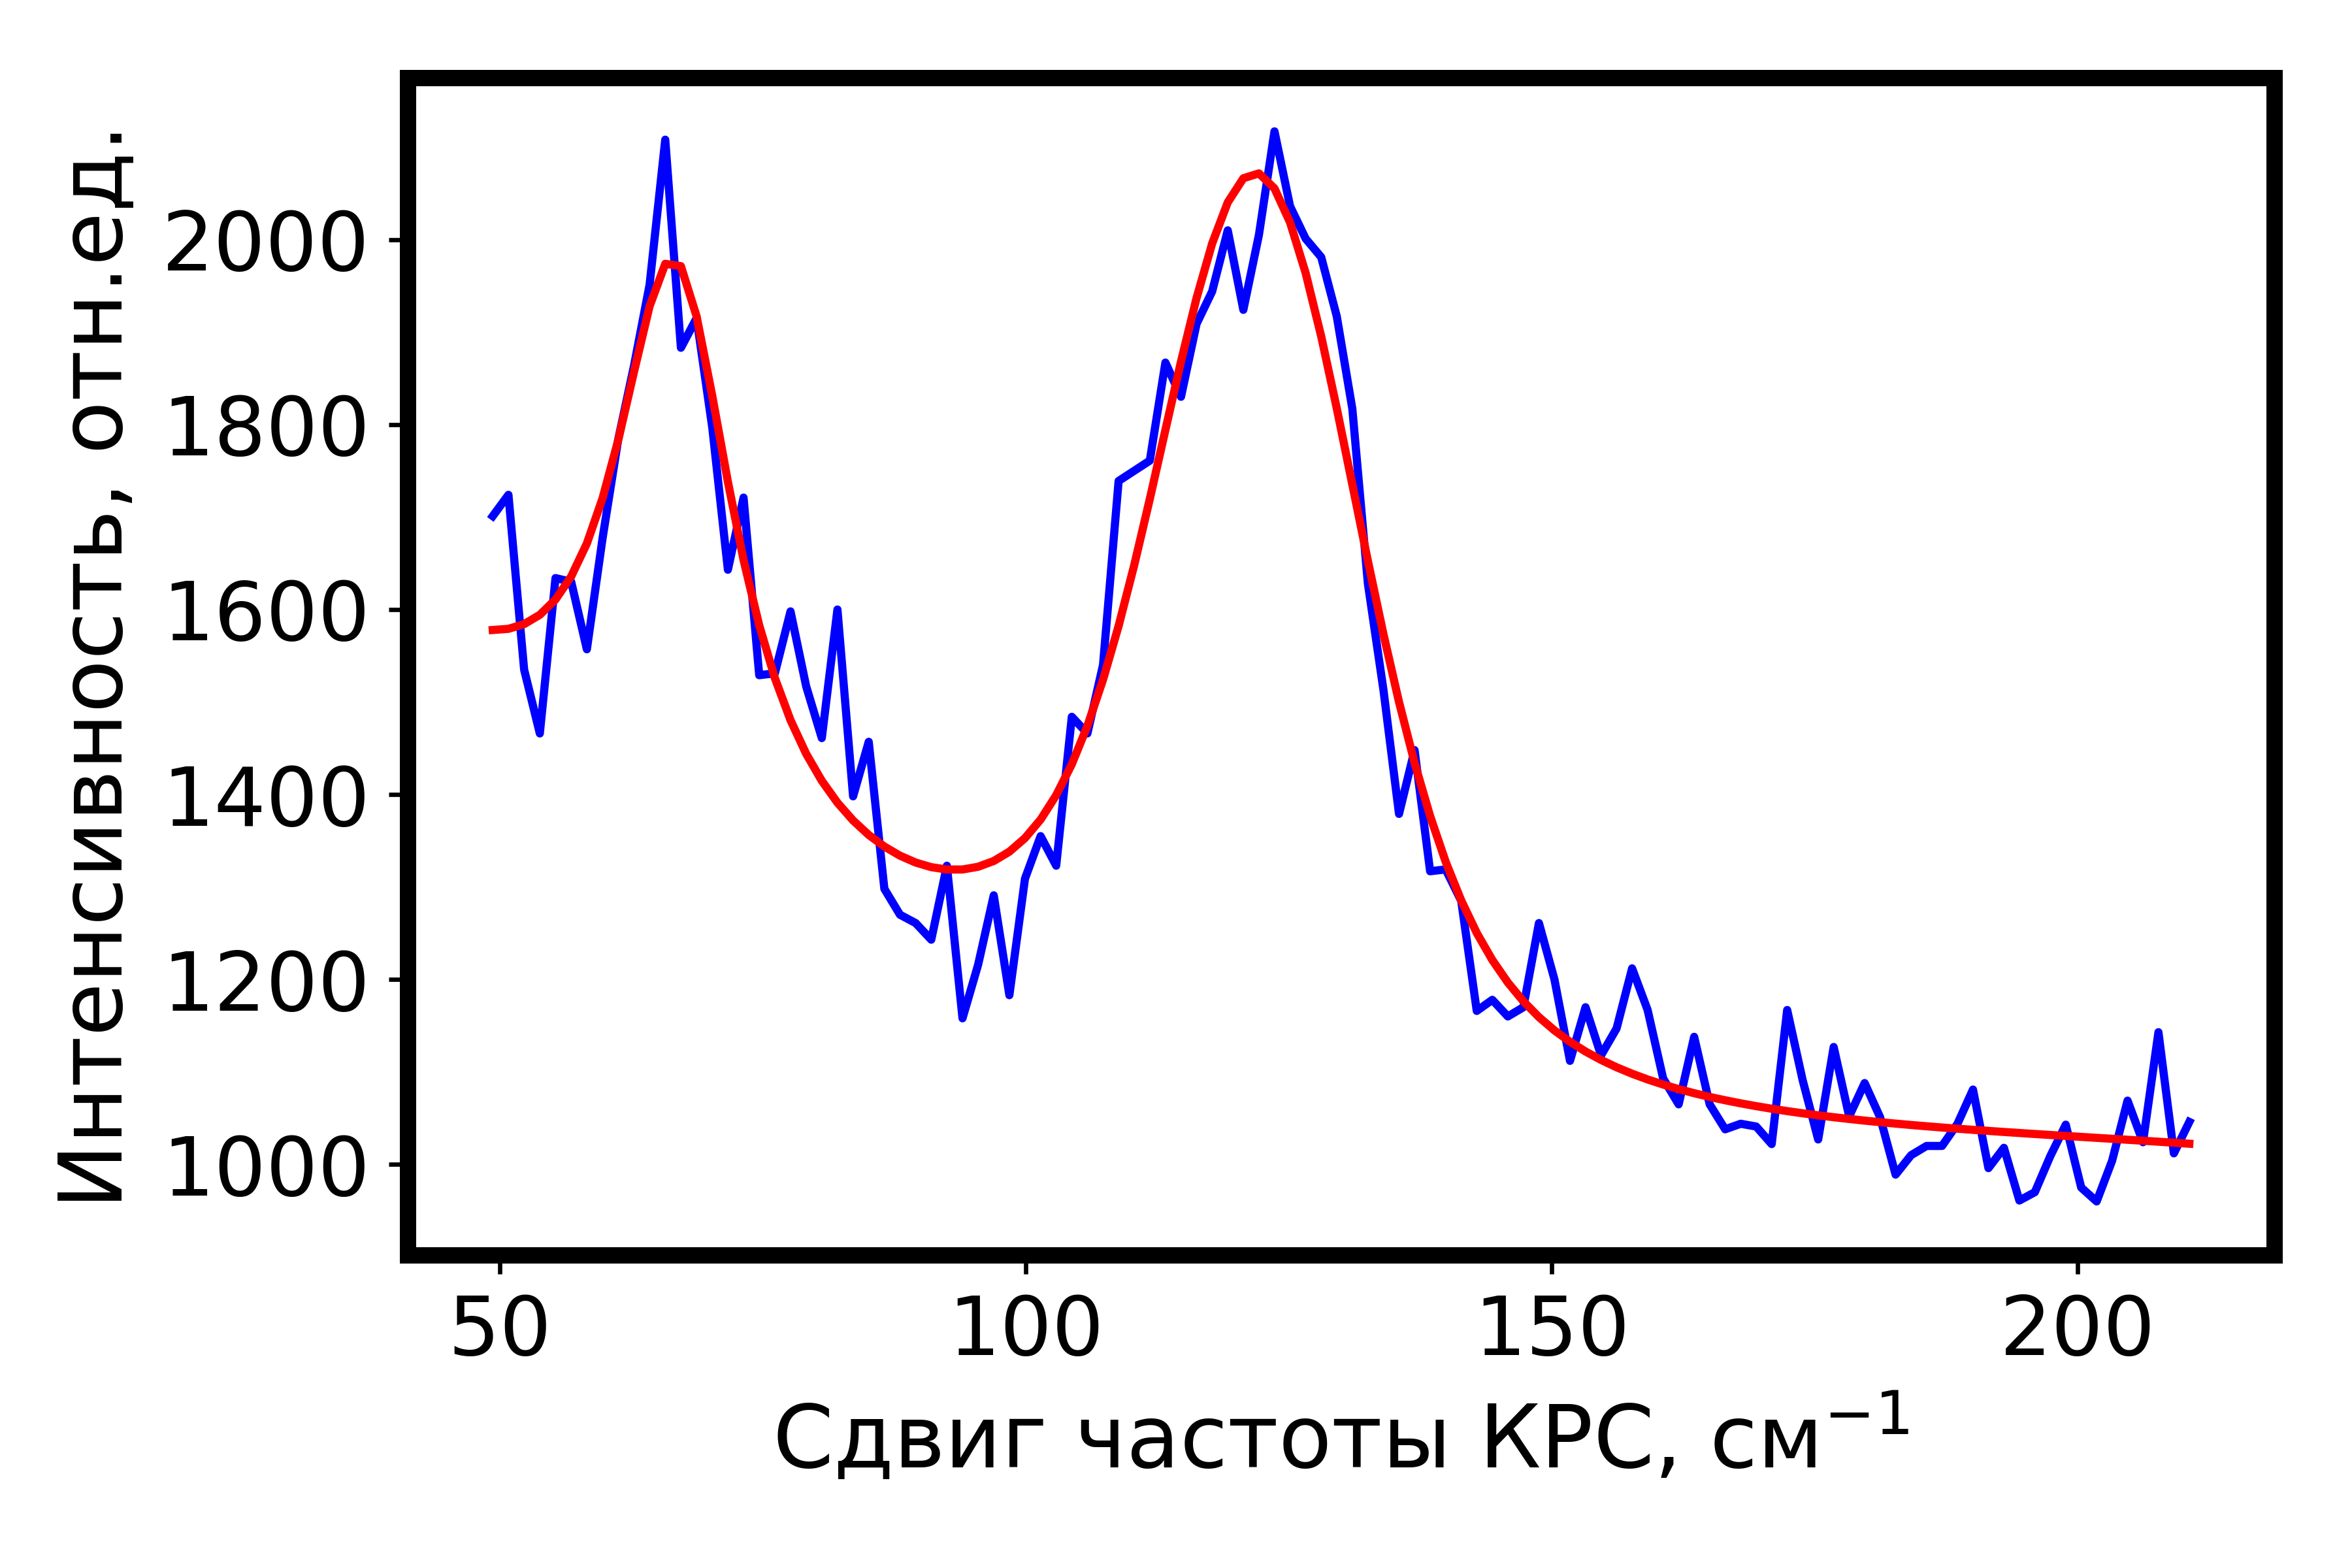
\includegraphics[width=0.9\linewidth]{raman_25_CuAsS3} \\ а)
  \end{minipage}
  \hfill
  \begin{minipage}[ht]{0.5\linewidth}\centering
    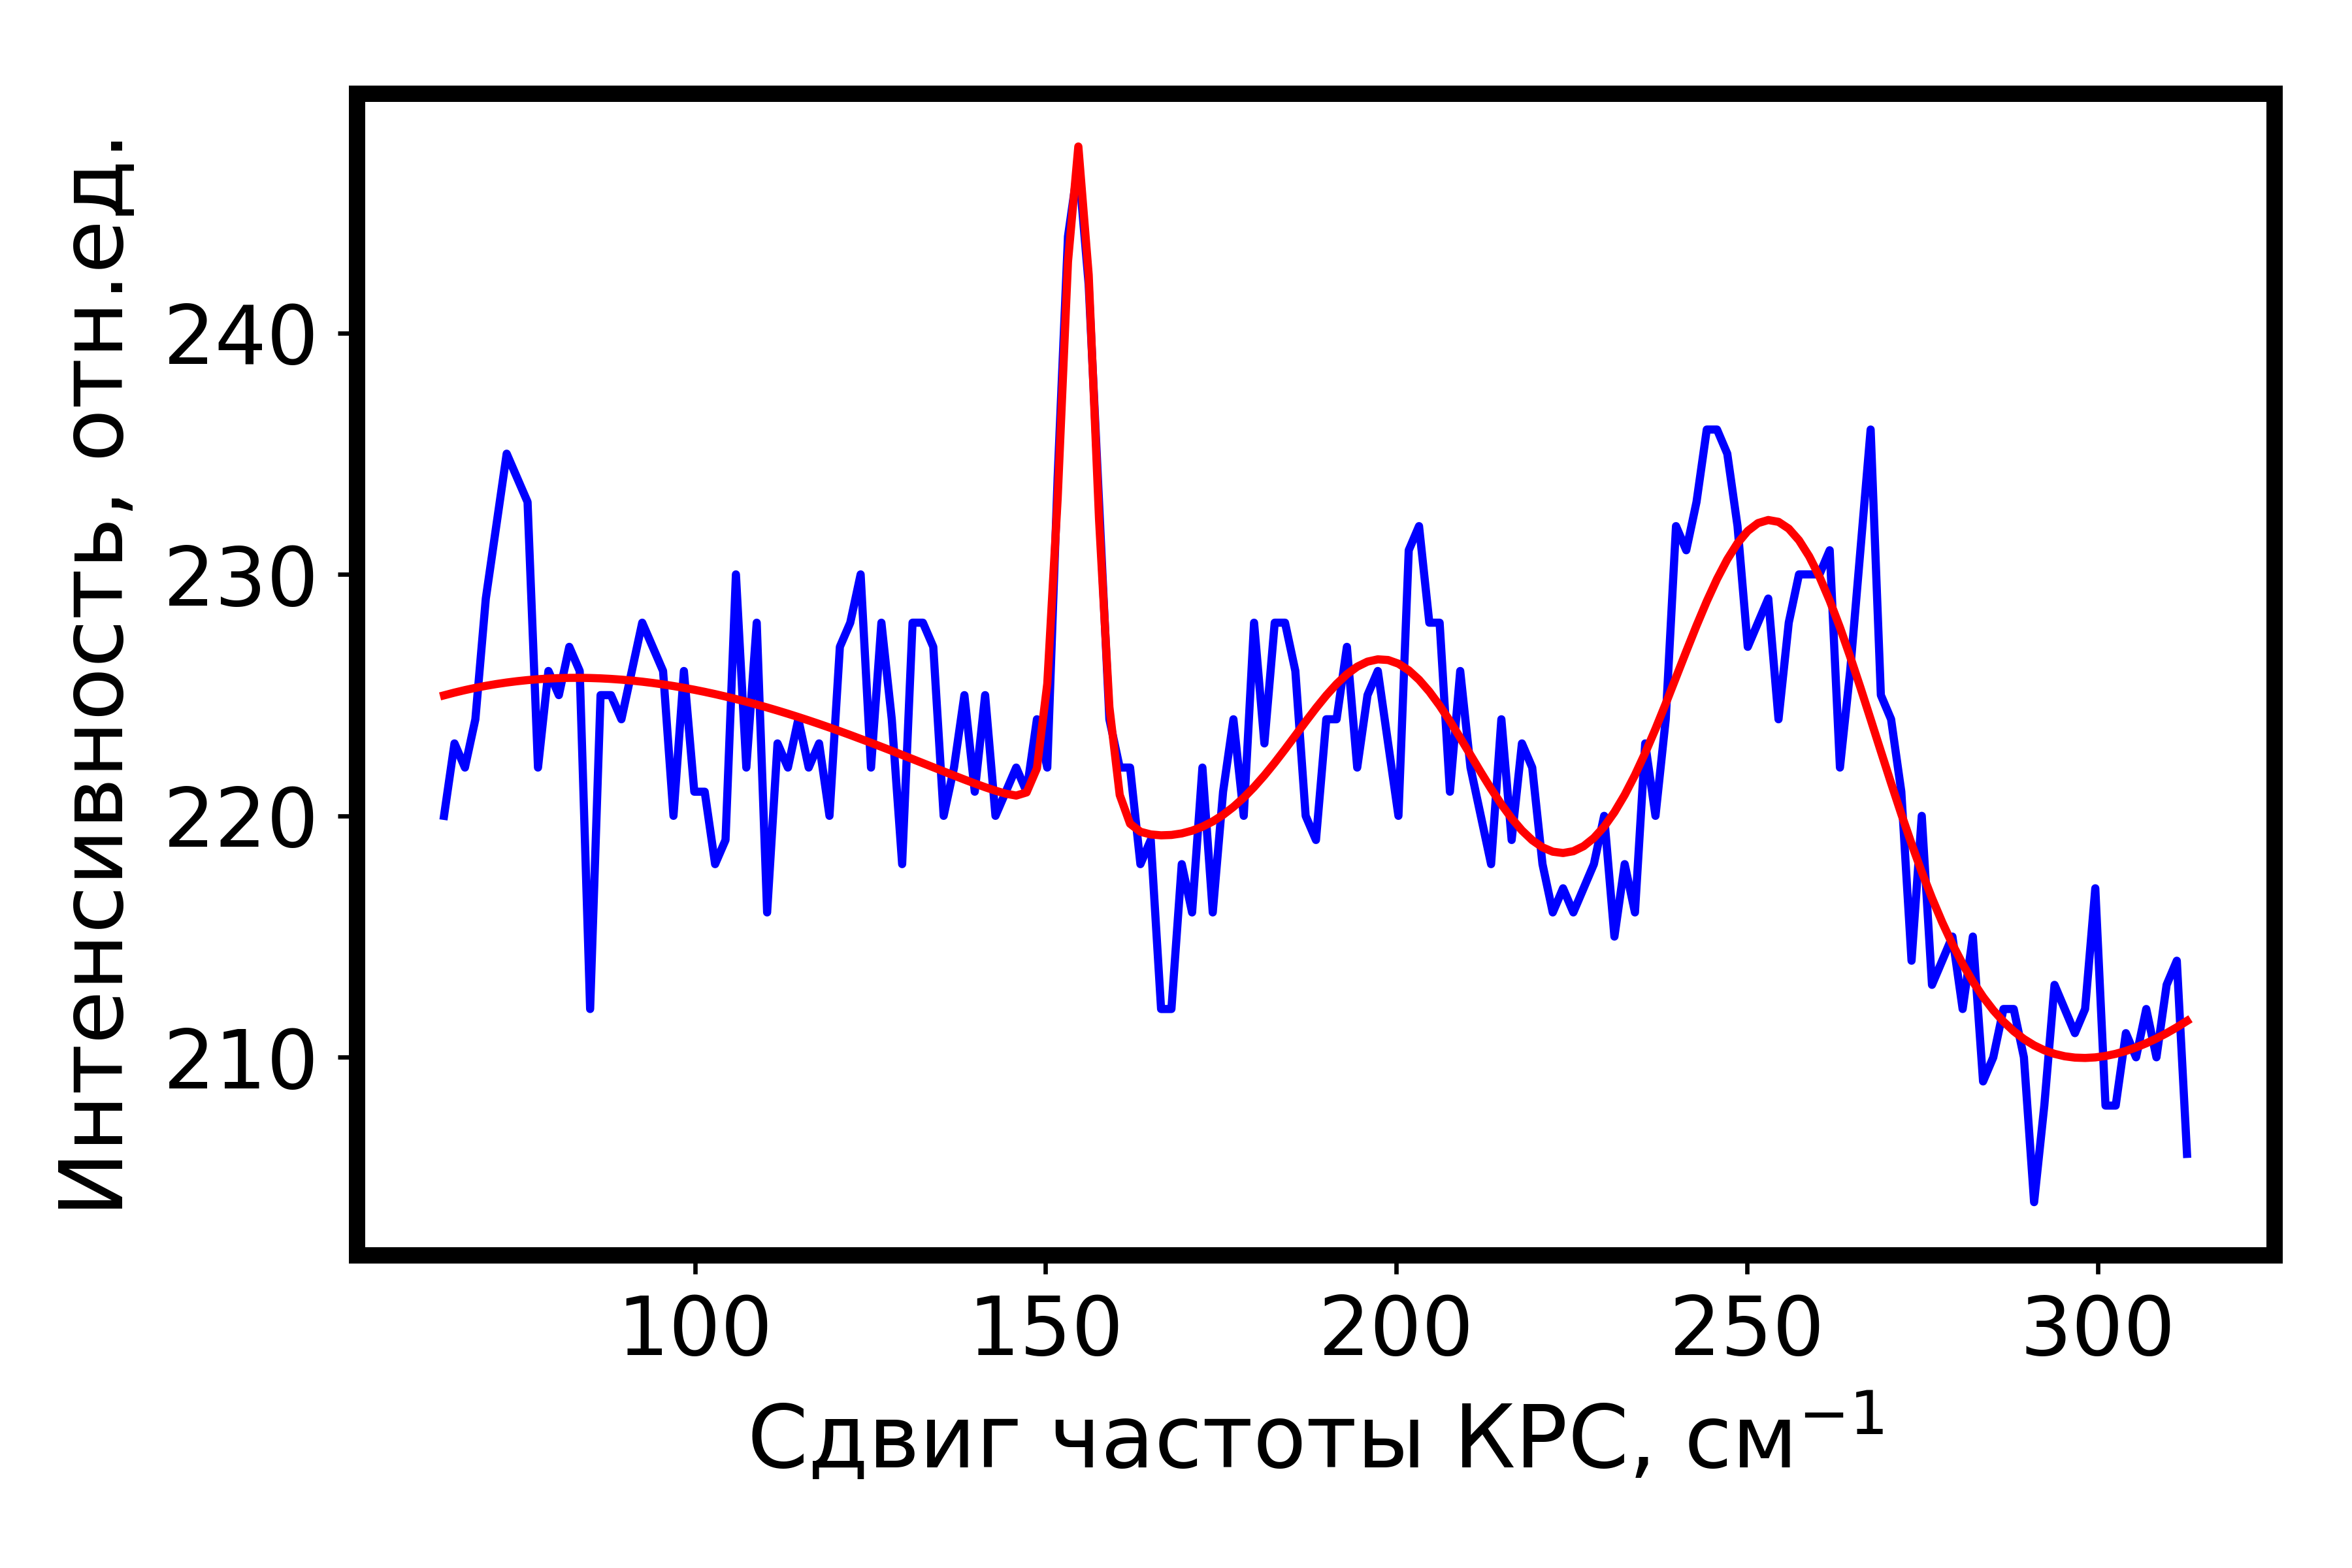
\includegraphics[width=0.9\linewidth]{raman_288_Cu3AsSe3} \\ б)
  \end{minipage}
\vfill
  \begin{minipage}[ht]{0.5\linewidth}\centering
    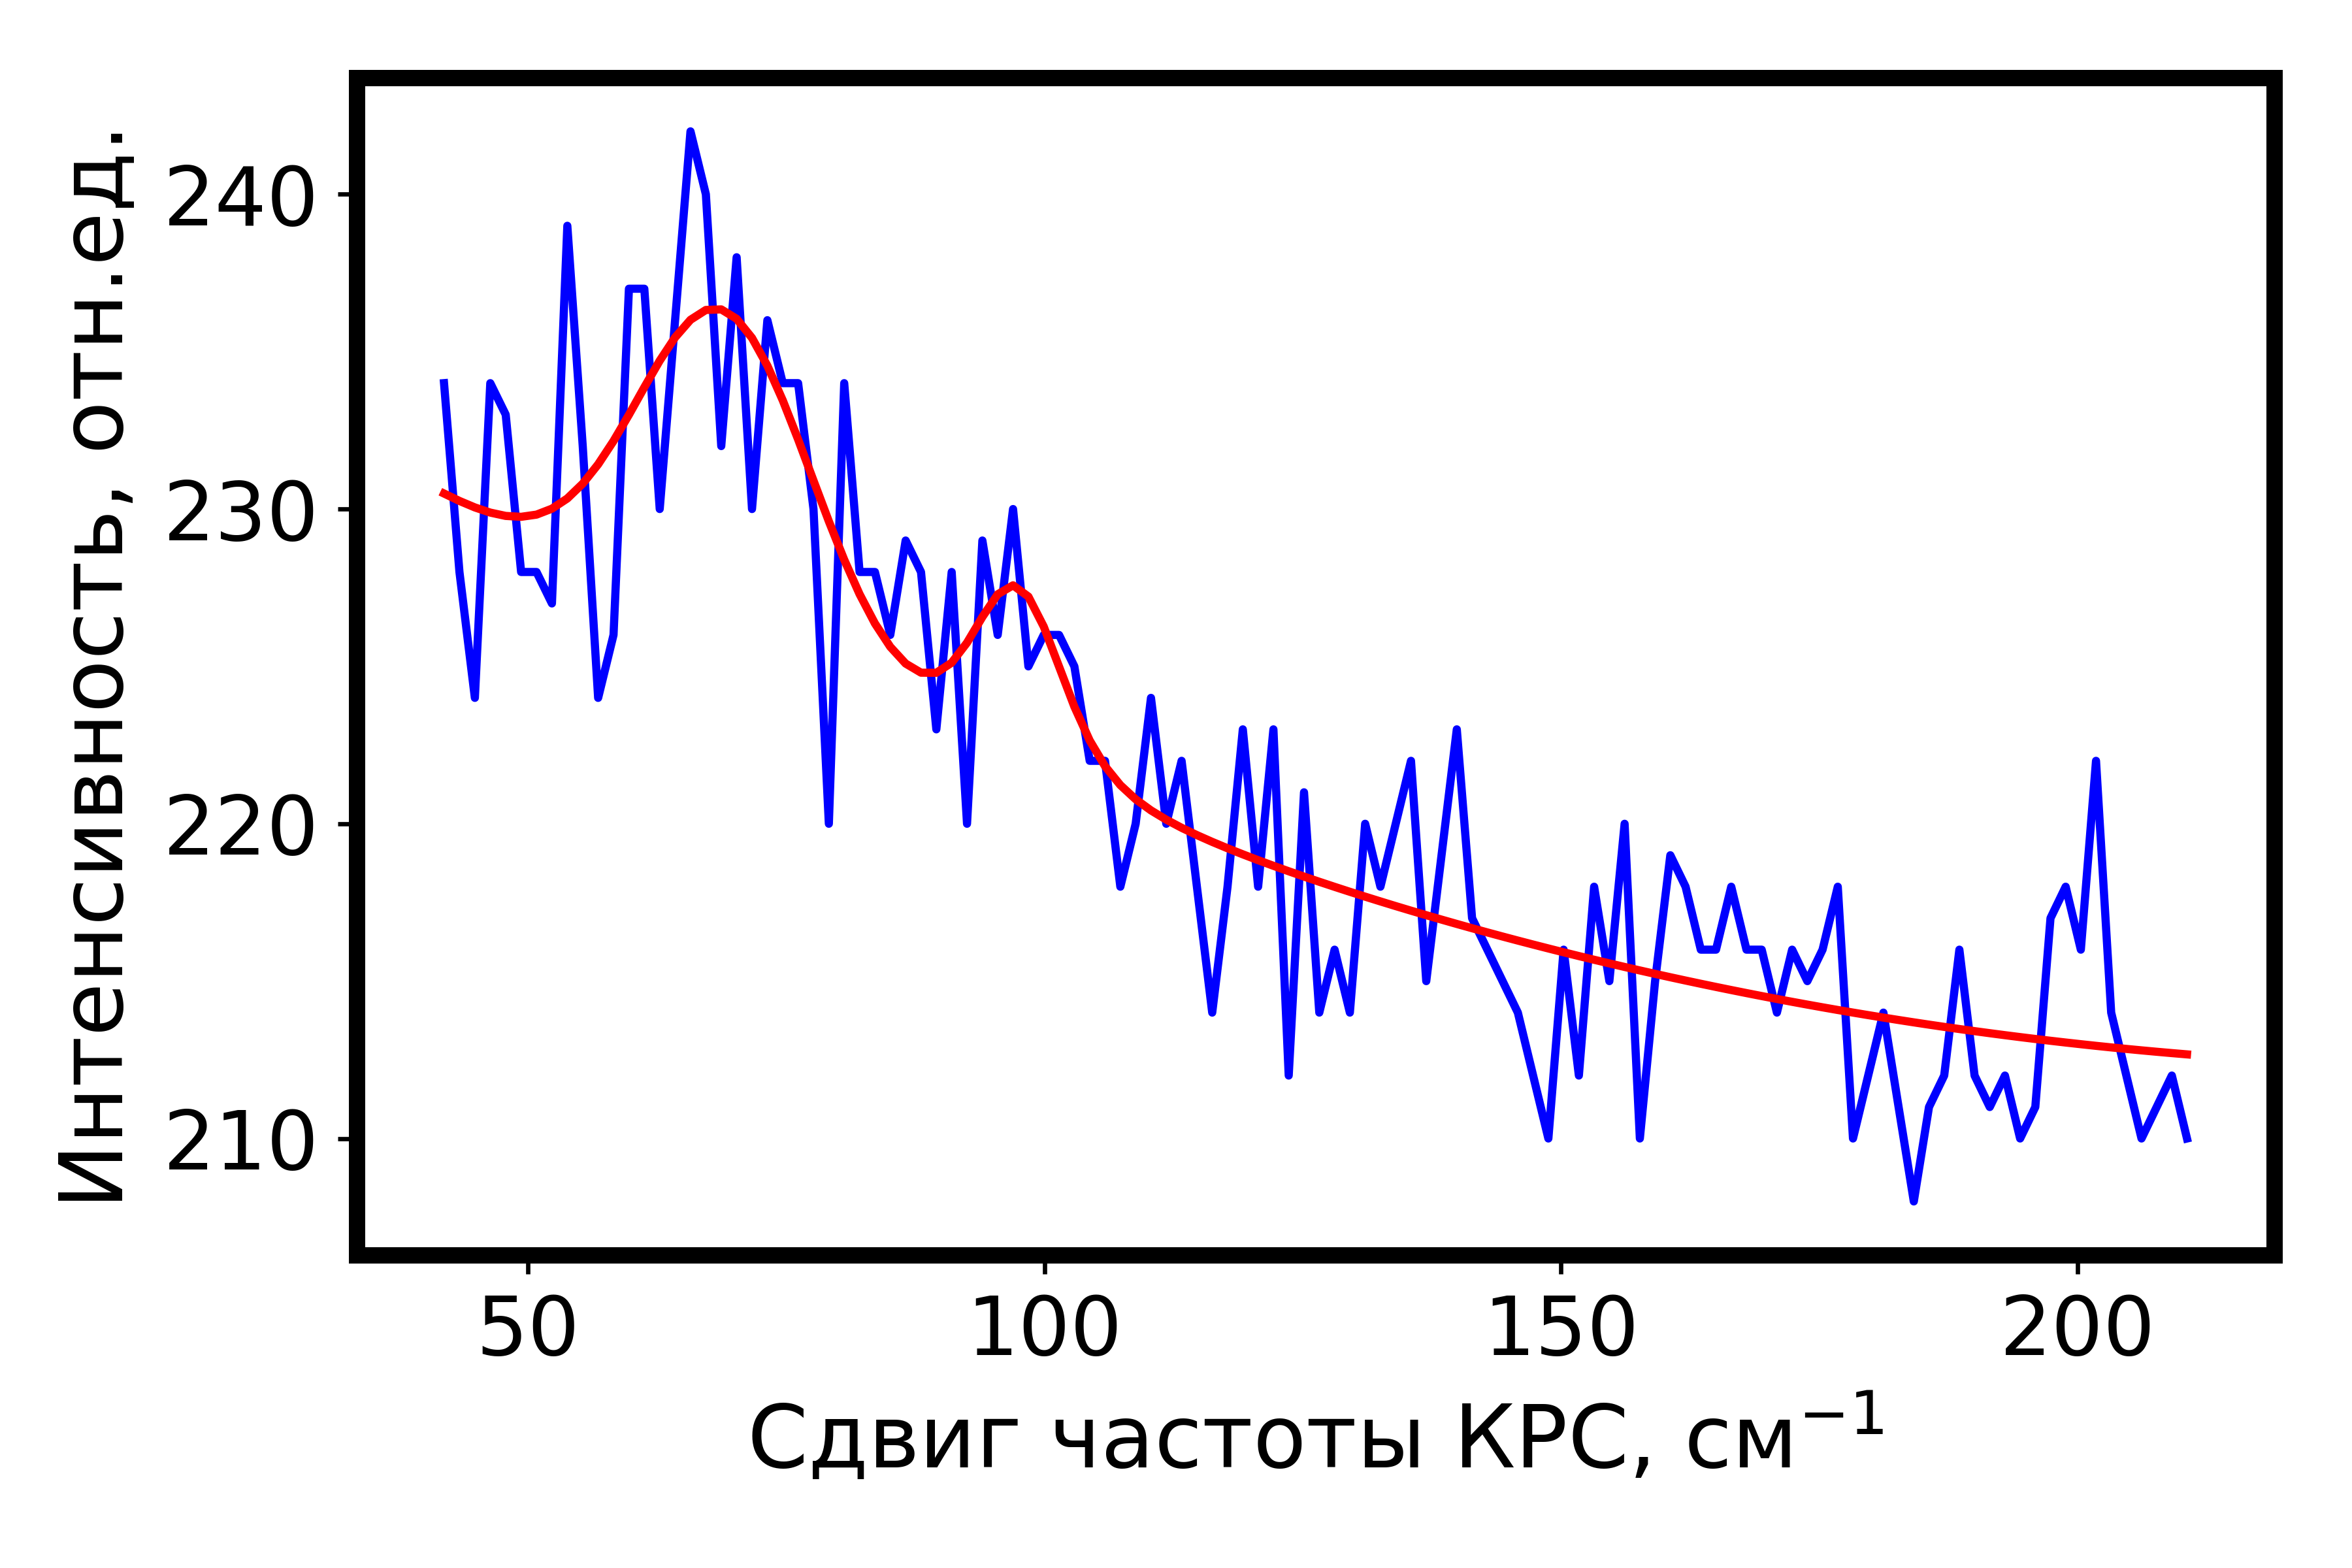
\includegraphics[width=0.9\linewidth]{raman_206_Cu3SbS3} \\ в)
  \end{minipage}
  \hfill
  \begin{minipage}[ht]{0.5\linewidth}\centering
    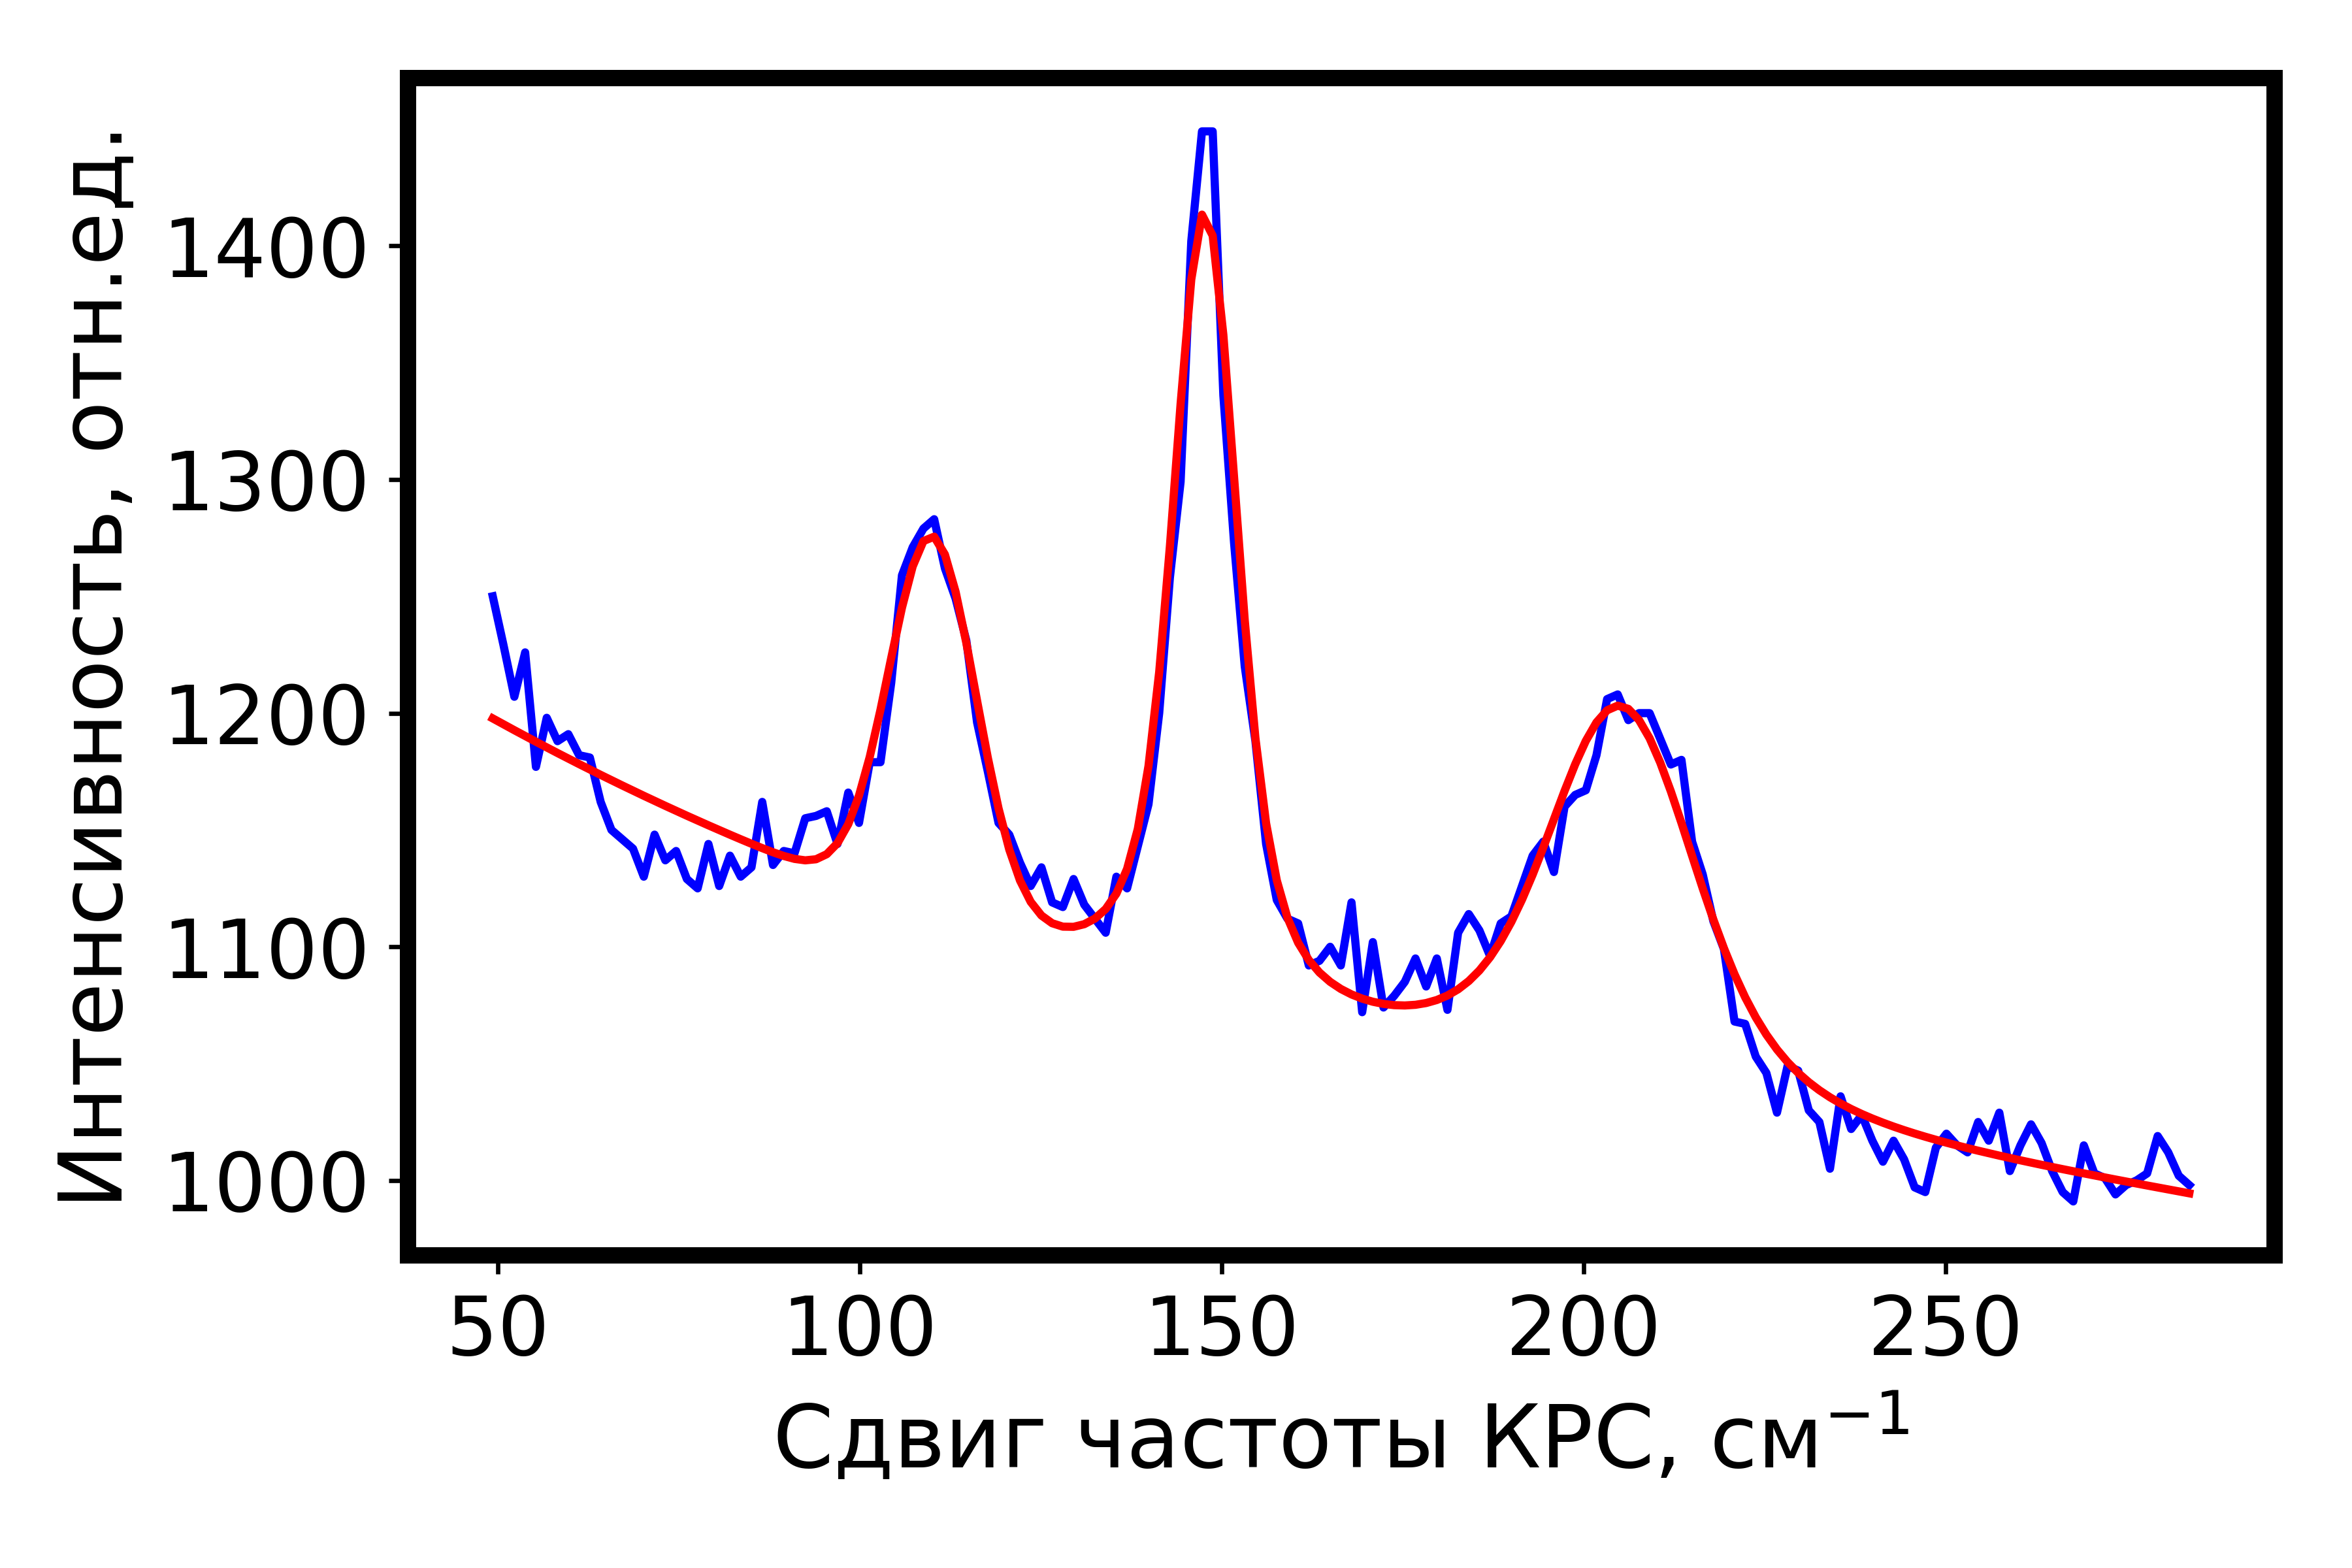
\includegraphics[width=0.9\linewidth]{raman_209_Cu3SbSe3} \\ г)
  \end{minipage}

      \caption[Графики спектров комбинационного рассеяния соединений Cu\textsubscript{12}As\textsubscript{4}S\textsubscript{13} (а), Cu\textsubscript{12}Sb\textsubscript{4}S\textsubscript{13} (б), Cu\textsubscript{3}AsSe\textsubscript{3} (в) и Cu\textsubscript{3}SbSe\textsubscript{3} (г)]{Графики спектров комбинационного рассеяния соединений Cu\textsubscript{12}As\textsubscript{4}S\textsubscript{13} (а), Cu\textsubscript{12}Sb\textsubscript{4}S\textsubscript{13} (б), Cu\textsubscript{3}AsSe\textsubscript{3} (в) и Cu\textsubscript{3}SbSe\textsubscript{3} (г)}
    \label{img:figure_raman}
\end{figure}


\begin{figure}[b!]
  \begin{minipage}[ht]{0.5\linewidth}\centering
    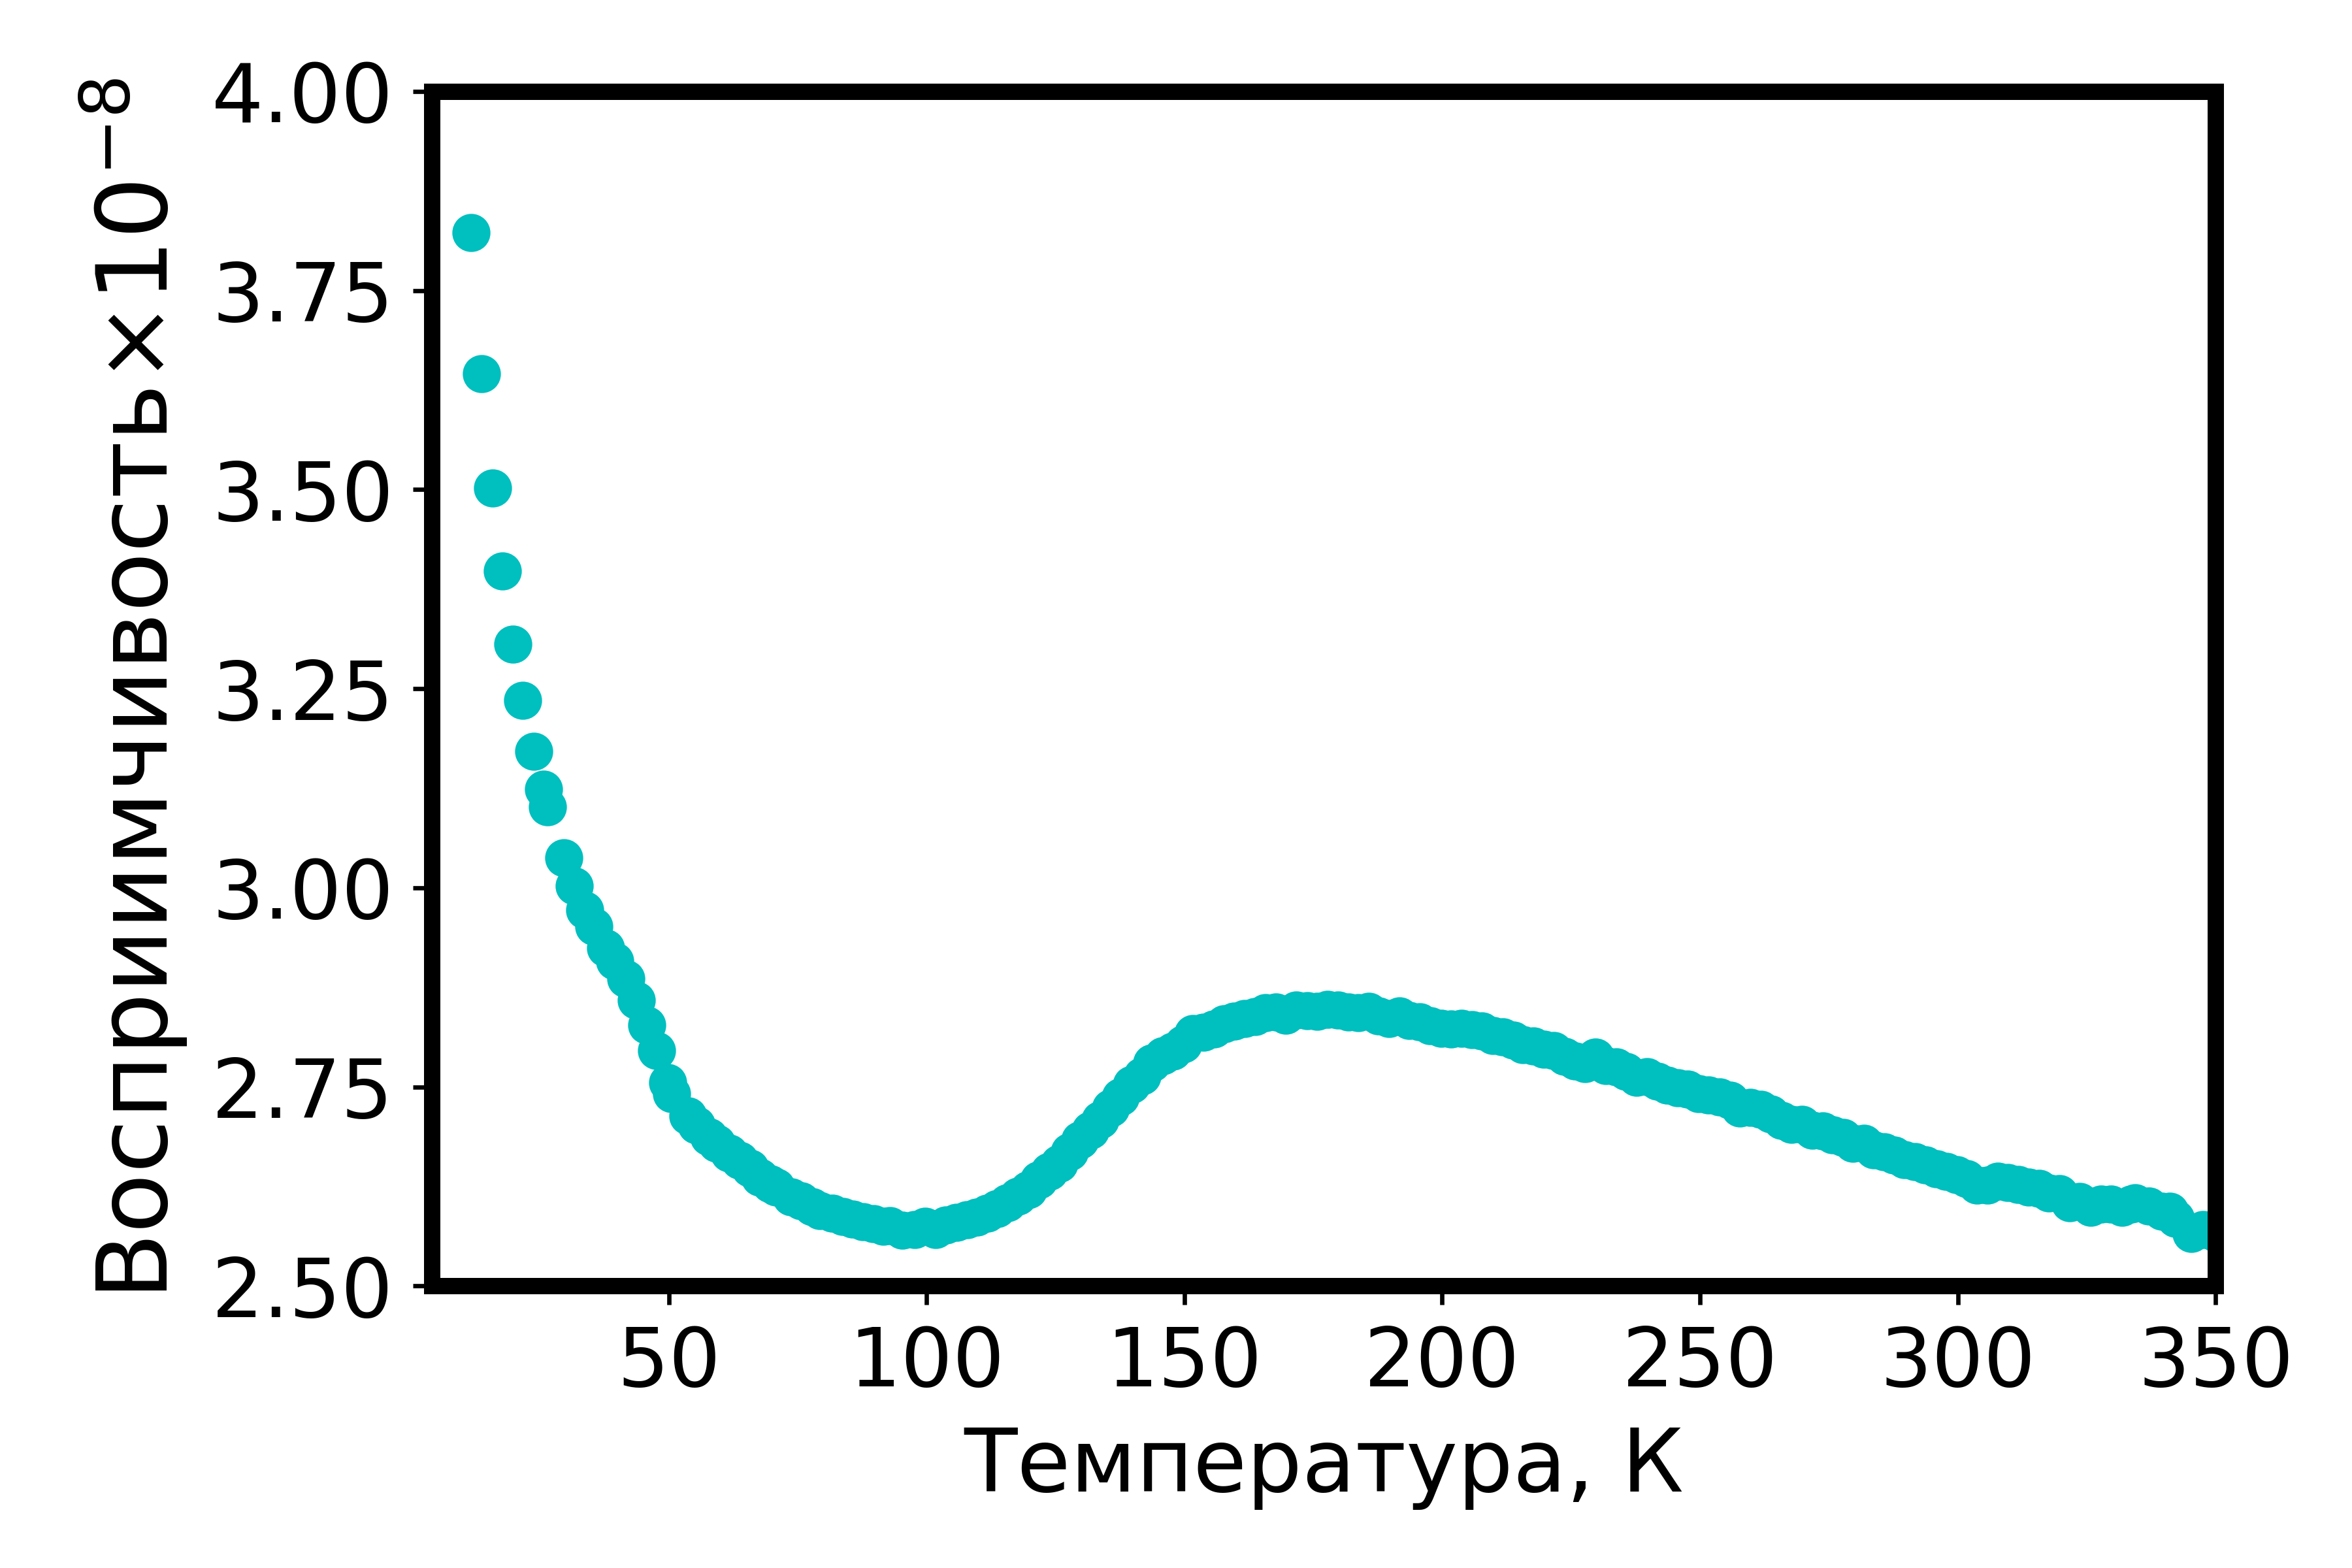
\includegraphics[width=0.9\linewidth]{sus_exp_Cu_As_S} \\ а)
  \end{minipage}
  \hfill
  \begin{minipage}[ht]{0.5\linewidth}\centering
    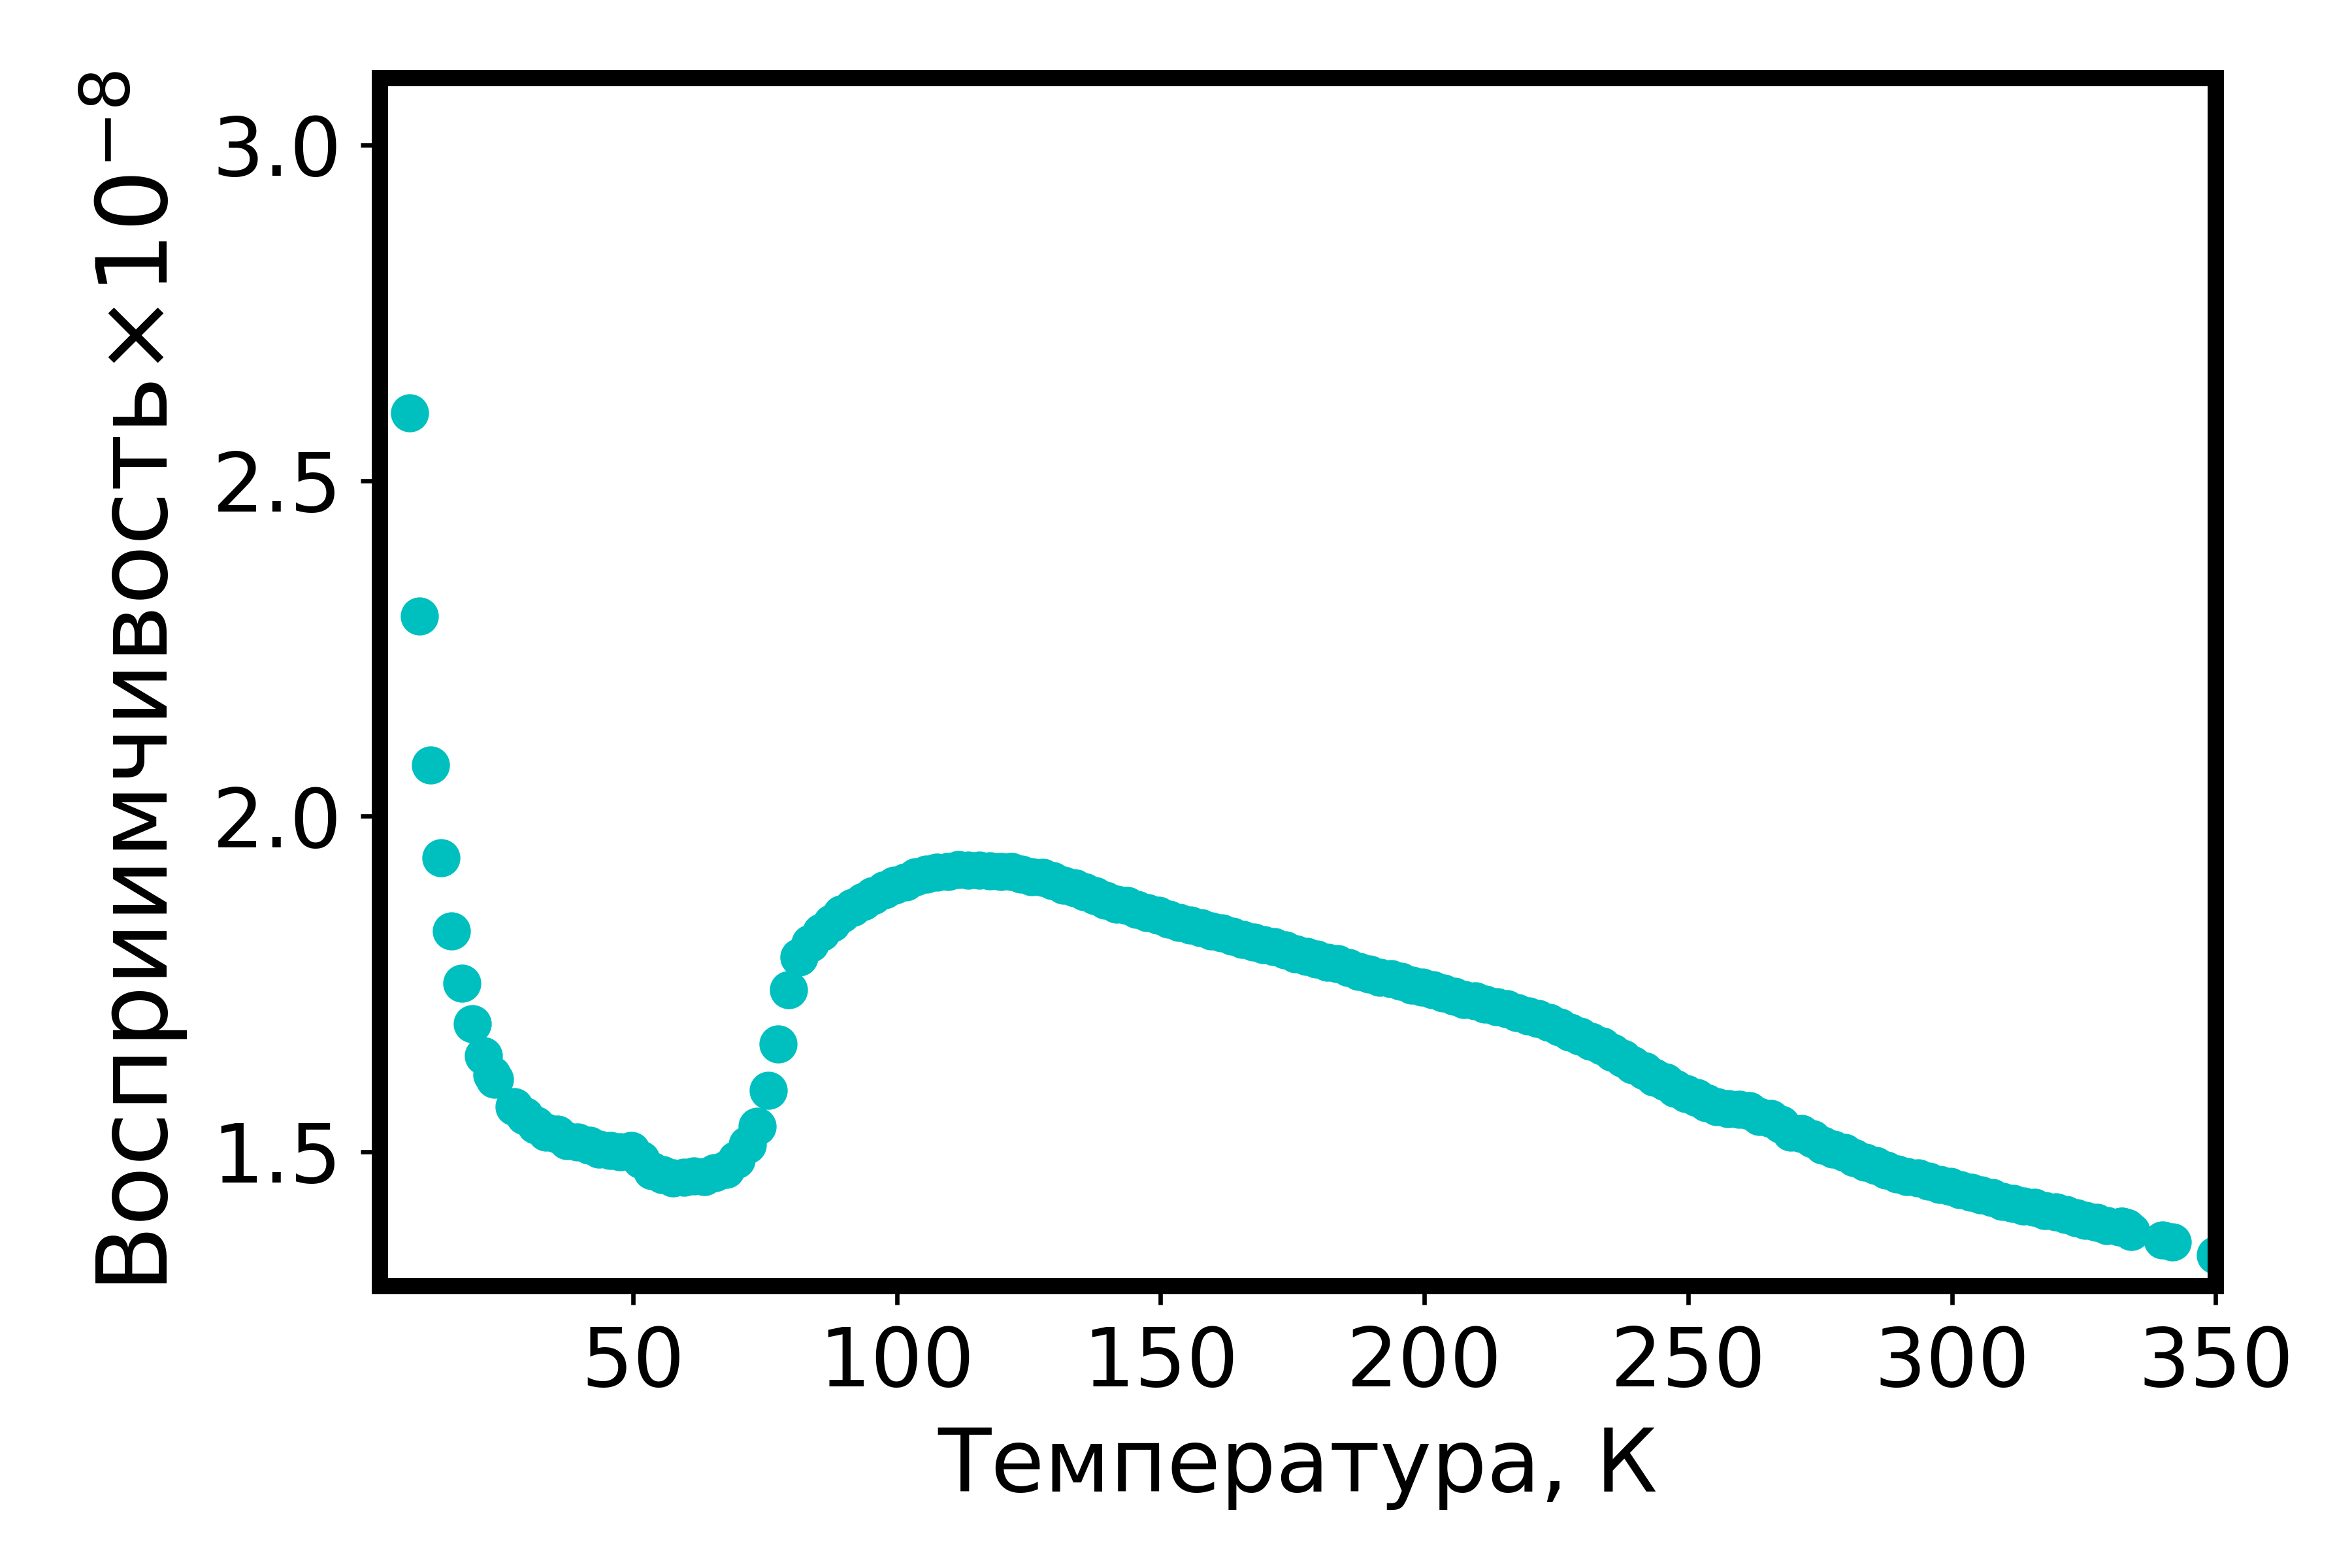
\includegraphics[width=0.9\linewidth]{sus_exp_Cu_Sb_S} \\ б)
  \end{minipage}
\vfill
  \begin{minipage}[ht]{0.5\linewidth}\centering
    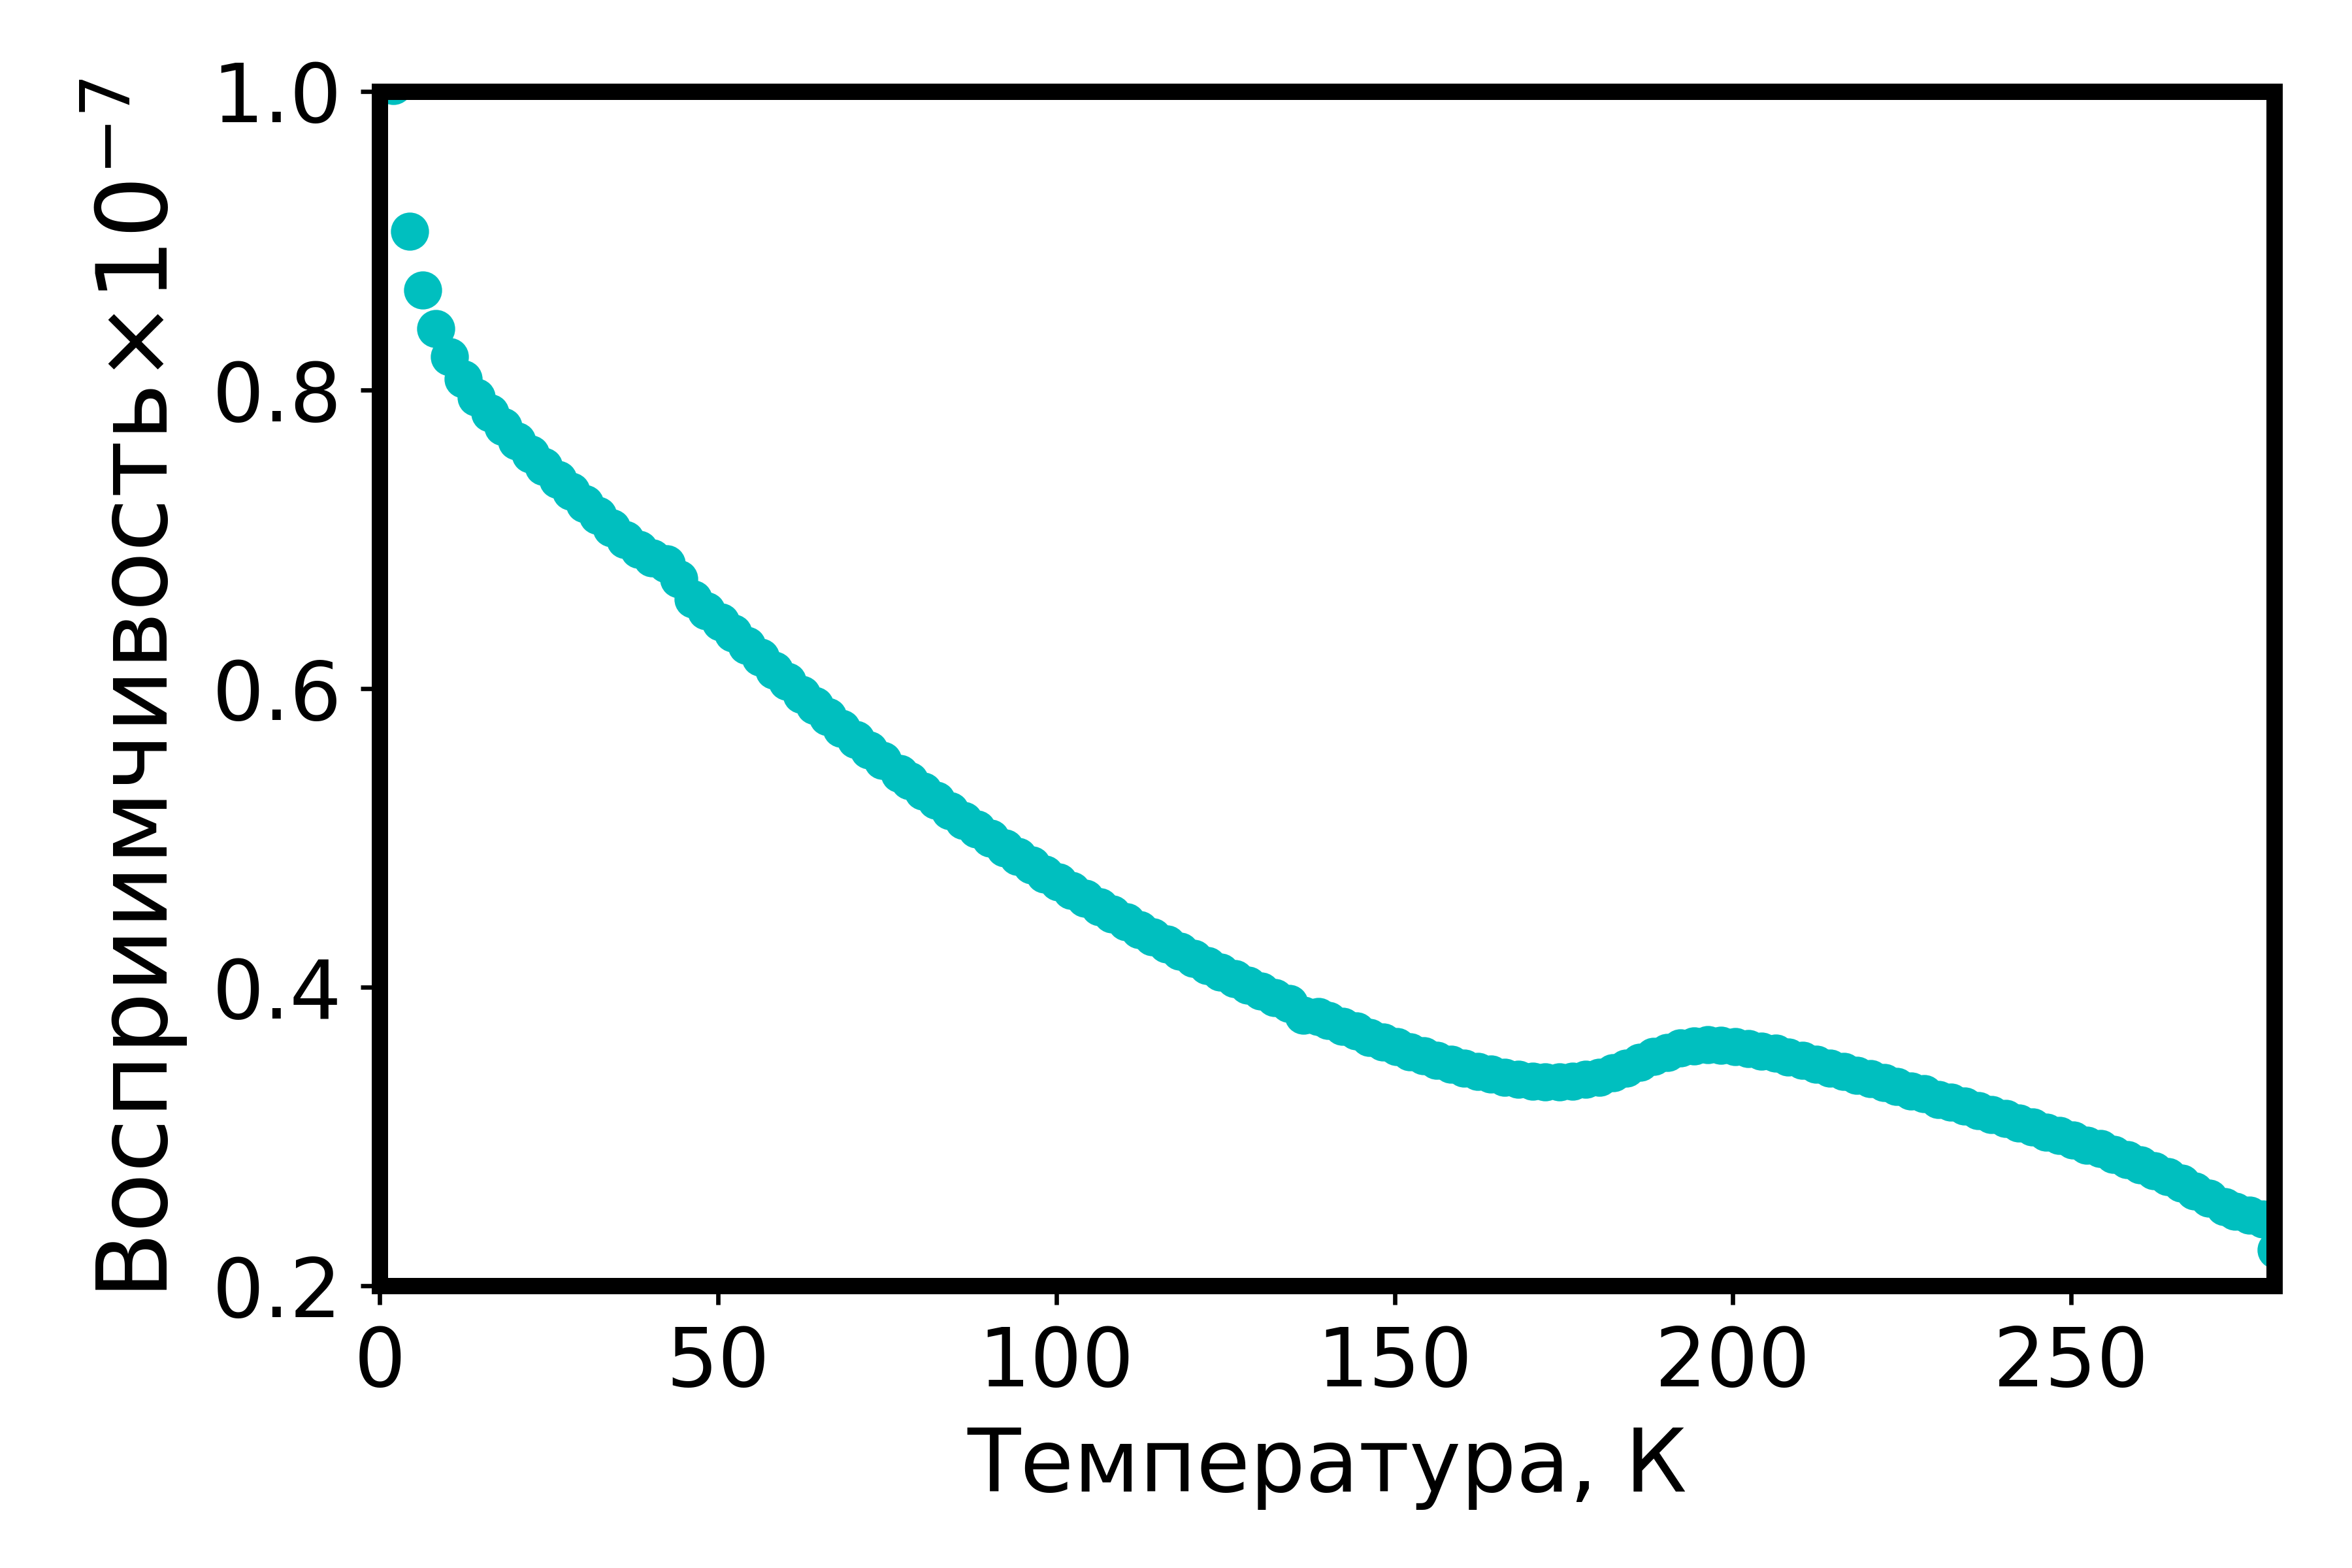
\includegraphics[width=0.9\linewidth]{sus_exp_Cu_As_Se} \\ в)
  \end{minipage}
  \hfill
  \begin{minipage}[ht]{0.5\linewidth}\centering
    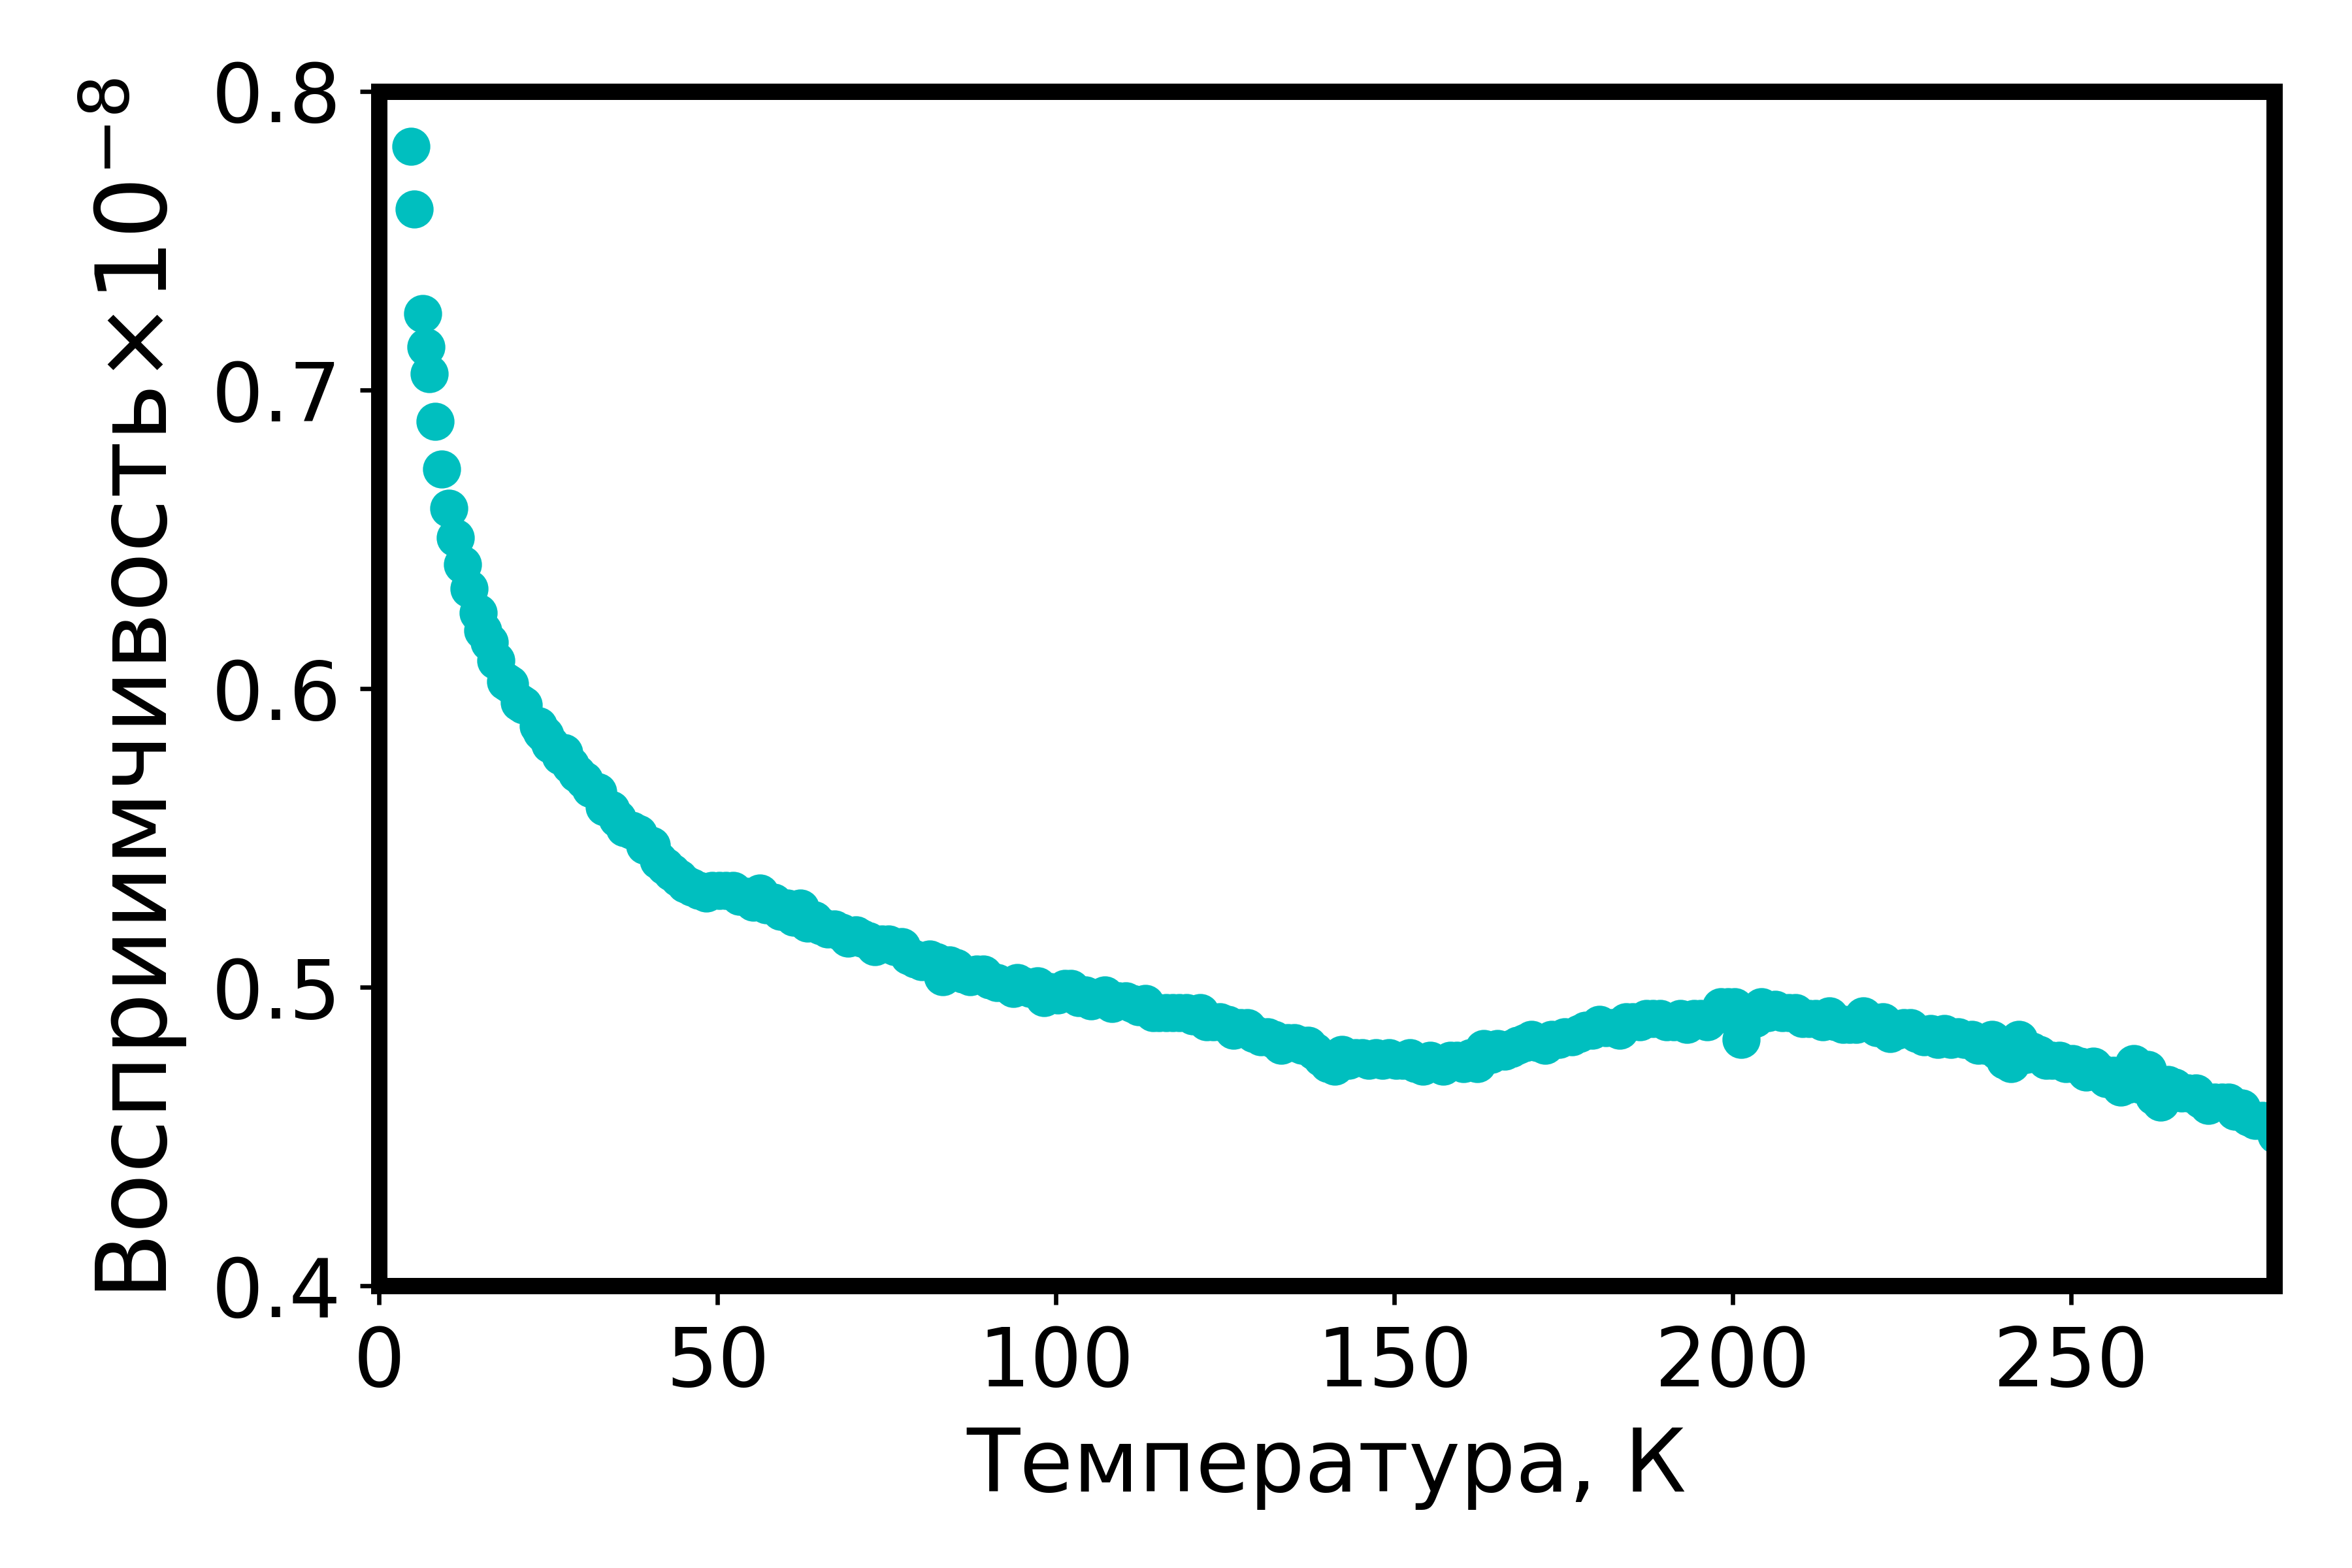
\includegraphics[width=0.9\linewidth]{sus_exp_Cu_Sb_Se} \\ г)
  \end{minipage}

      \caption[Графики температурных зависимостей магнитной восприимчивости для соединений Cu\textsubscript{12}As\textsubscript{4}S\textsubscript{13} (а), Cu\textsubscript{12}Sb\textsubscript{4}S\textsubscript{13} (б), Cu\textsubscript{3}AsSe\textsubscript{3} (в) и Cu\textsubscript{3}SbSe\textsubscript{3} (г)]{Графики температурных зависимостей магнитной восприимчивости для соединений Cu\textsubscript{12}As\textsubscript{4}S\textsubscript{13} (а), Cu\textsubscript{12}Sb\textsubscript{4}S\textsubscript{13} (б), Cu\textsubscript{3}AsSe\textsubscript{3} (в) и Cu\textsubscript{3}SbSe\textsubscript{3} (г)}
    \label{img:figure3}
\end{figure}

Температурные зависимости магнитной восприимчивости для каждого
 образца были получены в магнитных полях 1, 10, 35 и 70 кЭ (Рис. \ref{img:figure3}).
При любом значении магнитного поля графики зависимости магнитной восприимчивости
 имеют одинаковые характерные особенности для всех исследованных соединений.
 Также зависимости магнитной восприимчивости для монокристаллического и
 поликристаллических образцов соединения Cu\textsubscript{12}As\textsubscript{4}S\textsubscript{13} не отличаются.
Все зависимости магнитной восприимчивости приведены с вычетом диамагнитного вклада.
%Полученные зависимости обладают формой, характерной для парамагнетиков с существенными отклонениями от парамагнитного хода.
На графиках температурных зависимостей магнитной восприимчивости для соединений Cu\textsubscript{12}As\textsubscript{4}S\textsubscript{13} и Cu\textsubscript{12}Sb\textsubscript{4}S\textsubscript{13}  наблюдаются отклонения от монотонного парамагнитного хода при температурах T$\approx$124 К и T$\approx$84 К соответственно, и для Cu\textsubscript{3}AsSe\textsubscript{3} и Cu\textsubscript{3}SbSe\textsubscript{3}~"---  T$\approx$170"--~270 К и T$\approx$170"--~300~К соответственно.






%На рисунке~\ref{img:xray} представлены величина заселенности позиций атома Cu2 и изменение значения коэфициента атомарного смещения для позиции атома S2 в диапазоне температур от 85 до 293~К. Аномальное изменение значения коэфициента атомарного смещения для позиции атома S2 показывает наличие фазового перехода второго рода в диапазоне от 115 до 180 К.

%\begin{figure}[ht]
%  \begin{minipage}[ht]{0.5\linewidth}\centering
%    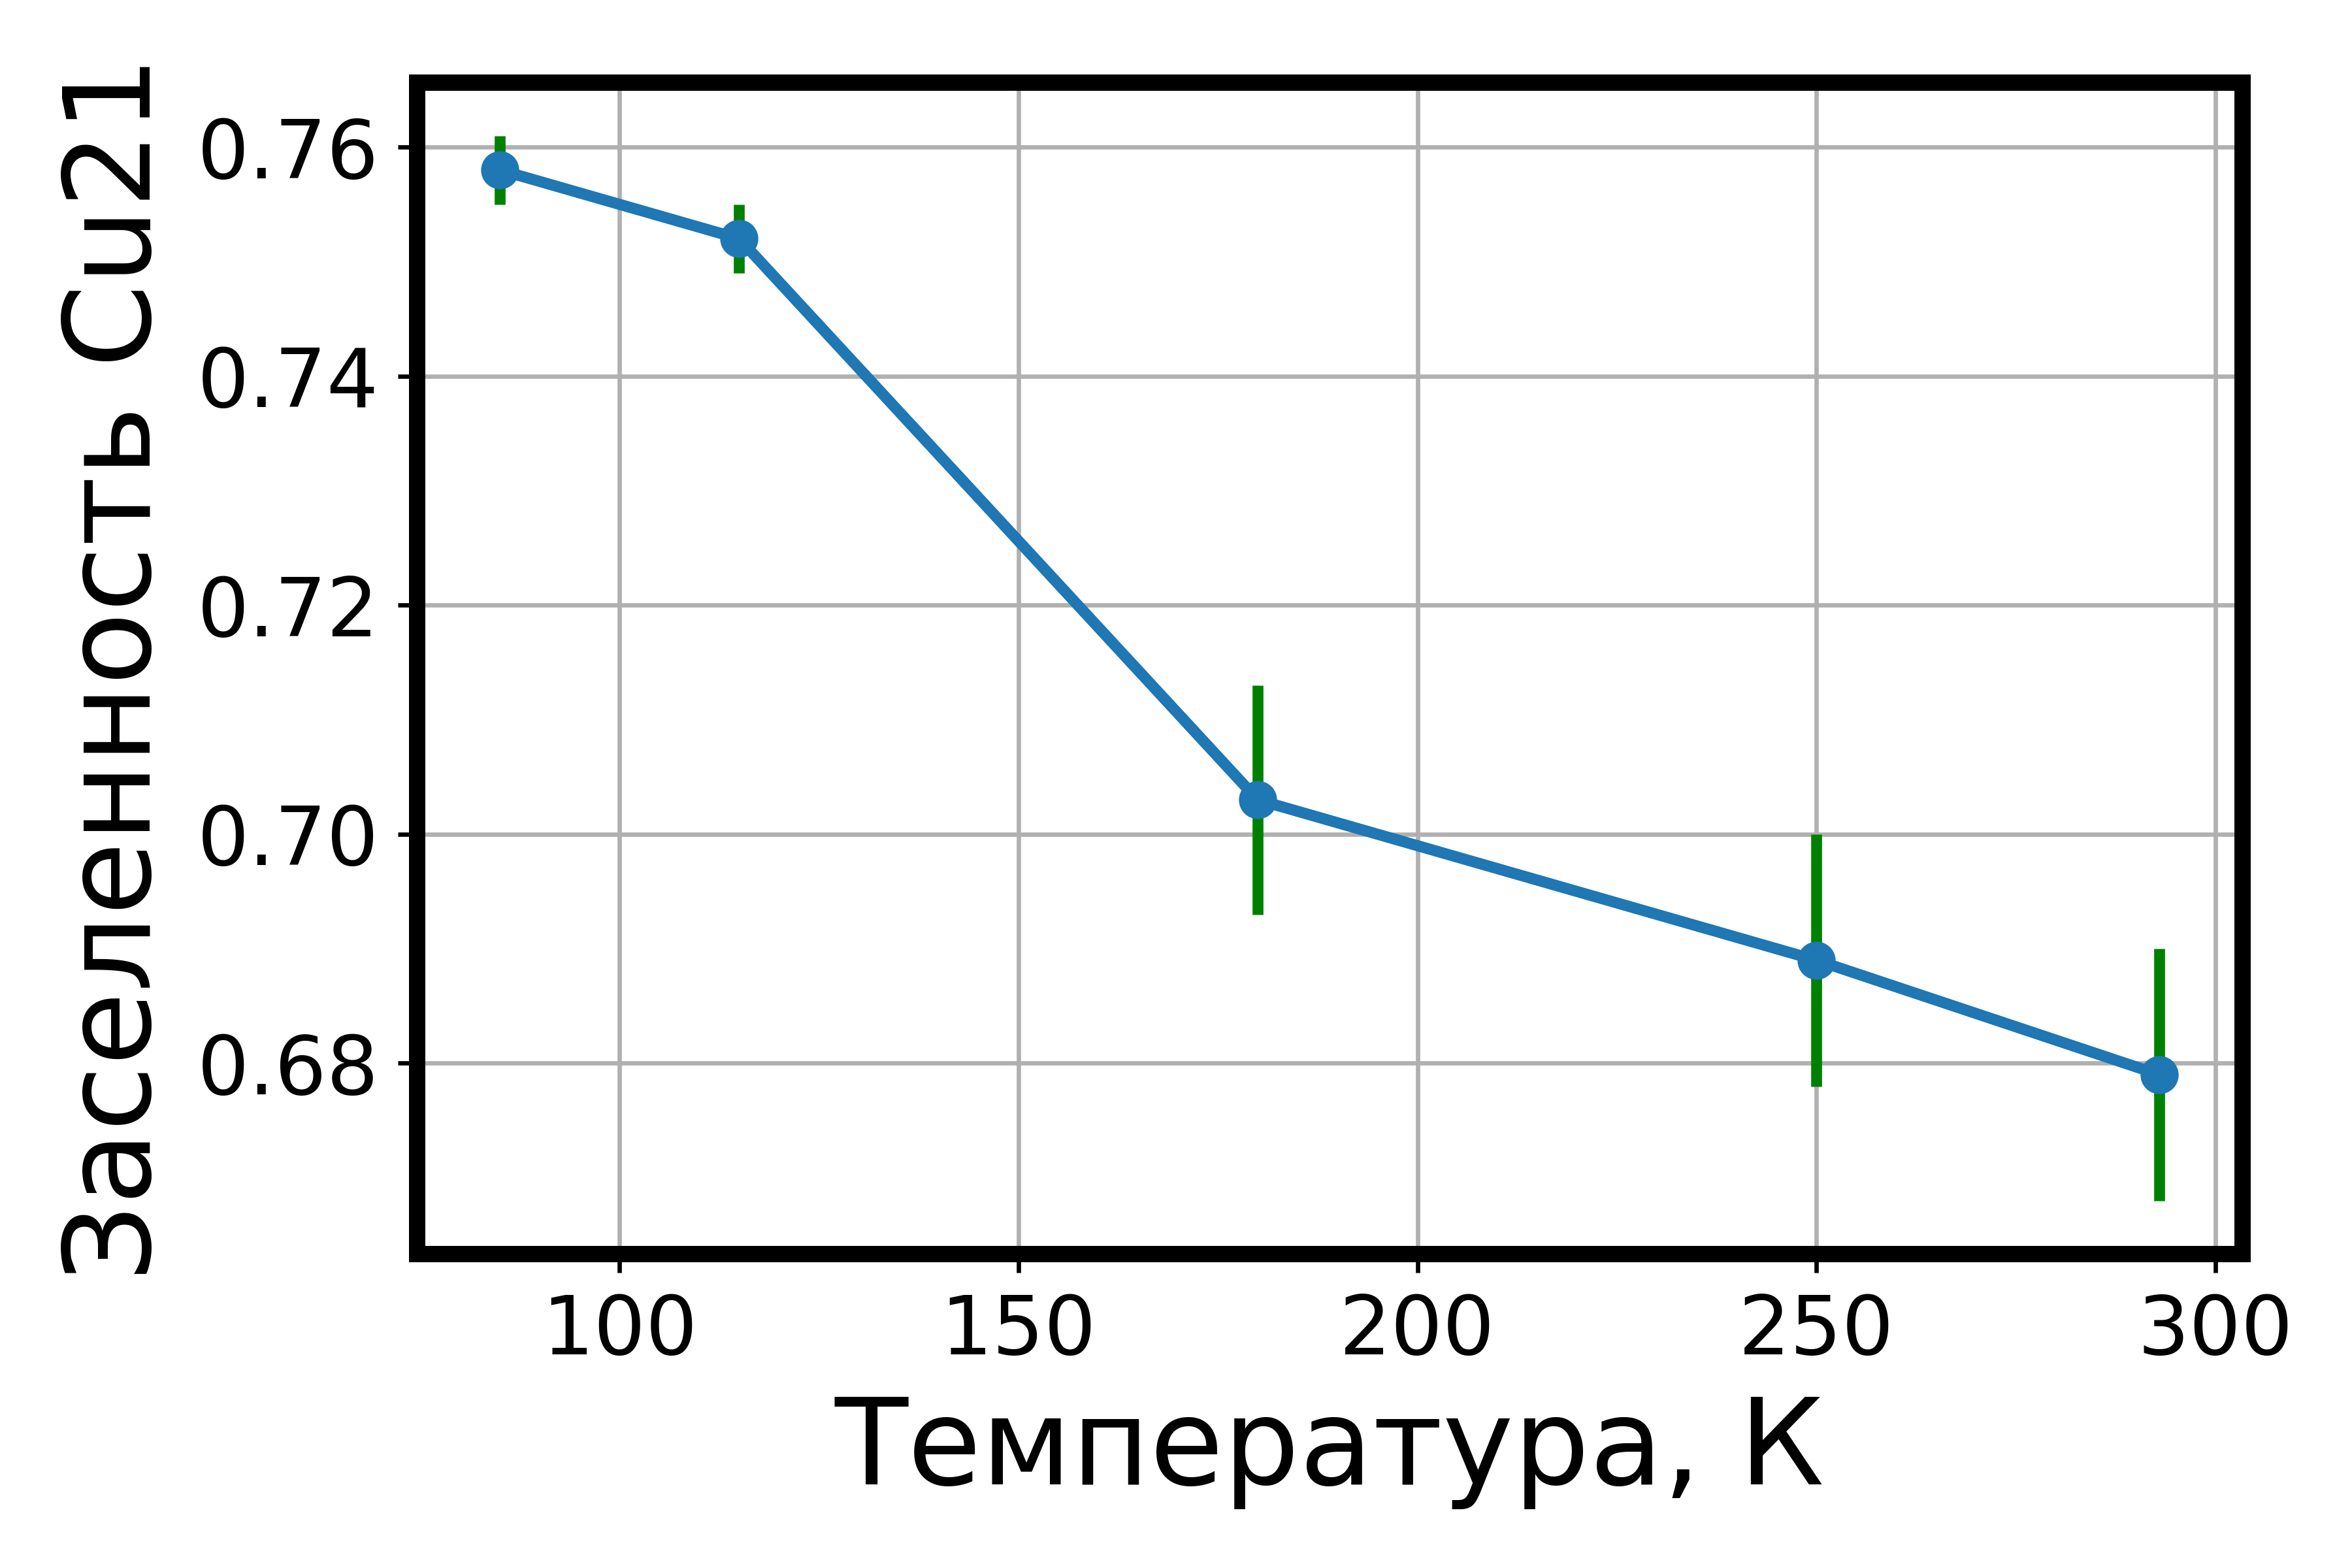
\includegraphics[width=0.9\linewidth]{structure_occCu2} \\ а)
%  \end{minipage}
 % \hfill
 % \begin{minipage}[ht]{0.5\linewidth}\centering
 %   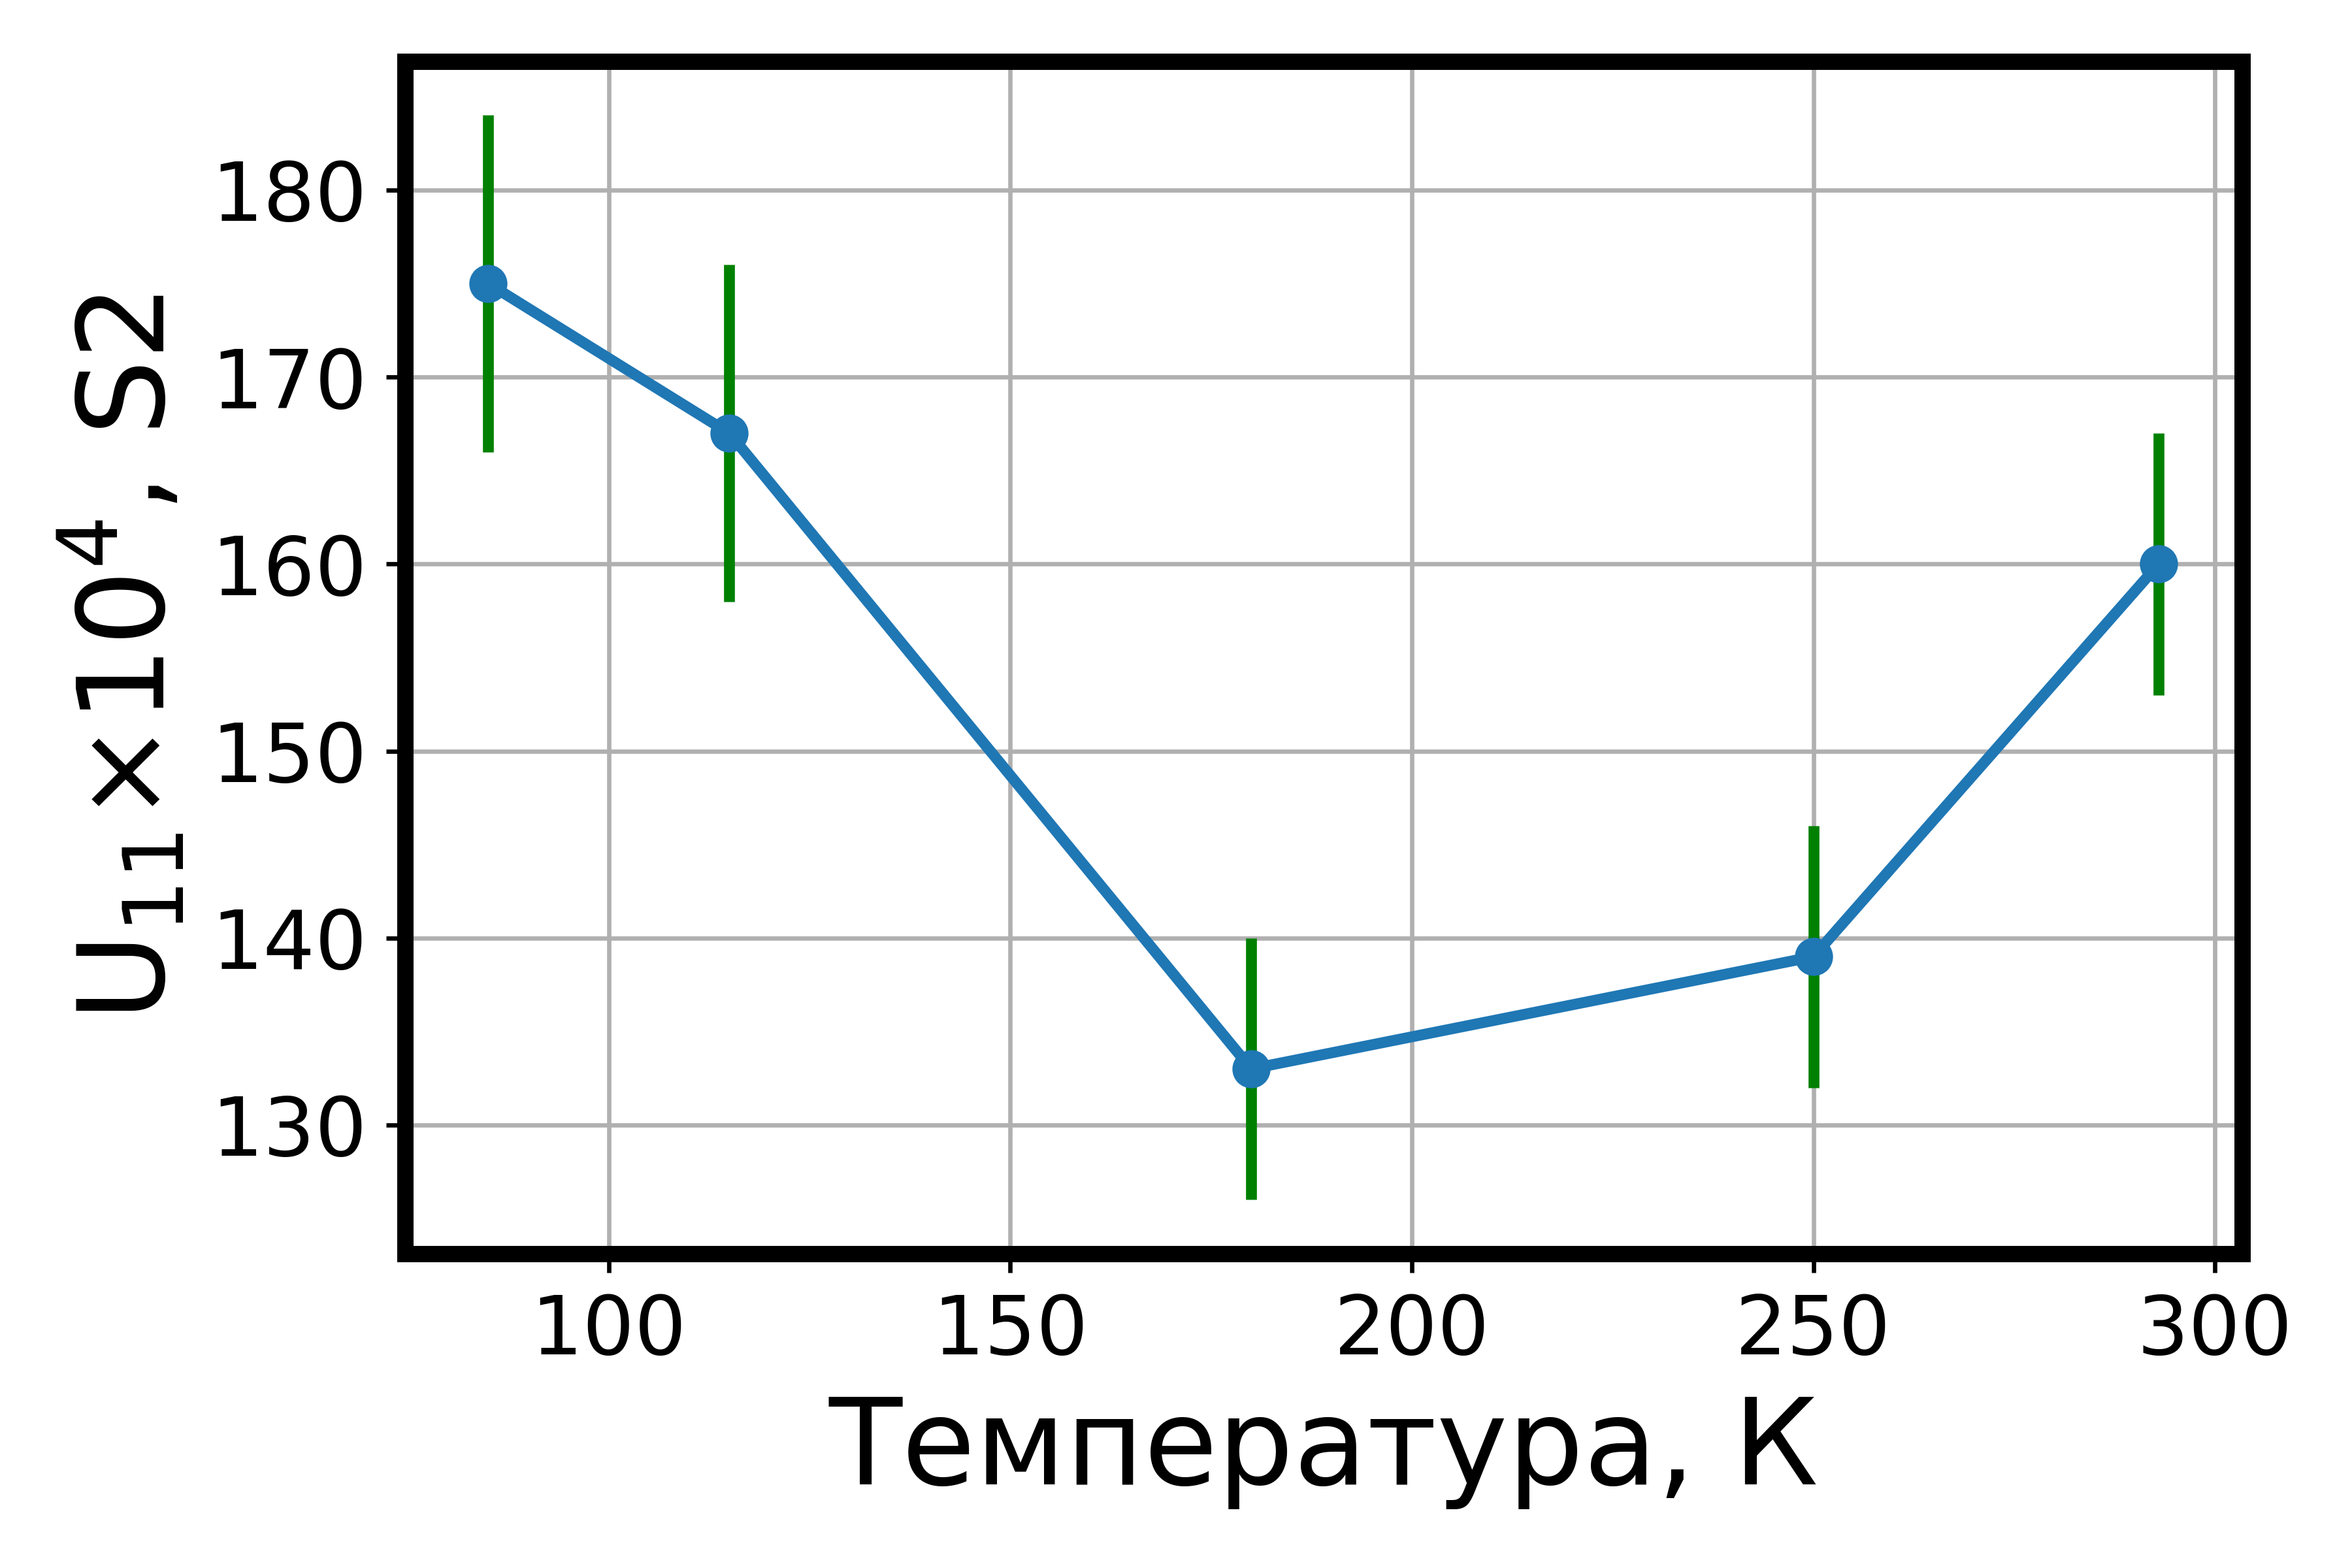
\includegraphics[width=0.9\linewidth]{structure_Ueq} \\ б)
%  \end{minipage}

%      \caption[Значение заселенности позиции атома Cu2 (а) и изменение значения коэффициента атомарного смещения для позиции атома S2 (б) в диапазоне температур от 85 до 293~К синтетического теннантита Cu\textsubscript{12}As\textsubscript{4}S\textsubscript{13}]{Значение заселенности позиции атома Cu2 (а) и изменение значения коэффициента атомарного смещения для позиции атома S2 (б) в диапазоне температур от 85 до 293~К синтетического теннантита Cu\textsubscript{12}As\textsubscript{4}S\textsubscript{13}}
 %   \label{img:xray}
%\end{figure}



Экспериментальная и расчётная зависимости теплоёмкости (Рис.~\ref{img:figure4}) от температуры для синтетического теннантита Сu\textsubscript{12}As\textsubscript{4}S\textsubscript{13} и  синтетического мгриита Cu\textsubscript{3}AsSe\textsubscript{3} удовлетворительно совпадают.
По-видимому, эти моды возникают ввиду ассиметричной связи в As(CuS\textsubscript{3})As, как показывает рентгеноструктурный анализ, в структуре теннантита и, аналогично, в синтетическом мгриите. Такие моды уменьшают решеточную теплопроводность и, как следствие, улучшают термоэлектрические свойства.

Анализ влияния изовалентного замещения на температурные зависимости магнитной восприимчивости (Рис.~\ref{img:figure3}) и на спектры комбинационного рассеяния (Рис.~\ref{img:figure_raman}) показывает, что изменение локального окружения меди приводит к изменению температур магнитных изменений и энергий низкоэнергетических фононных мод. В случае синтетического теннантита Cu\textsubscript{12}As\textsubscript{4}S\textsubscript{13} получено, что АФМ упорядочение энергетически более выгодно, чем другие типы состояний.

В \underline{\textbf{заключении}} приведены основные результаты работы и выводы, которые заключаются в следующем:
%% Согласно ГОСТ Р 7.0.11-2011:
%% 5.3.3 В заключении диссертации излагают итоги выполненного исследования, рекомендации, перспективы дальнейшей разработки темы.
%% 9.2.3 В заключении автореферата диссертации излагают итоги данного исследования, рекомендации и перспективы дальнейшей разработки темы.
\begin{enumerate}
						\item На основе анализа экспериментальных данных, полученных в рентгеноструктурных температурных экспериментах, элекронной микроскопии и на основе результатов квантомеханического моделирования, установлено, что
						лавесовский полиэдр сформирован шестью атомами меди, которые лежат в неэквивалентных позициях Cu2 и Cu21, а на структурную формулу синтетического теннантита Сu\textsubscript{12}As\textsubscript{4}S\textsubscript{13} приходится 12 атомов меди.
						\item Через сравнение данных расчётной  и  экспериментальной теплоёмкостей, полученной сканирующей дифференциальной калориметрией и спектроскопии комбинационного рассеяния света при комнатной температуре, показано влияние ассиметричной связи As(CuS\textsubscript{3})As, возникающей ввиду наличия неэквивалентных позициий Cu2 и Cu21, на размягчение фононных мод в структуре синтетического теннантита Сu\textsubscript{12}As\textsubscript{4}S\textsubscript{13}.
						\item Методами рентгеноструктурного анализа, сканирующей дифференциальной калориметрии, магнитометрии и первопринципных расчётов обнаружен фазовый переход второго рода в синтетическом теннантите Сu\textsubscript{12}As\textsubscript{4}S\textsubscript{13} при температуре 124 К.
						\item Методами сканирующей дифференциальной калориметрии, магнитометрии и спектроскопии комбинационного рассеяния света выявлены  низкоэнергетические фононные моды (ввиду  ассиметричной связи в (As,Sb)(Cu(S, Se)\textsubscript{3})(As,Sb)) в  соединениях из группы тетраэдритов-теннантитов. Найденные значения энергий фононных мод лежат в диапазоне от 5 до 40~мэВ.
						\item На основе результатов работы и опубликованных литературных данных рассмотрено влияние изовалентного замещения в Cu--(As,Sb)--S на значения температур фазовых переходов второго рода.

\end{enumerate}



%\newpage
%При использовании пакета \verb!biblatex! список публикаций автора по теме
%диссертации формируется в разделе <<\publications>>\ файла
%\verb!../common/characteristic.tex!  при помощи команды \verb!\nocite!

\ifthenelse{\equal{\thebibliosel}{0}}{% Встроенная реализация с загрузкой файла через движок bibtex8
  \renewcommand{\refname}{\large \authorbibtitle}
  \nocite{*}
  \insertbiblioauthor                          % Подключаем Bib-базы
  %\insertbiblioother   % !!! bibtex не умеет работать с несколькими библиографиями !!!
}{% Реализация пакетом biblatex через движок biber
  \insertbiblioauthor                          % Подключаем Bib-базы
  \insertbiblioother
}
         % Содержание автореферата


\end{document}